% Leslie Lamport hat LaTeX entwickelt, um dem Anwender das Schreiben
% spezieller Dokumente zu vereinfachen. Um den europäischen/deutschen
% Vorstellungen eines Layouts zu entsprechen, hat Markus Kohm analoge
% Dokumentklassen entwickelt (Koma-Klassen)

% Diese Dokumente sind
% im Original    extern              Koma       extern
% 1. article                         scrartcl
% 2. report                          scrreprt
% 3. book                            scrbook
% 4. letter                          scrlttr2
% 5. slide                                      beamer
% 6.             poster                         tikzposter
% 7.                                            komacv bzw. europecv
% Das Layout ist im Original amerikanischen Vorstellungen ensprechend!

% Der Aufbau ist immer

% Kopf des Dokumentes
% ===================
\documentclass[ngerman,               % in eckigen Klammern stehen
                                      % optionale Angaben, hier: ngerman
                                      % - es werden Trennmuster nach
                                      %   _n_euer deutscher Recht-
                                      %   schreibung geladen
                                      % - wenn das Zusatzpaket babel
                                      %   geladen ist, kann der Autor
                                      %   länderspezifische
                                      %   Befehle, beispielsweise für
                                      %   Anführungszeiche direkt
                                      %   eingeben
                                      % typographische Regeln:
                                      % in der scrreprt-Klasse beginnt
                                      % jedes Kapitel auf einer
                                      % neuen Seite, leere Seiten wie
                                      % die Zusammenfassung
                                      % erhalten keine Seitennummer,
                                      % ebensowenig Titelseiten, es
                                      % werden alle(!!!) Seiten intern
                                      % nummeriert, die Titelseite
                                      % hat die Nummer 1, die
                                      % Seitennummerierung erfolgt
                                      % unten mittig
               a4paper,               % Ausgabe auf DIN A4 Seiten
             % draft,                 % Satzspiegelfehler werden
                                      % angezeigt, Abbildungen werden
                                      % nicht ausgegeben
               fleqn,                 % math. Formeln werden mit festem
                                      % Einzug von links dargestellt
                     ]{scrartcl}       % die Klasse scrbook erfordert
                                      % \frontmatter
                                      %     vor Titel, Vorwort, Bezeichnungen
                                      %     und Inhaltsverzeichnis (m!)
                                      % \mainmatter
                                      %     vor dem eigentlichen Text
                                      % \appendix
                                      %     vor dem Anhang
                                      % \backmatter
                                      %     vor Glossar, Bibliographie (m!)
                                      %     und Index
\usepackage{beamerarticle}            % um das Erstellen von Präsentationen
                                      % zu ermöglichen

% Einstellungen
% =============

% Da die Einstellungen sich von Dokument zu Dokument kaum verändern,
% ist es sinnvoll, diese an einer zentralen Stelle abzulegen und von
% dort zu laden. Dies geschieht völlig transparent mit dem Befehl
% \input{<Pfad>}, dem als Argument eine Datei mit (relativem) Zugriffs-
% pfad übergeben wird
%23456789012345678901234567890123456789012345678901234567890123456789012
\wlog{This is twp-cfg, the common configuration file all documents
  (JHf)}

% Einstellungen werden in LaTeX vor allen Dingen durch das Einbinden
% von Paketen vorgenommen:
% \usepackage[parameter]{package}

\usepackage{iftex}              % Test des Formatierers, durch \if...
                                % können Anpassungen an den Prozessor
                                % vorgenommen werden
\ifluatex                       % wenn mit dem neuen TeX-Prozessor,
                                % der mehr Fontarten unterstützt,
                                % gearbeitet wird:
                                % - pk-Fonts (Pixelfonts, nicht
                                %   skalierbar, alt)
                                % - pfb-Fonts (Fonts, die durch Kurven
                                %   beschrieben werden, skalierbar,
                                %   entwickelt von Adobe->Acrobat
                                %   Reader)
                                % - otf/ttf-Fonts (Fonts, die durch
                                %   Kurven beschrieben werden,
                                %   skalierbar, entwickelt von Apple
                                %   und Microsoft, um Adobe-Lizenzen
                                %   zu sparen)
  %---- Eingabezeichensatz --------------------------------------------
                                % luatex unterstützt utf-8, also keine
                                % Festlegung des Eingabezeichensatzes
                                % erforderlich
  %---- Grundfont -----------------------------------------------------
  \usepackage{fontspec}         % Festlegen der Fontverwaltung für
                                % LuaTeX.
  \defaultfontfeatures{Renderer=Basic, Ligatures=TeX}
  \fontspec{Latin Modern Roman}
  \setmonofont[Scale=0.85]{Luxi Mono Regular} % muss aktiviert werden,
                                % falls das Paket installiert ist
\else
  %---- Eingabezeichensatz --------------------------------------------
  \usepackage[utf8]{inputenc}   % Eingabe deutscher Umlaute
                                % Unix/Linux: utf8
                                % Unix/Linux: latin1 (alt)
                                % Windows: cp1250
  %---- Grundfont -----------------------------------------------------
  \usepackage[T1]{fontenc}      % ec-Fonts
  \usepackage{lmodern}          % wg. der lm-Fonts (keine bitmap-Fonts!)
\fi

%---- Sprachauswahl ---------------------------------------------------
\usepackage{babel}              % um deutsche Bezeichnungen benutzen
                                % zu können, es wird der Parameter aus
                                % dem Kopf des Dokumentes benutzt.

%---- Verwaltung der Bibliographie, muss nach babel geladen werden ----
                                % Verwaltung der
                                % Bibliographie durch
\usepackage[backend=biber,      % Biber und biblatex
            autolang=other,     % Trennung gemäß der mit
                                % babel gesetzten Sprache
            style=alphabetic,   % Verweise ähnlich zu
                                % alpha.bst: XXX00
            citestyle=alphabetic, % mehrere Titel eines
                                % Autors werden XXX00a,
                                % XXX00b, ... zitiert
            giveninits=false,   % Vornamen werden nicht
                                % abgekürzt
            ]{biblatex}
\usepackage[babel,german=quotes]{csquotes} % Titel werden
                                % in deutsche Gänsefüßchen
                                % gesetzt
\addbibresource{../../shared/latex_course.bib}   % muss mit
                                % .bib-Datenbanken gefüllt werden
\ifluatex\else
  \usepackage{babelbib}         % fuer eine dazu passende Bibliographie,
                                % luatex kennt seine eigene
                                % Bibliographieverwaltung
\fi
\defbibheading{bibliography}[Literaturverzeichnis]{\chapter*{#1}}

%---- Sonstiges ------------------------------------------------------
% \PassOptionsToPackage{debugshow,final}{graphicx} % bei Bedarf zu
                                % aktivieren
\usepackage{graphicx}           % Vorbereitung der Graphiken
% \graphicspath{{...}{...}}     % muss mit entsprechenden Pfaden
                                % gefüllt werden, hier
\graphicspath{%                 % weitere Pfade können nach dem
  {../../shared/figures}%       % gleichen Muster hinzugefügt werden
}
\usepackage{listings}           % zur Darstellung von Code aller Art
\lstset{                        % Einstellungen des listings-Paketes
  language=tex,                 % es wird TeX\LaTeX-Code formatiert
  style=colored,                % der Hintergrund und spezielle Befehle
                                % werden farbig dargestellt,
  escapechar=@,                 % mit dem @-Zeichen gibt es die
                                % Möglichkeit,
                                % "ausgezeichneten" Text zu zeigen
}
%\usepackage{isodate}            % wg. \printdate{date}
\usepackage{booktabs}           % wg. \toprule, ...
                                % für typografisch korrekte Linien
\usepackage{moreverb}           % zum Schreiben von Texten in externe
                                % Dateien
\usepackage{tikz}               % TikZ ist kein Zeichenprogramm
\usetikzlibrary{trees}          % Produzieren von Baumstrukturen

\usepackage{pgfplots}           % Darstellung von Funktionen
\pgfplotsset{width=7cm,compat=1.18} % Standardbreite und Kompatibilitätslevel

\usepackage{amsmath}            % für die einfachere Eingabe math. Gleichungen,
                                % muss/sollte als Standard genutzt werden
\usepackage{rotating}           % für die nicht horizontale Textausrichtung
\usepackage{xspace}             % \wg. \xspace: fügt ein Leerzeichen an einen
                                % Text an, außer der Text ist von einem
                                % Punktuationszeichen gefolgt

                                % die nächsten Pakete dienen der Einstellung
                                % von Kopf- und Fußzeile
\usepackage[useregional]{datetime2}  % das Paket zur Darstellung von Tag und
                                % Uhrzeit in einem Format, das im deutschen
                                % Sprachbereich üblich ist
%\renewcommand{\dateseparator}{.}% das übliche Trennzeichen
\newsavebox{\NameAndDate}       % Name und Datum werden nur einmal bestimmt
                                % und dann zum späteren Gebrauch gespeichert
\usepackage[headsepline, footsepline]{scrlayer-scrpage} % das ist das
                                % eigentliche Paket, wir wollen Kopf- und
                                % Fußzeile durch Linien abtrennen

\pagestyle{scrheadings}         % das schaltet das neue Seitenlayout ein
\setkomafont{pagehead}{\normalfont\bfseries} % die Kopfzeile fett
\ifoot{\usebox{\NameAndDate}}   % Name und Datum innen auf der Seite
\AtBeginDocument{%              % wenn \begin{document} erreicht wird,
  \sbox{\NameAndDate}{%
    \footnotesize\textsf{%
      N.~N.: Meine eigene Probearbeit, \today--\DTMcurrenttime%
    }
  }
}

\usepackage{ifthen}             % zur Unterstützung logischer Bedingungen

%---- Bezuege --------------------------------------------------------
% gemäß der cleveref Dokumentation müssen diese Pakete als letzte
% geladen werden
\usepackage{varioref}           % Voraussetzung für cleveref
\usepackage[ngerman]{cleveref}  % deutschsprachige Bezuege, nach babel
                                % zu laden

%---- Einstellungen ---------------------------------------------------
\setcounter{secnumdepth}{7}     % Anzeige der Gliederungsstufen bis
                                % hinunter auf Ebene 7
\setcounter{tocdepth}{7}        % Inhaltsverzeichnis zeigt
                                % Gliederungsstufen bis
                                % hinunter auf Ebene 7, gebraucht wird
                                % das höchstens für technische
                                % Dokumentationen
\newlength{\myWidth}            % universelle Längenangabe, die
                                % jeweils passen gesetzt wird

%---- Eigene Definitionen ---------------------------------------------
\author{Jobst Hoffmann}
\title{Ein erstes \LaTeX-Dokument mit der Dokumentklasse
\texttt{scrartcl}}       % \texttt{<Inhalt>} formatiert <Inhalt>
                         % mit einer dicktengleichen Schriftart

% Hier werden nun eigene Befehle definiert, eine genaue Anleitung
% zur Definition eigener Befehle folgt später:
% \cs:    command sequence, das Argument wird als Befehl formatiert
\NewDocumentCommand{\cs}{m}{\texttt{\char92#1}}
% \farg:  fixed argument, das Argument wird als festes Argument eines
%        Befehls formatiert
\NewDocumentCommand{\farg}{m}
{%
  {\texttt{\{#1\}}}%
}
% \farg:  fixed optional argument, das Argument wird als optionales
%         Argument eines Befehls formatiert
\NewDocumentCommand{\foarg}{m}
{%
  {\texttt{[#1]}}%
}
% \marg:  mandatory argument, das Argument wird als verpflichtendes,
%         aber frei zu wählendes Argument eines Befehls formatiert
\NewDocumentCommand{\marg}{m}
{%
  {\texttt{\{}\(\langle\)\textit{#1}\(\rangle\)\texttt{\}}}%
}
% \meta:  das Argument wird als Beschreibung eines Objektes benutzt
\NewDocumentCommand{\meta}{m}
{%
  {\ensuremath{\langle}\textit{#1}\ensuremath{\rangle}}%
}
% \oarg:  optional argument, das Argument wird als optionales,
%         frei zu wählendes Argument eines Befehls formatiert
\NewDocumentCommand{\oarg}{m}
{%
  {\texttt{[}\(\langle\)\textit{#1}\(\rangle\)\texttt{]}}%
}
% \Cee: der Buchstabe C als Name der Programmiersprache,
%       \xspace sorgt dafür, dass das Kommando bei Bedarf
%       mit einem Leerzeichen ergänzt wird
\NewDocumentCommand{\Cee}{}{\textsc{C}\xspace}

% in dieser Datei werden alle Zusatzpakete mittels
% \usepackage{<package>} geladen

% Trick: verhindere zweifaches Einlesen dieser Datei
\csname SwitchCfgLoaded\endcsname   % Dies ist die Konstruktion des
                                    % Befehls \SwitchCfgLoaded
\let\SwitchCfgLoaded\endinput

\typeout{This is switch-cfg.tex, the single source publishing configuration
file}

% boc: define flags
% flags, die das Formatierungsziel beschreiben
\newboolean{isBook}             % alle flags sind mit
\newboolean{isArticle}          % false initialisiert
\newboolean{isArticleTC}
\newboolean{isReport}
\newboolean{isPresentation}
\newboolean{isPoster}
\newboolean{useBeamerarticle}
% eoc: define flags

% boc: set flags
% mache die folgenden Tests formatierbar
\makeatletter                   % damit ist "@" ein Buchstabe,
                                % ein Befehl darf nun ein "@"
                                % enthalten!
\@ifclassloaded{scrbook}{       % formatiere als Buch
  \setboolean{isBook}{true}
}{                              % formatiere nicht als Buch
  \@ifclassloaded{scrreprt}{    % formatiere als Report
    \setboolean{isReport}{true}
  }{                            % formatiere nicht als Report
    \@ifclassloaded{scrartcl}{  % formatiere als Artikel
      \setboolean{isArticle}{true}
      \@ifclasswith{scrartcl}{twocolumn}{ % zusätzlich:
                                % zweispaltiger Artikel
        \setboolean{isArticleTC}{true}
      }{}                       % einspaltiger Artikel
    }{                          % formatiere nicht als Artikel
      \@ifclassloaded{beamer}{  % formatiere als Präsentation
        \setboolean{isPresentation}{true}
        \@ifpackageloaded{beamerposter}{ % zusätzlich:
                                % formatiere als Poster
          \setboolean{isPoster}{true}
          \defbibheading{bibliography}[]{}
        }{}
      }{}                       % formatiere nicht als
                                % Präsentation
    }
  }
}
\@ifpackageloaded{beamerarticle}{ % zusätzlich:
  % benutze Paket zum Wegdefinieren vom beamer-Befehlen
  \setboolean{useBeamerarticle}{true}
}{}
\makeatother    % @ darf nicht mehr in einem Befehl auftauchen
% eoc: set flags

% hier stehen Einstellungen, die für fast alle Dokumentklassen gebraucht
% werden, Ausnahmen werden weiter unten definiert
\def\sFactor{1.0}               % Variablen werden mittels des
                                % Original-TeX-Kommandos
                                % \def\<cmd-name>{} gesetzt.
                                % \<cmd-name> gilt gruppenweit
                                % und kann durch ein weiteres
                                % \def einfach umgesetzt werden

% boc: use flags
% kombinierte Fälle werden hier abgehandelt, dadurch wird eine
% tiefe Schachtelung vermieden
\ifthenelse{\boolean{isArticleTC} \or \boolean{isPoster}}{
  \usepackage{multicol}             % Um den Text nicht zu breit
                                    % werden zu lassen, wird er
                                    % in einer Umgebung
                                    % "multicols" geschrieben,
                                    % dies erzeugt zwei oder
                                    % mehr Spalten
  \setlength{\columnsep}{1em}       % Platz zwischen den Spalten
  \setlength\columnseprule{0.1em}   % Es wird eine optische
                                    % Trennung durch eine
                                    % senkrechte Linie erzeugt.
}{}
\ifthenelse{\not \boolean{isPresentation}}{
  \ifthenelse{\boolean{useBeamerarticle}}{ % für die Vorlesung ist dieser
    \renewcommand{\frametitle}[1]{} % Befehl unbekannt, in den Projekten
  }{                             % nicht (wg. beamerarticle)
    \newcommand{\frametitle}[1]{}   % Deshalb muss hier mit
  }                              % \newcommand{cmd}[args]{def}
                                 % gearbeitet werden, in den
                                 % Projekten mit
                                 % \renewcommand{cmd}[args]{def}
                                 % Allgemein kann das gelöst werden,
                                 % indem getestet wird, ob ein Paket,
                                 % das nur für die Vorlesung
                                 % gebraucht wird, geladen ist
}{}
% eoc: use flags

% boc: distinguish classes
\ifthenelse{\boolean{isBook}}{
  % dies ist der Standardfall, hier braucht nichts weiter
  % gemacht zu werden
}{
  % kein Buch, deshalb: definiere Kommandos weg, die nicht
  % in einem Buch auftreten können
  %
  % \let \Kommando \neuesKommando macht Folgendes:
  % wenn der TeX-Compiler auf \Kommando trifft, wird statt dessen
  % \neuesKommando ausgeführt
  \let\frontmatter\relax    % \relax ist das "leere" Kommando, das
                            % immer ohne Auswirkungen aufgerufen
                            % werden kann
  \let\mainmatter\relax
  \let\backmatter\relax
  \ifthenelse{\boolean{isReport}}{
  }{
    % kein Buch, kein Report => kein \chapter, also herunterstufen
    % der Gliederungshierarchie, kann fast beliebig fortgesetzt
    % werden...,
    \let\chapter\section
    \let\section\subsection
    \let\subsection\subsubsection

    \ifthenelse{\boolean{isArticle}}{
      % ------- Beginn Spezialfall: 2-spaltiger Artikel ----------
      \ifthenelse{\boolean{isArticleTC}}{
        % hier müssten Faktoren auftreten, die Bilder auf
        % \columnwidth skalieren
      }{}
      % ------- Ende Spezialfall 2-spaltiger Artikel -------------
    }{
      \ifthenelse{\boolean{isPresentation}}{
        \AtBeginSubsection[]{%   Am Anfang einer \subsection wird
                             %   eine eigene Folie generiert
          \begin{frame}<beamer|handout>%
              \begin{block}{}
                  \insertsubsectionhead
              \end{block}
          \end{frame}
        }

        % ------- Beginn Spezialfall Poster ---------------------
        \ifthenelse{\boolean{isPoster}}{

          \def\sFactor{2.83}    % = \sqrt{2}^3,
                                % wg. DIN A4 -> DIN A0/2

          \renewcommand{\maketitle}{% Umdefinieren des bekannten
                                % Kommandos:
                                % \maketitle darf keine eigene Seite
                                % erzeugen!
            \begin{center}%
                \LARGE\inserttitle\\% Zugriff auf die internen Daten
                \normalsize\insertinstitute%
            \end{center}%
          }
          \def\onslide<+->{}    % korrigiere \onslide-Fehler für
                                % Poster
        }{}
        % ------- Ende Spezialfall Poster -----------------------

      }{}
    }
  }
}
% eoc: distinguish classes

\defbeamertemplate*{footline}{ACUAS theme}{%
  \begin{beamercolorbox}[wd=\paperwidth, ht=0.025\paperheight,
      dp=0.005\paperheight]{palette primary}%
      \begin{pgfpicture}
          \pgfusepath{use as bounding box}
          \pgfsetlinewidth{0.8pt}
          \pgftransformshift{\pgfpointanchor{current page}{south west}}
          \pgftransformshift{\pgfpoint{0.03\paperwidth}{0.05\paperheight}}
          \pgfpathmoveto{\pgfpointorigin}
          \pgfpathlineto{\pgfpoint{0.88\paperwidth}{0pt}}
          \pgfusepath{stroke}
          \pgfrememberpicturepositiononpagetrue
      \end{pgfpicture}%
      \usebeamerfont{author}%
      \hspace{0.03\paperwidth}%
      \hbox to 0pt{%
        \copyright{} \jhfb@published{}~%
        \insertshortauthor
        -- \insertshorttitle{} -- \today{}%
      }%
      \hspace{\fill}%
      \insertframenumber
      \hbox to 0.09\paperwidth{}%
  \end{beamercolorbox}%
  \vskip5pt%
}

% in dieser Datei werden Kommandos zum Umschalten zwischen verschiedenen
% Zielformaten (Buch, Report, Artikel, ...)


% merke: ein späterer Titel überschreibt einen früher gesetzten Titel,
% in der scrreprt-Dokumentenklasse erscheint der Titel auf einer
% eigenen Seite
\author{Prof. Dr. Jobst Hoffmann}
\title{Ein erstes \LaTeX-Dokument mit der Dokumentklasse
  \ifthenelse{\boolean{isReport}}{%
    \texttt{scrreprt}%
  }{%
    \texttt{scrartcl}%
  }}
                         % \texttt{<Inhalt>} formatiert <Inhalt>
                         % mit einer dicktengleichen Schriftart
                         % im Vergleich zur ansonsten eingesetzten
                         % Proportionalschrift

% Rumpf des Dokumentes
\begin{document}
\frontmatter                    % es wird mit kleinen, römischen Zahlen
                                % gezählt

% \maketitle                    % die automatisch erzeugte
                                % Titelseite, dies erfordert
                                % die Angabe des Autors und des
                                % Titels in den Einstellungen,
                                % kann für eine Bachelor-, ...
                                % Arbeit nicht benutzt werden!

\makeatletter
\@ifclassloaded{scrartcl}{
  \maketitle{}
}{
% die selbst entworfene Titelseite, die evtl.
% automatisch angepasst werden kann
\begin{titlepage}

% die Leerzeilen bedeuten immer das Ende bzw. den Beginn eines neuen Absatzes,
% ohne eine Leerzeile wird der laufende Text fortgesetzt

% die Ortsangabe soll einheitlich rechtsbündig gesetzt werden, dafür wird
% die Angabe in einen Kasten
% (\parbox[position][height][inner position]{width}{text}) gepackt, der
% passend verschoben wird

% die Box soll rechtsbündig erscheinen, um waagerechten Leerraum zu erhalten,
% benutzt man \hspace{length}. length kann eine variable Größe ein, mit der
% Platz aufgefüllt wird: \fill

% eine geratene Größe für eine Breite ist manchmal ausreichend, meistens
% aber nicht
\settowidth{\myWidth}{\sffamily\large Angewandte Mathematik und Informatik}
%                     ^ die Auswahl und die Größe des Fonts sind wichtig,
%                       sonst stimmen Größen nicht überein
\hspace{\fill}\parbox{\myWidth}{
  % da mehrere Zeilen in einem anderen Font gesetzt werden sollen, benutzt
  % man Befehle, die gruppenintern gelten
  % \scshape        % Kapitälchen (sc: small caps), alle Buchstaben werden
                    % groß geschrieben, die Großbuchstaben ein bisschen
                    % größer, entspricht nicht dem Corporate Design der FH
  \sffamily         % serifenloser Font
  \raggedleft       % rechtsbündiger Satz
  \large
  Fachhochschule Aachen Campus Jülich

  Medizintechnik und Technomathematik

  Angewandte Mathematik und Informatik
}

% eine gute Einteilung von Titelseiten erfolgt nach dem Drittelprinzip
% oder nach dem Golgenen Schnitt
% Drittelprinzip (um 90° gedreht):
%     2/3      1/3
% +----------+-----+
% |          -     |
% +----------+-----+
%
% Goldener Schnitt (um 90° gedreht):
%       a       b
% +----------+-----+
% |          -     |
% +----------+-----+
%    a:b = (a+b):a
%

\vspace{80pt}
\rule{\textwidth}{2pt}

\begin{center}
\Huge \textsf{\bfseries Meine eigene Probearbeit}

% um senkrechten Leerraum zu erhalten, beginnt man den Absatz mit
% einem \vspace{length}. length ist eine Größe, die in einer
% beliebigen Einheit angegeben werden kann, normalerweise in pt
% pt: point, 1 pt ist der 1/72,27 Teil eines inches (1 in = 2,54 cm),
% 10 pt entsprechen ungefähr 3 mm.
\vspace{20pt}
\Large Bachelorarbeit von N.~N.      % ~: bedeutet einen nicht umbrechbaren
                              %     Zwischenraum, das Fehlen dieses
                              %     Zwischenraumes wäre ein schwerer
                              %     typographischer Fehler, ...
                              % N.~N.: aus dem Lateinischen
                              %     - nomen nominandum: ein noch zu
                              %       benennender Name
                              %     - nomen nescio: ich weiß den Namen
                              %       (noch) nicht
\end{center}

  \rule{\textwidth}{2pt}

\vspace{15pt}
\begin{center}
 Jülich, Dezember 2022
\end{center}

\end{titlepage}
}
\makeatother % die selbst entworfene Titelseite

\ifthenelse{\not \boolean{isBook}}{%
  \begin{abstract}              % die abstract-Umgebung gibt es
                                % nicht in der scrbook-Klasse!
      Hier steht eine kurze Zusammenfassung des Inhaltes, es geht hier um
      den Aufbau eines Artikels, insbesondere um die geeignete Gliederung.
  \end{abstract}
}{}

\tableofcontents

% die Gliederung erfolgt in bis zu 7 Ebenen, abhängig von der Klasse
%   Ebene     Klasse                   Befehl (einfachen Form)
%   0.        scrbook/scrreprt         \chapter{<Titel>}
%   1.        alle                     \section{<Titel>}
%   2.        alle                     \subsection{<Titel>}
%   3.        alle                     \subsubsection{<Titel>}
%   4.        alle                     \paragraph{<Titel>}
%   5.        alle                     \subparagraph{<Titel>}
%   6.        alle, nicht im Original  \subsubparagraph{<Titel>}


\mainmatter                     % Umschaltung auf arabische Ziffern

\chapter{Einleitung}   % Einleitung, Hauptteil und Schluss
                       % dürfen niemals in der fertigen Arbeit
                       % stehen, da muss die Autorin bzw. der Autor
                       % sich etwas Passendes einfallen lassen.

Hier steht der Inhalt des Dokumentes, weiteres siehe im n\"achsten
Beispiel. Der erste Absatz wird ohne Einzug formatiert, wenn er
einer \"Uberschrift folgt.

Weitere Absätze bekommen einen Einzug, wie hier deutlich zu sehen ist.
Das soll an dieser Stelle reichen.

In dieser Arbeit wird gezeigt, wie man mit \LaTeX{} arbeitet. Dazu
wird in \cref{chap:TeX} auf die Struktur eines wissenschaftlichen
Dokumentes eingegangen, dabei wird ein spezieller Augenmerk auf die
Befehlsstruktur von \LaTeX{} gerichtet (\cref{sec:befehlsstruktur}).


\chapter{Arbeiten mit \TeX/\LaTeX}% durch dieses %-Zeichen wird
\label{chap:TeX}                  % Leerraum vermeiden, der zu einer
                                  % falschen Nummerierung führen kann
                                  % \label: setzt eine Marke,
                                  % auf die ich mich an andere Stelle
                                  % beziehen kann.

In dieser kleinen Einführung wird beschrieben, wie man mit \LaTeX{} arbeitet.
\LaTeX{} ist ein Makropaket, das von Leslie Lamport auf der Basis
von \TeX{} \cite{knuth_86:tex_book} entwickelt worden ist. Die aktuelle
Entwicklung geschieht durch "`The \LaTeX{} project"', sie ist im Internet
unter zu verfolgen.

% eine Kurzform der Überschrift, die für das Inhaltsverzeichnis
% geeignet ist erzeugt man mit einem optionalen Argument
\section[Die Befehlsstruktur]{Die Befehlsstruktur von \TeX/\LaTeX}%
\label{sec:befehlsstruktur}

% die Nummerierung wird automatisch korekt erzeugt, wenn die
% Gliederung korrekt ist, eine fehlerhafte Gliederung wird durch 0.
% in der Überschrift angezeigt. Für die Hausaufgaben ist eine
% fehlerhafte Nummerierung ein Ausschlusskriterium
\subsection{\TeX: Einfache Befehle -- Primitive} % das doppelte
           % Minuszeichen
           % ist der sogenannte n-dash, es wird immer dann eingesetzt,
           % wenn ein _deutscher_ Gedankenstrich gebraucht wird

Jedes Zeichen ist ein einfacher Befehl: setze das Zeichen in der
aktuellen Schriftart und der aktuellen Größe an die aktuelle
Position, verändere die aktuelle Position um die Breite des Zeichens.
Es gibt aber Zeichen, die eine besondere Bedeutung haben. Wenn man
diese im Text benötigt, muss man eine Ersatzdarstellung benutzen. Im
Regelfall ist es ein vorweggestellter Gegen-/Rückwärtsschrägstrich
(backslash).
\begin{itemize}                 % Listenumgebungen werden später behandelt
  \item Das \%-Zeichen leitet Kommentar ein.
  \item Das \$-Zeichen leitet in \TeX den einfachen Mathematikmodus ein und
    aus.
  \item Das \(\backslash\)-Zeichen leitet Befehle ein, der Befehl endet mit
    dem ersten Nichtbuchstaben. Wird nach einem Befehl ein Leerzeichen
    benötigt, muss man dieses entweder durch einen weiteres
    \(\backslash\)-Zeichen gefolgt von einem Leerzeichen oder durch ein
    Paar von Gruppenklammern erzeugen: Vergleiche \LaTeX und \LaTeX\ und
    \LaTeX{} und auch \LaTeX.
  \item Geschweifte Klammern (\{ und \}) definieren Gruppen. Dinge, die in
    einer Gruppe definiert sind, sind außerhalb der Gruppe unbekannt.
  \item Das Doppelkreuz \# beschreibt Parameter.
  \item Das kaufmännische Und (\&) wird für das Setzen von Tabellen
    gebraucht.
  \item Der Unterstrich (\_) leitet einen Index ein, gilt nur im
    Mathematikmodus.
  \item Das Dach (\^{}) leitet eine Potenz ein, gilt nur im
    Mathematikmodus.
  \item Die Tilde (\~{}) stellt einen Leerraum dar, der nicht umgebrochen
    werden kann.
\end{itemize}

\subsection{\LaTeX: Einfache Befehle}

\LaTeX{} hat die Befehlsstruktur von \TeX{} übernommen, es gibt bei vielen
Befehlen wie bei den Gliederungsbefehlen optionale Parameter, die sich auf
die Ausführung/Darstellung auswirken. Ein einfacher Befehl hat damit die
Syntax
\begin{lstlisting}[style=colored]
@\cs{\meta{Kommandoname}}\oarg{opt. Parameter}\marg{verpflichtende Parameter}@
\end{lstlisting}

Zusätzlich hat \LaTeX{} den Begriff der Umgebung eingeführt: In einer
Umgebung gibt es zusätzliche Kommandos, die außerhalb der Umgebung
unbekannt sind. Auch eine Umgebung kann optionale Parameter benutzen, diese
werden an das einführende Kommando in eckigen Klammern angehängt.
\begin{lstlisting}
\begin{@\meta{Umgebungsame}@}@\oarg{Optionen}@
    ...
\end{@\meta{Umgebungsame}@}
\end{lstlisting}


\subsection{Gliederung/Strukturierung eines Dokumentes}

Ein wissenschaftliche Arbeit zeichnet sich durch ein paar Dinge aus:
\begin{enumerate}
  \item Eine Gliederung entsprechend dem hier vorliegenden Vorbild.

    Diese wird benutzt, um dem Leser den Überblick über den Inhalt und
    das Verständnis des Inhaltes zu erleichtern. Mit einer Gliederung
    kann man den Leser auf wichtige Dinge vorbereiten, man kann auch
    Rückverweise geben.

    Dies geschieht mit den Kommandos
    \lstinline[mathescape]|\label{$\meta{Marke}$}| und
    \lstinline[mathescape]|\cref{$\meta{Marke}$}|. Dabei muss Marke in
    beiden Fällen identisch sein, ein Tippfehler führt zu
    Fehlermeldungen, im Text erscheint \textbf{??}, um den Fehler
    sichtbar zu machen.

\end{enumerate}



\subsection{Weitere Untergliederung Teil 4}

Hier wird gezeigt, wie man auf das Inhaltsverzeichnis und die
Nummerierung der Unterabschnitte Einfluss nehmen kann. Standarmäßig
wird nummeriert bis zur \lstinline|\subsection|, wenn weitergehend
nummeriert werden soll, muss man entsprechende Grenzen setzen
\begin{lstlisting}
  \setcounter{secnumdepth}@\marg{Tiefe}@
\end{lstlisting}
\meta{Tiefe} gibt die Stufe an, bis zu der nummeriert werden soll.

\subsubsection{Unterunterabschnitt 1}

Kein wichtiger Inhalt

\subsubsection{Unterunterabschnitt 2}

Kein wichtiger Inhalt

\paragraph{Unterunterunterabschnitt 1}

Noch weniger wichtig

\paragraph{Unterunterunterabschnitt 2}

Noch weniger wichtig

\subparagraph{Unterunterunterunterabschnitt 1}

Noch viel weniger wichtig


\subparagraph{Unterunterunterunterabschnitt 2}

Noch viel weniger wichtig, wie zuvor

% \subsubparagraph{Unterunterunterunterunterabschnitt 1}

Noch viel, viel weniger wichtig


\section[Zweiter Unterabschnitt]{Zweiter Unterabschnitt zu dem Hauptteil,
  der in der Zukunft einen wesentlich aussagekräfigeren Titel bekommen
  muss}

\section[Listen]{Weitere Gliederung eines Dokumentes mit Listen}

Hier folgen Beispiele, die beim Selbststudium ausprobiert werden.

\section[Tabellen]{Übersichtliche Darstellung von Informationen mittels
  Tabellen}

\subsection{Die \texttt{tabular}-Umgebung}

Die Spaltenorientierung wird festegelgt durch: c -- centered (zentriert), l
-- left aligned (linksbündig), r -- right aligned (rechtsbündig), die
Zellen einer Tabelle innerhalb einer Zeile werden beendet durch \& oder
\cs{}\cs{}. Eine Tabelle, die durch die \texttt{tabular}-Umgebung erzeugt
wird, wird als ein(!!!!) Zeichen behandelt. Eine Tabelle wird an der
aktuellen Zeile mit optionalen Angaben ([c] oder [t] oder [b])
ausgerichtet. Die Ausrichtung erfolgt an der oberen/unteren Linie, wenn sie
vorhanden ist, ansonsten an der Grundlinie der ersten bzw. letzten
Tabellenzeile.

1.%
\begin{tabular}{|c|l|r|}
  \hline
  a & bcd & e \\
  \hline
  fgh & l & mno \\
  \hline
  pq & rs & uv \\
  \hline
\end{tabular}%
2.%
\begin{tabular}[t]{|c|l|r|}
  \hline
  a & bcd & e \\
  \hline
  fgh & l & mno \\
  \hline
  pq & rs & uv \\
  \hline
\end{tabular}%
3.%
\begin{tabular}[b]{|c|l|r|}
  \hline
  a & bcd & e \\
  \hline
  fgh & l & mno \\
  \hline
  pq & rs & uv \\
  \hline
\end{tabular}%
Schluss

1.%
\begin{tabular}{|c|l|r|}
  \hline
  a & bcd & e \\
  \hline
  fgh & l & mno \\
  \hline
  pq & rs & uv \\
  \hline
\end{tabular}%
2.%
\begin{tabular}[t]{|c|l|r|}
    % \hline
  a & bcd & e \\
  \hline
  fgh & l & mno \\
  \hline
  pq & rs & uv \\
  \hline
\end{tabular}%
3.%
\begin{tabular}[b]{|c|l|r|}
  \hline
  a & bcd & e \\
  \hline
  fgh & l & mno \\
  \hline
  pq & rs & uv \\
  % \hline
\end{tabular}%
Schluss

Die hier gezeigten Linien dienen allein der Verdeutlichung der Ausrichtung,
in einem Text zur Veröffentlichung haben Linien außer den unten gezeigten
nichts zu suchen, sie werden als typographische Fehler betrachtet und
verhindern die Anerkennung des Moduls! Linien zur Erzeugung von Grafiken
haben ihre Bedeutung.

Wie eine Tabelle als ein Zeichen betrachet wird, so wird auch eine Zelle
als ein Zeichen betrachtet, insbesondere die mit dem oben erwähnten
Spaltenbeschreibungen. Daraus ergibt sich, dass ein Text in einer Zelle
nicht umgebrochen werden kann:

\begin{tabular}{|c|l|r|}
  \hline
  a & bcd: dies sind der zweite bis vierte Buchstabe des Alphabets & e \\
  \hline
  fgh & l & mno \\
  \hline
  pq & rs & uv: dies sind der einundzwanzigste und zweiundzwanzigste
            Buchstabe des Alphabets \\
  \hline
\end{tabular}%

Die so entstandene Tabelle läuft aus dem Satzspiegel heraus. Auch dies ist
ein typographischer Fehler, der die Anerkennung des Moduls verhindert!

Lösung des Problems: \texttt{p\{\meta{Breite}\}}

\begin{tabular}{|c|p{4cm}|p{5cm}|}
  \hline
  a & bcd: dies sind der zweite bis vierte Buchstabe des Alphabets & e \\
  \hline
  fgh & l & mno \\
  \hline
  pq & rs & uv: dies sind der einundzwanzigste und zweiundzwanzigste
            Buchstabe des Alphabets \\
  \hline
\end{tabular}%

Wie Breiten gewählt werden, die zum Ausfüllen des Satzspiegels führen, wird
später gezeigt.

\texttt{p\{\meta{Breite}\}} führt zur linksbündigen Ausrichtung der Spalte.
Wenn bei "`kurzen"' Zellen die Ausrichtung erhalten bleiben soll, greift
man zur Definition einer Zelle mit
\lstinline|\multicolumn{cols}{pos}{text}|:

\begin{tabular}{|c|p{4cm}|p{5cm}|}
  \hline
  a & bcd: dies sind der zweite bis vierte Buchstabe des Alphabets &
                                                                     \multicolumn{1}{r|}{e} \\
  \hline
  fgh & l & \multicolumn{1}{r|}{mno} \\
  \hline
  pq & rs & uv: dies sind der einundzwanzigste und zweiundzwanzigste
            Buchstabe des Alphabets \\
  \hline
\end{tabular}%

\subsection{Grafiken mit der \texttt{tabular}-Umgebung}

Die Darstellung von Beziehungen erfolgt häufig mit Rechtecken:

% +--------+        +-------------------------+
% |        |        |                         |
% |  TeX   |        |    Prozessor            |
% | Code   |        |                         |
% +--------+        +-------------------------+

\begin{tabular}{p{1cm}|p{2cm}|p{1cm}|p{4cm}|}
  \cline{2-2}\cline{4-4}
  & \TeX-Code & \(\rightarrow\)& Prozessor \\
  \cline{2-2}\cline{4-4}
\end{tabular}

Auch baumartige Zusammenhänge lassen sich so zeigen:

% +-----------------------+
% |                       |   besteht aus 2 Zellen!
% |     Wurzel            |   => \multicolumn
% |                       |
% +-----------+-----------+
% |
% +-------------+-------------+
% |                           |
% +---+----+        +-------------+-----------+
% |        |        |                         | Diese Zellen
% | linker |        |  rechter Knoten         | werden in
% | Knoten |        |                         |
% +--------+        +-------------------------+

Der Ansatz ist damit

\begin{tabular}{*{7}{p{1cm}}}  % *: Spaltenbeschreibung wird wiederholt
  \cline{4-5}         % 7: 7-mal
  &  & & \multicolumn{2}{|c|}{Wurzel} &  \\
  \cline{4-5}
  &  & & \multicolumn{1}{c|}{} & \\
\end{tabular}

\subsection{Die \texttt{table}-Umgebung}

Die \texttt{table}-Umgebung ist eine gleitende Umgebung, d.\,h. sie
erscheint nicht unbedingt dort, wo sie im Quelltext steht, sondern bei
Bedarf etwas davor oder sogar ganz weit hinten im Text.

Tabellen können sehr lang sein und somit nicht auf den "`Rest"' der Seite
passen:

\begin{tabular}{c}
  a\\
  b\\
  c\\
  d\\
  e\\
  f\\
  g\\
  h\\
  i\\
  j\\
  k\\
  l\\
  m\\
  n\\
  o\\
  p\\
  q\\
  r\\
  s\\
  t\\
  u\\
  v\\
  w\\
  x\\
  y\\
  z
\end{tabular}

Eine solch lange Tabelle wird deshalb in eine \texttt{table}-Umgebung
eingefügt, vgl. dazu \cref{tab:alphabet}.

\begin{table}[bt]   % gibt zulässige Postionen an, muss nicht
                    % eingehalten werden
                    % b: am Ende einer Seite
                    % t: am Anfang einer Seite
                    % h: nach Möglichkeit hier
                    % p: auf einer eigenen Seite
    \centering      % die Tabelle wird seitenzentriert formatiert
    \caption{Das Alphabet mit 26 Kleinbuchstaben} % Tabellen haben
                    % Überschriften, weil sie nach unten wachsen können,
                    % anders wäre es ein typografischer Fehler, ...
    \label{tab:alphabet}
    \begin{tabular}{c}
      \toprule     % dicke Linie
      \textbf{Kleinbuchstabe}\\
      \midrule     % dünnere Linie
      a\\
      b\\
      c\\
      d\\
      e\\
      f\\
      g\\
      h\\
      i\\
      j\\
      k\\
      l\\
      m\\
      n\\
      o\\
      p\\
      q\\
      r\\
      s\\
      t\\
      u\\
      v\\
      w\\
      x\\
      y\\
      z\\
      \bottomrule % dicke Linie zum Abschluss, muss nach \\
      % stehen
    \end{tabular}
\end{table}


\section{multi file-Dokumente}

\subsection[Zerlegen und Einbinden von Textteilen]{Zerlegen eines Textes in
  Teile und Einbinden der Teile mit \cs{input}\farg{file}}

Um Übersicht zu behalten, lagert man gemeinsam genutzte Inhalte in
eigene, externe Dateien aus. Beispiele dazu sind die bekannten
Konfigurationsdateien \texttt{tw-cfg.tex} usw.

Diese Dateien werden mit dem Kommando
\begin{lstlisting}
\input@\marg{Dateiname}@
\end{lstlisting}
in das aktuelle Dokument eingebunden. \meta{Dateiname} bezieht sich
auf eine Datei im Suchpfad, wenn keine Pfadangabe im Dateinamen
enthalten ist. Der Suchpfad kann ausgegeben werden mittels
\begin{lstlisting}
kpsewhich -expand-var='$TEXINPUTS'
\end{lstlisting}
Die Ausgabe startet immer mit einem Punkt, der das aktuelle Verzeichnis
bezeichnet. Wenn \meta{Dateiname} keinen Punkt enthält, wird die
Dateinamenserweiterung \texttt{.tex} angenommen.

Ein einfaches Beispiel arbeitet mit drei Dateien \texttt{a.tex},
\texttt{b.tex} und \texttt{c.tex}:

a

b

c


Vergleiche dazu

a
%
b
%
c


Das Kommentarzeichen hinter dem \cs{input}-Befehl sorgt dafür, dass
das Zeilenende ignoriert wird, diese drei Zeilen entsprechen also

a
b
c


Keine Leerzeichen erhält man mit

a%
b%
c


wenn also den einzelnen Zeichen direkt ein Kommentarzeichen folgt.

Dem Dateinamen darf eine Pfadangabe vorausgestellt werden, diese
kann einen relativen Pfad (\texttt{../}) oder einen absoluten Pfad
(\texttt{/}) bedeuten, eine Laufwerksangabe (Windows) ist möglich.

Ein Befehl, der noch wichtig sein könnte (große Dokumente) ist der
\lstinline|include|-Befehl, vgl. dazu das Skript.

\subsection{Einbinden spezieller Inhalte}

Unter speziellen Inhalten werden hier Dinge verstanden, die
\begin{enumerate}
  \item nicht als Text vorliegen wie Bilder (.jpg, .png),
  \item die anderweitig als (Quell-)Text bereitgestellt werden
    (Programm-Code, Bibliographie-Datenbanken),
  \item die zwar aus \TeX-Code bestehen, aber der Einfachheit halber
    nicht im Dokument selbst aufgeführt werden sollen (Fehlersuche,
    Wiederverwertbarkeigt).
\end{enumerate}
Für alle diese Fälle gibt es Pakete, die den Autor optimal unterstützen.

\subsubsection{Einbinden von Bildern}

Es müssen zwei Arten von Bildern unterschieden werden:
\begin{enumerate}
  \item Rastergraphiken, wie sie von Kameras aufgenommen werden -- diese
    können nur in begrenztem Maße skaliert werden (nicht über die
    Originalgröße hinaus) und
  \item Vektorgraphiken, die mit entsprechenden Werkzeugen erzeugt wurden
    -- diese können beliebig skaliert werden.
\end{enumerate}

\paragraph{Das Einbinden von Rastergraphiken}

Als Basis für die nächsten Beispiele wird ein Bildschirmfoto mit einer
Größe von 3840x2160 Pixel genommen.

Das Einbinden von Rastergraphiken erfolgt mit dem
\lstinline|\includegraphics|-Befehl, der von den Paketen \texttt{graphics}
-- die einfache Variante, bietet nur wenige Optionen -- und
\texttt{graphicx} -- die umfangreichere Variante, bietet eine Vielzahl von
Möglichkeiten der Einflussnahme auf das einzubindende Bild --
bereitgestellt wird.

Alle externen Pakete werden mit dem \lstinline|\usepackage|-Befehl und
eventuellen Optionen bereitgestellt.

% \textwidth: Breite des Satzspiegels,
% verwandt dazu:
% \paperwidth: Breite der Seite
% \linewidth: Breite der aktuellen Zeile
\includegraphics[width=0.7\textwidth]{bildschirmfoto} % das Bild auf
                                % die 0,7-fache Breite der Seite skaliert

Ohne Skalierung sind Fotos häufig zu groß, wie auf der nächsten Seite zu
sehen ist. Um Bilder/Fotos wie Tabellen sinnvoll zeigen zu können, müssen
Sie in eine entsprechende gleitende Umgebung gepackt werden,
vgl. \cref{fig:bildschirm} auf Seite \pageref{fig:bildschirm}. Wenn man
Pech hat, erscheint das Bild am Ende des gesamten Textes.
\begin{figure}[htb]
    \centering%                   Eine Abbildung sollte immer zentriert sein
                                % \centering sorgt dafür, das der Inhalt
                                % einer Umgebung zentriert wird, damit korrekt
                                % zentriert wird, muss der Befehl mit "%"
                                % abgeschlossen werden, ansonsten steht die
                                % Abbildung ein Leerzeichen zu weit nach rechts!
                                % Ein fehlendes "%"-Zeichen ist ein
                                % typographischer Fehler, ...
    \includegraphics{bildschirmfoto}
    \caption{Ein Bildschirmfoto} % Bilder haben Unterschriften!
    \label{fig:bildschirm}
\end{figure}

\subparagraph{Optionen des includegraphics-Befehls}

\begin{enumerate}
  \item \texttt{width}: s.\,o.
  \item \texttt{scale}: skaliert ein Foto um den gegebenen Faktor,
    vgl. \cref{fig:bildschirm_05}.
    \begin{figure}[htb]
        \centering%
        \includegraphics[scale=0.05]{bildschirmfoto}
        \caption{Ein Bildschirmfoto auf 5\% skaliert} % Bilder haben
        % Unterschriften!
        \label{fig:bildschirm_05}
    \end{figure}

  \item \texttt{bounding box, bb}: schneidet im Zusammenhang mit der Option
    \texttt{clip} einen Bereich zur Darstellung aus dem Bild aus,
    vgl. \cref{fig:bildschirm_bb}. Statt der Kombination \texttt{bb} und
    \texttt{clip} kann die Option \texttt{trim} benutzt werden.

    Der abzuschneidende Bereich wird durch ein Quadrupel von vier Maßen
    bezeichnet, die das Abschneiden von links, unten, rechts und von oben
    angeben.  Bei Rastergrafiken sollte sinnvollerweise die Einheit
    \texttt{px} für Pixel angegeben werden, ansonsten eine der üblichen
    \TeX-Einheiten.
    %                             (urx, ury)
    % +---------------------------+
    % |                           |
    % |                      +    |
    % |              +            |
    % |                           |
    % +---------------------------+
    % (llx, lly)
    \begin{figure}[htb]
        \centering%
        % Maß des Fotos: 3840x2160px, es bleiben übrig
        %                     rechte Hälfte
        %                            obere Hälfte des verbleibenden Restes
        %                                   linke Hälfte des verbleibenden
        %                                   Restes, also drittes Viertel
        %                                   von links
        %                                         zweites Viertel von oben
        \includegraphics[trim=1920px 1080px 810px 540px, clip,
          width=\textwidth]{bildschirmfoto}
        \caption{Ein Bildschirmfoto an den Rändern abgeschnitten} % Bilder haben
                                % Unterschriften!
        \label{fig:bildschirm_bb}
    \end{figure}
\end{enumerate}


\paragraph{Das Einbinden von Vektorgraphiken}

.pdf-Dateien sind Vektorgrafiken\footnote{Vektorgrafiken werden
  beispielsweise mit \texttt{inkscape} erzeugt}, können also mit dem
\lstinline|\includegraphics{imagefile}|-Befehl in den Text eingebaut
werden, vgl. \cref{fig:raster}.
\begin{figure}[htb]
    \centering%                   muss mit einem % beendet werden
    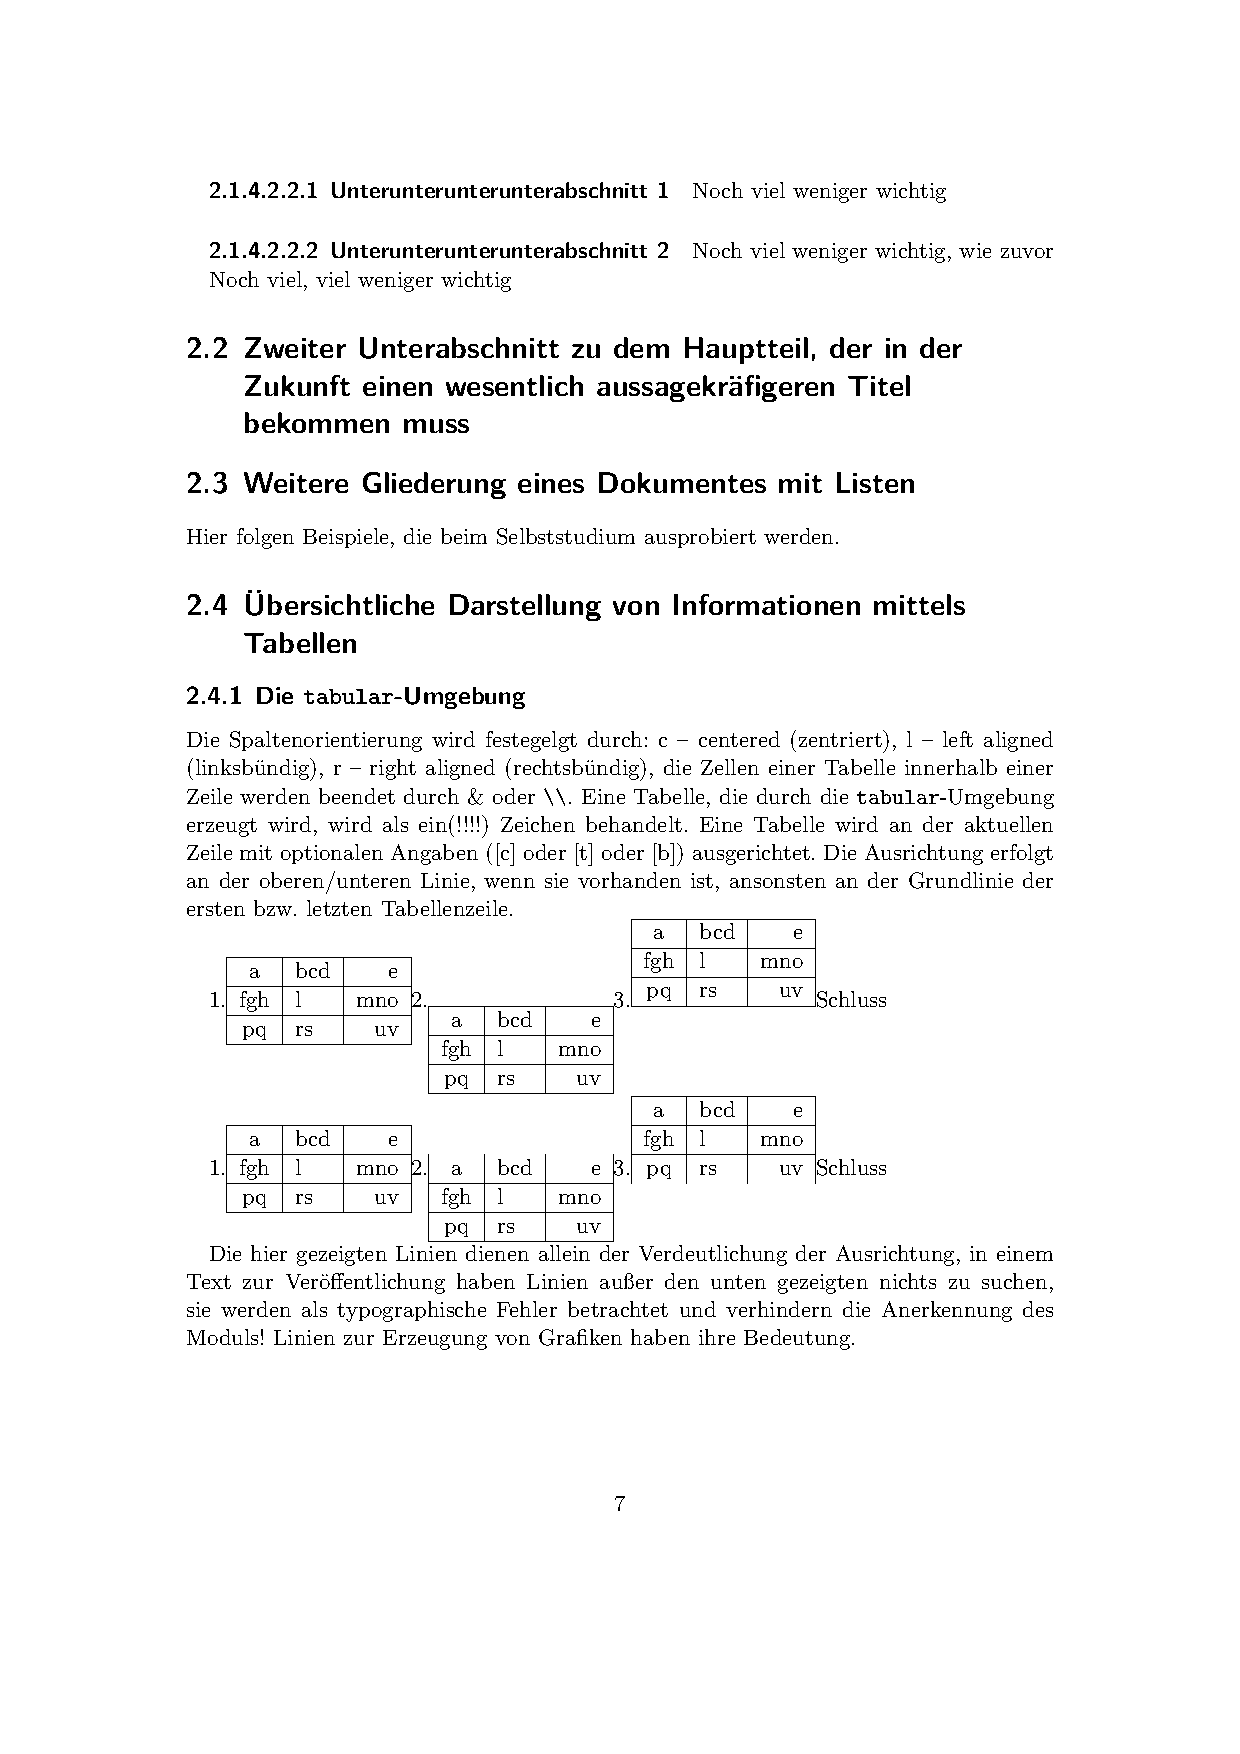
\includegraphics[width=0.7\textwidth]{latex_course_07.pdf} % Erweiterung
                                % muss angegeben werden
    \caption{Ein Ausschnitt aus der vorliegenden Arbeit} % Bilder haben
                                % Unterschriften!
    \label{fig:raster}
\end{figure}


\section{Grafiken und \LaTeX}
\label{sec:grafiken-und-latex}

Es gibt etliche Pakete, mit denen (Linien-)Grafiken mit \LaTeX-Befehlen erzeugt
werden können:
\begin{enumerate}
  \item \texttt{pict2e} als Erweiterung der \LaTeX-immanenten
    \texttt{picture}-Umgebung,
  \item \texttt{pstricks}, das entsprechend der Dokumentation
    \textit{PostScript macros for Generic \TeX} bereitstellt, und
  \item \texttt{tikz}, was für \textit{TikZ is kein Zeichenprogramm} steht,
    und eine große Sammlung von Bibliotheken bereitstellt, die auf PGF
    basieren. Die Originaldokumentation sagt dzu aus: "`\textit{PGF is a
      TeX macro package for generating graphics. It is platform- and
      format-independent and works together with the most important TeX
      backend drivers, including pdftex and dvips. It comes with a
      user-friendly syntax layer called TikZ.}"'
  \item \ldots{}
\end{enumerate}
Beispiele zu den erstgenannten Paketen finden sich in, hier werden nur
\texttt{tikz} und ein paar Erweiterungen vorgestellt.

\subsection{\texttt{tikz} als universelles Makropaket zum Programmieren von
  Grafiken}
\label{sec:als-univ-makr}

\texttt{tikz} stellt zwei Möglichkeiten der Erzeugung von Grafiken bereit:
\begin{enumerate}
  \item Den Befehl \cs{tikz}, der \texttt{tikz}-Makros als Argument(e)
    benötigt, und der \textit{inline}-Grafiken wie
    \tikz \draw (0, 0) -- (1mm, 1mm); erzeugt, eine fehlende Einheit wird
    als cm interpretiert.
  \item Die Umgebung \texttt{tikzpicture}, die eigenständige Grafiken aus
    \texttt{tikz}-Makros erzeugt.
\end{enumerate}
\textbf{Hinweis:} Jedes Makro muss mit einem Semikolon abgeschlossen werden.


\subsubsection{Elementare Beispiele}
\label{sec:elementare-beispiele}

Um die Beispiele besser verstehen zu können, wird zu einem Trick gegriffen:
\begin{enumerate}
  \item mit der Umgebung \texttt{verbatimwrite} aus dem Paket \texttt{moreverb}
    werden Kommandos in eine Datei geschrieben.
  \item mit dem Kommando \lstinline|\lstinputlisting| wird diese Datei
    eingelesen und wörtlich wiedergegeben.
  \item mit dem Kommando \lstinline|\input| wird diese Datei
    eingelesen und formatiert.
\end{enumerate}

\begin{enumerate}
  \item Ein Linienzug wird erzeugt mit
\begin{verbatimwrite}{../../shared/figures/linienzug.tex}
\tikz \draw[thick,rounded corners=2pt] % eine "dicke" Linie, Ecken werden
                                       % abgerundet
(0,0) -- (0,2) -- (1,3.25) -- (2,2) -- % -- verbindet zwei Punkte durch
(2,0) -- (0,2) -- (2,2) -- (0,0) -- (2,0);  % eine Gerade
\end{verbatimwrite}
    \lstinputlisting{../../shared/figures/linienzug.tex}

    \tikz \draw[thick,rounded corners=2pt] % eine "dicke" Linie, Ecken werden
                                       % abgerundet
(0,0) -- (0,2) -- (1,3.25) -- (2,2) -- % -- verbindet zwei Punkte durch
(2,0) -- (0,2) -- (2,2) -- (0,0) -- (2,0);  % eine Gerade

  \item Ein Linienzug mit Ecken wird erzeugt mit
\begin{verbatimwrite}{../../shared/figures/linienzug_eck.tex}
  \tikz \draw[thick]                   % eine "dicke" Linie
  (0,0) -| (2,2) |- (4, 4);            % Punkte werden über Eck
                                       % verbunden
\end{verbatimwrite}
    \lstinputlisting{../../shared/figures/linienzug_eck.tex}

      \tikz \draw[thick]                   % eine "dicke" Linie
  (0,0) -| (2,2) |- (4, 4);            % Punkte werden über Eck
                                       % verbunden

  \item Eine Kurve wird erzeugt mit
\begin{verbatimwrite}{../../shared/figures/kurve.tex}
\begin{tikzpicture}
    \filldraw [gray] (0,0) circle [radius=2pt]
    (1,1) circle [radius=2pt]
    (2,2) circle [radius=2pt]
    (2,0) circle [radius=2pt];
    \draw (0,0) .. controls (1,1) and (2,2) .. (2,0);
\end{tikzpicture}
\end{verbatimwrite}
    \lstinputlisting{../../shared/figures/kurve.tex}

    \begin{tikzpicture}
    \filldraw [gray] (0,0) circle [radius=2pt]
    (1,1) circle [radius=2pt]
    (2,2) circle [radius=2pt]
    (2,0) circle [radius=2pt];
    \draw (0,0) .. controls (1,1) and (2,2) .. (2,0);
\end{tikzpicture}

  \item (Wiederholte) Kreise in einem verschiedenfarbig gezeichneten Gitter anordnen:
\begin{verbatimwrite}{../../shared/figures/kreise_wdh.tex}
\tikz {%
  % Gitter zur besseren Einordnung der Kreise
  \draw[step=.5cm, blue] (-0.6,-0.6) grid (9.6,0.6);
  \draw[step=.5cm, help lines, red, xshift=0.25cm, ystep=0cm] (-0.6,-0.6) grid (9.3,0.6);
  \draw[step=.5cm, help lines, green, yshift=0.25cm, xstep=0cm] (-0.6,-0.6) grid (9.6,0.3);

  \foreach \x in {0,...,9}
    \draw (\x,0) circle (0.4cm);       % Mittelpunkt und Radius eines Kreises
}
\end{verbatimwrite}
    \lstinputlisting{../../shared/figures/kreise_wdh.tex}

    \tikz {%
  % Gitter zur besseren Einordnung der Kreise
  \draw[step=.5cm, blue] (-0.6,-0.6) grid (9.6,0.6);
  \draw[step=.5cm, help lines, red, xshift=0.25cm, ystep=0cm] (-0.6,-0.6) grid (9.3,0.6);
  \draw[step=.5cm, help lines, green, yshift=0.25cm, xstep=0cm] (-0.6,-0.6) grid (9.6,0.3);

  \foreach \x in {0,...,9}
    \draw (\x,0) circle (0.4cm);       % Mittelpunkt und Radius eines Kreises
}

  \item Koordinaten an Punkten notieren:
\begin{verbatimwrite}{../../shared/figures/punkte.tex}
\begin{tikzpicture}
    \draw (0,0) circle [radius=2pt] node [anchor=east]{(0, 0)};
    \draw (1,1) circle [radius=2pt] node [anchor=north]{(1, 1)};
    \fill (2,2) circle [radius=2pt] node [anchor=south]{(2, 2)};
    \draw[thick] (3,1) circle [radius=2pt] node [anchor=north west]{(3, 1)};
    \draw[red, fill=green] (4,0) circle [radius=2pt]
        node [anchor=west, black]{(4, 0)};
\end{tikzpicture}
\end{verbatimwrite}
    \lstinputlisting{../../shared/figures/punkte.tex}

    \begin{tikzpicture}
    \draw (0,0) circle [radius=2pt] node [anchor=east]{(0, 0)};
    \draw (1,1) circle [radius=2pt] node [anchor=north]{(1, 1)};
    \fill (2,2) circle [radius=2pt] node [anchor=south]{(2, 2)};
    \draw[thick] (3,1) circle [radius=2pt] node [anchor=north west]{(3, 1)};
    \draw[red, fill=green] (4,0) circle [radius=2pt]
        node [anchor=west, black]{(4, 0)};
\end{tikzpicture}

  \item Grafische Elemente an bestimmten Stellen positionieren:
\begin{verbatimwrite}{../../shared/figures/node_pos.tex}
\begin{tikzpicture}
    \begin{scope}[name prefix = top-]
        \node (A) at (0,1) {A};
        \node (B) at (1,1) {B};
        \draw (A) -- (B);
    \end{scope}
    \begin{scope}[name prefix = bottom-]
        \node (A) at (0,0) {A};
        \node (B) at (1,0) {B};
        \draw (A) -- (B);
    \end{scope}

    \draw [red] (top-A) -- (bottom-B);
\end{tikzpicture}
\end{verbatimwrite}
    \lstinputlisting{../../shared/figures/node_pos.tex}

    \begin{tikzpicture}
    \begin{scope}[name prefix = top-]
        \node (A) at (0,1) {A};
        \node (B) at (1,1) {B};
        \draw (A) -- (B);
    \end{scope}
    \begin{scope}[name prefix = bottom-]
        \node (A) at (0,0) {A};
        \node (B) at (1,0) {B};
        \draw (A) -- (B);
    \end{scope}

    \draw [red] (top-A) -- (bottom-B);
\end{tikzpicture}


  \item Bäume mit der Bibliothek \texttt{trees} (in \texttt {twp-cfg.tex}
    muss die Zeile
\begin{lstlisting}
\usetikzlibrary{trees}          % Produzieren von Baumstrukturen
\end{lstlisting}
    stehen) konstruieren:
\begin{verbatimwrite}{../../shared/figures/path_tree.tex}
% Voreinstellungen für Elemente des Baumes
\tikzset{directory/.style={rectangle, rounded corners, draw,
        font=\ttfamily, fill=blue!20}}
\tikzset{file/.style={rectangle, draw, font=\ttfamily, fill=green!10}}

\begin{tikzpicture}[level distance=7.5mm]%
    \node[directory] {\ldots} %
        [edge from parent fork down]%
    child[sibling distance=30mm] {node[directory] {a}} %
    child {node[directory] {b-directory} %
      child {node[directory] {c} %
        child{node[file] {MyClass.java}}} %
    }
    child[sibling distance=30mm] {node[file] {README.md}};
\end{tikzpicture}
\end{verbatimwrite}
    \lstinputlisting{../../shared/figures/path_tree.tex}

    % Voreinstellungen für Elemente des Baumes
\tikzset{directory/.style={rectangle, rounded corners, draw,
        font=\ttfamily, fill=blue!20}}
\tikzset{file/.style={rectangle, draw, font=\ttfamily, fill=green!10}}

\begin{tikzpicture}[level distance=7.5mm]%
    \node[directory] {\ldots} %
        [edge from parent fork down]%
    child[sibling distance=30mm] {node[directory] {a}} %
    child {node[directory] {b-directory} %
      child {node[directory] {c} %
        child{node[file] {MyClass.java}}} %
    }
    child[sibling distance=30mm] {node[file] {README.md}};
\end{tikzpicture}

\end{enumerate}


\subsubsection{Das Bezeichnen vorgegebener Abbildungen}
\label{sec:das-beze-vorg}

Es gibt häufig den Fall, dass ein gegebenes Bild mit zusätzlichen
Bezeichnungen versehen werden muss.

Zunächst werden die in einem ungleichmäßig skalierten Bildschirmfoto die
Linien eingezeichnet, die beim \texttt{trim} eingesetzt wurden.

\begin{tikzpicture}
    \tikzset{every ellipse node/.style={draw,
        color=red, text=black, line width=2pt}}
    \pgftext[bottom, left, x=0pt, y=0pt]{% Ausrichtung des Bildes
                                % erfolgt an seiner linken Unterkante,
                                % es wird nicht in x- oder y-Richtung
                                % verschoben
      \includegraphics[width=15cm, height=10cm]{bildschirmfoto}}; % das Bild auf
                                % eine feste Breite skaliert
    \draw[help lines, white, thick] (0, 0) grid (15,10);%
    \draw[red, very thick] (7.5, 0) -- (7.5, 10)
                           (7.5, 5) -- (15, 5)
                           (11.25, 5) -- (11.25, 10)
                           (7.5, 7.5) -- (11.25, 7.5);%
    \node[white] at (9.375, 6.25){trimmed};%
\end{tikzpicture}

Dann wird in einem gleichmäßig skalierten Bildschirmfoto der Kopf des
Nachrichtensprechers markiert.

\begin{tikzpicture}
    \tikzset{every ellipse node/.style={draw,
        color=red, text=black, line width=2pt}}
    \pgftext[bottom, left, x=0pt, y=0pt]{%
      \includegraphics[width=16cm]{bildschirmfoto}}; % das Bild auf
                                % eine feste Breite skaliert
      % \draw[help lines, white, thick] (0, 0) grid (16, 9);%
      \draw[white, very thick] (11.75, 7) ellipse [x radius=0.75cm, y radius=1.5cm];
\end{tikzpicture}


\subsection{\texttt{pgfplots} als Paket zur Darstellung von Funktionen}

Eine häufig auftretende Aufgabenstellung ist die Darstellung beliebiger
Funktionen. Prinzipiell kann das mit den nun bekannten Mitteln von
\texttt{tikz} erledigt werden, besser geeignet ist das Paket \texttt{pgfplots}.
Zusätzlich zum Laden des Paketes sollte in \texttt{twp-cfg.tex} die
Kompatibilitätsstufe vermerkt werden.

\begin{enumerate}
  \item Eine Funktion \(f: \mathcal R \rightarrow \mathcal R\):
\begin{verbatimwrite}{../../shared/figures/r_to_r_gnuplt.tex}
\begin{tikzpicture}
    \begin{axis}            % das Koordinatensystem wird mit
                            % der Umgebung axis erzeugt
        \addplot[           % ein Plot wird hinzugefügt
          id=parable,
          domain=-5:5,      % der Definitionsbereich
        ] gnuplot {4*x**2 - 5}% die Funktion, setzt das Programm
        % gnuplot voraus
        node [pin=180:{$4x^2-5$}]{}; % Legende der Grafik
    \end{axis}
\end{tikzpicture}
\end{verbatimwrite}
    \lstinputlisting{../../shared/figures/r_to_r_gnuplt.tex}

    \begin{tikzpicture}
    \begin{axis}            % das Koordinatensystem wird mit
                            % der Umgebung axis erzeugt
        \addplot[           % ein Plot wird hinzugefügt
          id=parable,
          domain=-5:5,      % der Definitionsbereich
        ] gnuplot {4*x**2 - 5}% die Funktion, setzt das Programm
        % gnuplot voraus
        node [pin=180:{$4x^2-5$}]{}; % Legende der Grafik
    \end{axis}
\end{tikzpicture}


  \item Dieselbe Funktion \(f: \mathcal R \rightarrow \mathcal R\) mit
    \TeX{} als Datenprozessor, zu beachten ist die andere Darstellung der
    Potenz -- gnuplot: \lstinline|4*x**2 - 5|, also zwei Sternchen, \TeX:
    \lstinline|4*x^2-5|.
\begin{verbatimwrite}{../../shared/figures/r_to_r_tex.tex}
  \begin{tikzpicture}
      \begin{axis}            % das Koordinatensystem wird mit
                              % der Umgebung axis erzeugt
          \addplot[             % ein Plot wird hinzugefügt
            domain=-5:5         % der Definitionsbereich
          ] { 4*x^2-5 }         % die Funktion
          node [pin=180:{$4x^2-5$}]{}; % Legende der Grafik
      \end{axis}
  \end{tikzpicture}
\end{verbatimwrite}
    \lstinputlisting{../../shared/figures/r_to_r_tex.tex}

      \begin{tikzpicture}
      \begin{axis}            % das Koordinatensystem wird mit
                              % der Umgebung axis erzeugt
          \addplot[             % ein Plot wird hinzugefügt
            domain=-5:5         % der Definitionsbereich
          ] { 4*x^2-5 }         % die Funktion
          node [pin=180:{$4x^2-5$}]{}; % Legende der Grafik
      \end{axis}
  \end{tikzpicture}


  \item Noch einmal dieselbe Funktion
    \(f: \mathcal R \rightarrow \mathcal R\) mit \TeX{} als Datenprozessor,
    jetzt mit einer zusätzlichen Achsenbeschriftung und einem Vergleich mit
    Messpunkten.
\begin{verbatimwrite}{../../shared/figures/r_to_r_vgl.tex}
  \begin{tikzpicture}
      \begin{axis}[           % das Koordinatensystem wird mit
                              % der Umgebung axis erzeugt,
                              % hier zusätzliche Optionen
            xlabel=\(x\),
            ylabel={\(y=f(x)=4x^2 - 5\)} % {...} wegen der
                              % Leerzeichen
          ]
          \addplot[           % ein Plot wird hinzugefügt
            domain=-5:5,      % der Definitionsbereich
            color=blue,
            mark=x            % berechnete Punkte werden mit
                              % einem x markiert
          ] { 4*x^2-5 }       % die Funktion
          node [pin=180:{$4x^2-5$}]{}; % Legende der Grafik
          \addplot[
            domain=-5:5,
            color=green,
            mark=*
          ]
          coordinates {
            (-4, 59)
            (0, -5)
            (1, -1)
            (2, 9)
            (5, 95)
          };
      \end{axis}
  \end{tikzpicture}
\end{verbatimwrite}
    \lstinputlisting{../../shared/figures/r_to_r_vgl.tex}

      \begin{tikzpicture}
      \begin{axis}[           % das Koordinatensystem wird mit
                              % der Umgebung axis erzeugt,
                              % hier zusätzliche Optionen
            xlabel=\(x\),
            ylabel={\(y=f(x)=4x^2 - 5\)} % {...} wegen der
                              % Leerzeichen
          ]
          \addplot[           % ein Plot wird hinzugefügt
            domain=-5:5,      % der Definitionsbereich
            color=blue,
            mark=x            % berechnete Punkte werden mit
                              % einem x markiert
          ] { 4*x^2-5 }       % die Funktion
          node [pin=180:{$4x^2-5$}]{}; % Legende der Grafik
          \addplot[
            domain=-5:5,
            color=green,
            mark=*
          ]
          coordinates {
            (-4, 59)
            (0, -5)
            (1, -1)
            (2, 9)
            (5, 95)
          };
      \end{axis}
  \end{tikzpicture}

\end{enumerate}


\section{Mathematischer Formelsatz}

Zwei Varianten: \TeX-spezifisch und \LaTeX-spezifisch, letztere ist unbedingt
vorzuziehen!

\begin{tabular}{llll}
  \toprule
  & \TeX & \LaTeX{} lang & \LaTeX{} kurz\\
  \midrule
  \textit{inline} & \lstinline|$ ... $| & \lstinline|\begin{math} ... \end{math}| & \lstinline|\( ... \)| \\
  \textit{display} & \lstinline|$$ ... $$| & \lstinline|\begin{displaymath} ... \end{displaymath}|& \lstinline|\[ ... \]| \\
  \bottomrule
\end{tabular}

\textit{inline} bedeutet: \(3+4=7\), dahingegen wird \textit{display} so
formatiert: \[3+4=7\]. Es gibt viele Automatiken in \TeX: Zahlen werden
automatisch als \textit{inline math} erkannt, es wird automatisch
unterschieden zwischen Bindestrich und Minuszeichen, ebenso wird Vorzeichen
von Operator unterschieden:
\[\mbox{3-4, aber } 3-4=-1\]

Der Mathematikmodus stellt viele zusätzliche Befehle bereit, so wird der
Unterstrich benutzt, um Indizes zu kennzeichnen: \(a_{ij}\).\footnote{Die
  Klammern sind wichtig: \(a_{ij} \ne a_ij\).} Entsprechend wird das Dach
für Exponenten benutzt: \(x^{2}\). Text wird im mathematischen Formelsatz
kursiv gesetzt, Funktionen hingegen aufrecht: \(f(x) = \sin x\). Es gibt
die üblichen mathematischen Funktionen in der Schreibweise
\cs{}\meta{Funktionsname}, also etwa \(\cos \pi = -1\).


\subsection{Skalare Größen/Gleichungen}

Wichtige mathematische Bezeichnungen sind
\(\sum_{i=1}^{n}i=\frac{n\cdot(n+1)}{2}\) oder auch
\[\sum_{i=1}^{n}i=\frac{n\cdot(n+1)}{2}\]

Der \textit{displaymath}-Modus sorgt für größere Zeichen und bessere
Übersicht!

\[\int\limits_{-1}^{1} x dx = 0\]

Für Wurzeln gibt es \lstinline|\sqrt[root]{arg}|: \(\sqrt[3]{27}=3\)

Es ist eine typographische Unart, die Menge der reellen Zahlen mit
\(\mathbb{R}\) zu beschreiben, richtig ist \(\mathcal{R}\).

Grenzwerte werden so geschrieben:
\( \lim\limits_{x\rightarrow0}\frac{\sin x}{x}=0 \mbox{ oder }
\lim_{x\rightarrow0}\frac{\sin x}{x}=0 \) aber
\[
    \lim\limits_{x\rightarrow0}\frac{\sin x}{x}=0 \mbox{ oder }
    \lim_{x\rightarrow0}\frac{\sin x}{x}=0
\]

Im Mathematikmodus gibt es keinen Umbruch!!! Wenn mehrere Zeilen gebraucht
werden, muss man mit geeigneten Umgebungen wie \texttt{eqnarray} arbeiten:
\begin{eqnarray}
  \label{eq:sin}%
  \sin x & = & \sum_{i=0}^{\infty}(-1)^{i}\frac{x^{2i+1}}{(2i+1)!}
  \\
  \label{eq:sin_expl}       & = & x - \frac{1}{3!}x^{3} + \frac{1}{5!}x^{5} - \ldots + \ldots
\end{eqnarray}
\textbf{Hinweise:}
\begin{enumerate}
  \item \texttt{eqnarray} ist eine spezielle Tabelle, es besteht aus drei
    Spalten, das Gleichheitszeichen muss zwischen zwei kaufmännische Unds
    gesetzt werden.
  \item Jede Zeile bekommt automatisch eine Nummer, auf die man sich
    beziehen kann, etwa so: Die Taylorentwicklung der \(\sin\)-Funktion
    wird in Gleichung \ref{eq:sin} gezeigt, Gleichung \ref{eq:sin_expl}
    zeigt die ausgeführte Summenbildung.

    \lstinline|\cref| funktioniert gemäß ...  mit der
    \texttt{eqnarray}-Umgebung nicht, es liefert hier \cref{eq:sin}(?)! Es
    wird empfohlen, die analogen Umgebungen des \texttt{amsmath}-Paketes zu
    benutzen.
  \item \texttt{eqnarray*} liefert keine Nummern.
  \item Eine Nummer kann zeilenweise unterdrückt werden mit dem
    Befehl \lstinline|\nonumber|.
\end{enumerate}

Eine einfachere Beschreibung von mathematischen Zusammenhängen ist mit dem
Paket \texttt{amsmath} möglich, dann funktioniert
auch \lstinline|\cref|. Das obige Beispiel lässt sich dann so schreiben:
\begin{equation}
    \begin{split}
      \label{eq:sin_ams}%
      \sin x &=  \sum_{i=0}^{\infty}(-1)^{i}\frac{x^{2i+1}}{(2i+1)!}
      \\
             &=  x - \frac{1}{3!}x^{3} + \frac{1}{5!}x^{5} - \ldots + \ldots
    \end{split}
\end{equation}
\cref{eq:sin_ams} zeigt die Taylorentwicklung der \(\sin\)-Funktion.

Analog zu \texttt{eqnarray} gibt es  \texttt{align}
\begin{align}
  \label{eq:ams_sin}%
  \sin x &=  \sum_{i=0}^{\infty}(-1)^{i}\frac{x^{2i+1}}{(2i+1)!}
  \\
  \label{eq:ams_sin_expl}        &=  x - \frac{1}{3!}x^{3} + \frac{1}{5!}x^{5} - \ldots + \ldots
\end{align}
Zur Darstellung von Fallunterscheidungen gibt es \texttt{cases}:
\begin{equation}
    \label{eq:fakultaet_00}
    n! =
    \begin{cases}
      1 & n=1\\
      n(n-1)! & n > 1
    \end{cases}
\end{equation}
\cref{eq:fakultaet_00} kommt ohne Text aus, besser ist es mit einer Erklärung,
wie es in \cref{eq:fakultaet_01} gezeigt wird:
\begin{equation}
    \label{eq:fakultaet_01}
    n! =
    \begin{cases}
      1 & \text{für } n=1\\          % lokale Umschltung in den
      n(n-1)! & \text{für den Fall } n > 1    % Textmodus
    \end{cases}
\end{equation}


\subsection{Vektorielle Größen/Gleichungen}

Ein Vektor im \(n\)-dimensionalen Raum wird beschrieben durch
\(\vec{x} \in \mathcal{R}^{n}\). Komponentenweise wird er beschrieben durch
\(\vec{x} = \left(              % \left leitet eine bel. Klammer
    % in der passenden Größe eine
    \begin{array}{c}
      x_{1} \\ \vdots \\ x_{n}  % es gibt neben \vdots (vertical)
      % auch \ldots (lower)
      % \cdots (central)
      % \ddots (diagonal)
      % als Befehle zum Beschreiben einer
      % Folge von Punkten
    \end{array}
\right)                   % \right ist verpflichtend nach einem $\left$
\)

Damit lässt sich ein Gleichungssystem schreiben als
\[
    \underbrace{
      \left(
          \begin{array}{*{4}{c}}
            a_{11} & a_{12} & \cdots & a_{1n} \\
            a_{21} & a_{22} & \cdots & a_{2n} \\
            \vdots & \vdots & \ddots & \vdots \\
            a_{m1} & a_{m2} & \cdots & a_{mn} \\
          \end{array}
      \right)
      \cdot
      \left(
          \begin{array}{c}
            x_{1} \\
            x_{2} \\
            \vdots \\
            x_{n}
          \end{array}
      \right)
    }_{\text{linke Seite}}
    =
    \underbrace{
      \left(
          \begin{array}{c}
            b_{1} \\
            b_{2} \\
            \vdots \\
            b_{n}
          \end{array}
      \right)
    }_{\text{rechte Seite}}
\]
kurz:
\[
    A\cdot\vec{x}=\vec{b}
\]
oder mit Nummerierung der Formel
\begin{equation}
    A\cdot\vec{x}=\vec{b}
\end{equation}


\section{Feinheiten des Drucksatzes mit \TeX/\LaTeX}

\subsection{Gestaltung einer Titelseite}

Bessere Gestaltung einer Titelseite erfolgt durch
\begin{itemize}
  \item besondere Schrifttypen (Fonts) in unterschiedlichen Größen,
  \item grafische Elemente (Linien in unterschiedlichene Dicken und
    Richtungen) und
  \item evtl. Logos.
\end{itemize}

Es wird unterschieden zwischen Brotschrift, wie sie für den laufenden Text
gebraucht wird, und Auszeichungsschrift, die für Überschriften eingesetzt
wird.

Als Brotschrift wird der besseren Lesbarkeit halber eine Serifen-behaftete
Schrift ausgewählt (Standard in \texttt{scr}-Paketen: eine von der Times
abgeleitete Schrift -- auch als Antiqua bezeichnet, da mit einer solchen
Schrift römische Tempel beschrieben worden sind, daher auch der Name
\textit{modern roman} -- , definiert durch die Serifen eine Grundlinie, die
die Augen der Schrift besser folgen lässt).

Als Auszeichungsschrift wird eine Schrift ausgewählt, die viele
Eigenschaften mit der Brotschrift gemeinsam hat, die sich aber dennoch
deutlich unterscheidet (Standard in \texttt{scr}-Paketen: eine serifenlose,
fette Schrift -- als Helvetica bezeichnet).

Diese Schriften werden unterschiedlichen Größen eingesetzt: von {\tiny ganz
  winzig} bis zu {\Huge riesig groß}. \lstinline|\tiny|
und \lstinline|\Huge| sind Schrift\emph{attribute}, die ab sofort bis zum
Gruppenende gelten.

\textnormal{Das ist Brotschrift} und \textsf{das ist Auszeichungsschrift},
\textnormal{das ist normale Brotschrift} und \textsf{\bfseries das ist
  fette Auszeichungsschrift}.

Merkregel: Innerhalb eines laufenden Textes wird \emph{niemals}%
\footnote{typographischer Fehler, \ldots} fett gedruckt, wenn etwas
\emph{hervorgehoben} werden soll, dann durch Betonung
(\textit{emphasize}, \lstinline|\emph|).

Linien können gezeichnet werden
\begin{itemize}
  \item horizontal: \rule{220pt}{2pt}
  \item vertikal: \rule{1pt}{22pt}
\end{itemize}
Die Größenangaben werden typischerweise in pt gemacht. Die Einzelheiten dazu
finden sich im Kommertar zu \texttt{titel.tex}.


\subsection{Nicht-horizontale Textausrichtung}

Der Standard im Drucksatz ist die horizontale Textausrichtung des Fließtextes.
Es gibt aber Situationen, in denen eine andere Ausrichtung sinnvoll oder sogar
erforderlich ist. Dafür gibt es das Paket \texttt{rotating.sty}.

\subsubsection{Gedrehte Tabellen}

Sehr breite Tabellen passen nicht in den Satzspiegel, vgl.
\cref{tab:marokko-brasilien}.
\begin{table}[htb]
    \centering%
    \caption{Statistik des Spiels Marokko - Brasilien}
    \label{tab:marokko-brasilien}
    \begin{tabular}{*{6}{p{2.5cm}}}
      \toprule%
      eigene Tore & gegnerische Tore & gelbe Karten & rote Karten &
                                                                    Abseitstellungen & Ballbesitz \\\midrule
      1 & 0 & 2 & 0 & 5 & 30 \% \\\bottomrule
    \end{tabular}
\end{table}

Die Abhilfe ist die gedrehte Tabelle, vgl.
\cref{tab:marokko-brasilien-sideways}.
\begin{sidewaystable}[p]
    \centering%
    \caption{Statistik des Spiels Marokko - Brasilien}
    \label{tab:marokko-brasilien-sideways}
    \begin{tabular}{*{6}{p{2.5cm}}}
      \toprule%
      eigene Tore & gegnerische Tore & gelbe Karten & rote Karten &
                                                                    Abseitstellungen & Ballbesitz \\\midrule
      1 & 0 & 2 & 0 & 5 & 30 \% \\\bottomrule
    \end{tabular}
\end{sidewaystable}

Die Breite einer Tabelle hängt häufig von den Spaltenüberschriften ab,
wie in den Beispeilen \cref{tab:marokko-brasilien} und
\cref{tab:marokko-brasilien-sideways} gut zu sehen ist.

Eine Spaltenüberschrift kann schmaler werden, wenn sie gedreht wird,
vgl. \cref{tab:marokko-brasilien-narrow}.
\begin{table}[htb]
    \centering%
    \caption{Statistik des Spiels Marokko - Brasilien}
    \label{tab:marokko-brasilien-narrow}
    \begin{tabular}{*{6}{l}}
      \toprule%
      \begin{sideways}    % dreht den Inhalt um 90° gegen den Uhrzeigersinn
          eigene Tore
      \end{sideways} & \begin{rotate}{60} % dreht den Inhalt um 60° gegen
          % den Uhrzeigersinn, fordert keinen eigenen Platz
          % ein, \toprule wird falsch gesetzt
          % ein \settoheight{\gnat}{text} würde hier
          % helfen (vgl. \settowidth{\gnat}{text})
          gegnerische Tore
      \end{rotate} & \begin{turn}{30} % dreht den Inhalt um 30° gegen
          % den Uhrzeigersinn, fordert eigenen Platz
          % ein, \toprule wird richtig gesetzt
          gelbe Karten
      \end{turn} & rote Karten &
                                 Abseitstellungen & Ballbesitz \\\midrule
      1 & 0 & 2 & 0 & 5 & 30 \% \\\bottomrule
    \end{tabular}
\end{table}


\section{Verschiedenes}

Hier werden die Themen behandelt, die
\begin{itemize}
  \item nützlich (eigene Definitionen zur Abkürzung häufig benutzter
    Begriffe, ein Seitenlayout mit Zeitangabe) oder
  \item unverzichtbar (Erstellen einer Bibliographie/eines
    Literaturverzeichnisses)
\end{itemize}
für das Erstellen einer Abschlussarbeit sind.

\subsection{Eigene Definitionen}%
\label{sec:eigene-definitionen}

In \TeX{} ist es möglich, mit dem Makro \lstinline|\def| eigene Makros
zu definieren. Diese werden expandiert, d.\,h. durch ihren Inhalt
ersetzt, bis nur noch Primitive auftreten, die dann in Text umgesetzt
werden. Ein einfaches Beispiel:
\begin{verbatimwrite}{../../shared/texts/def_00.tex}
  \def\dreiA{AAA}
\end{verbatimwrite}
Mit
\lstinputlisting{../../shared/texts/def_00.tex}
wird ein Makro definiert, das seinen Inhalt direkt ausgibt:
  \def\dreiA{AAA}
\dreiA.

\dreiA\hspace{\fill}\dreiA\hspace{\fill}\dreiA

Die Programmierung von \TeX{} ist damit relativ kompliziert und nur
den \TeX nicians zuzumuten.

\subsection{Programmieren mit \LaTeX}

Die Programmierung mit \LaTeX{} ist wesentlich einfacher gestaltet, es gibt
aber für \LaTeXe{} und \LaTeX3 unterschiedliche Schnittstellen. Da \LaTeX3 jetzt
schon überall unter der Haube arbeitet, wird nur diese Schnittstelle
vorgestellt.

\subsubsection{Eigene Funktionen}

Mit \LaTeX3 ist der Begriff Makro und Makroexpansion aus der Sprachbeschreibung
herausgefallen. Es wird zwar in der Syntaxbeschreibung noch von Expandierung
gesprochen, es geht nun aber immer um Funktionen, Variablen und Strukturen.

An dieser Stelle wird nicht in die Interna eingestiegen, sondern es wird
nur die neue Syntax vorgestellt.


\paragraph{Parameterlose Funktionen}

Zur Definition eigener Kommandos gibt es die Funktion
\begin{lstlisting}[escapechar=@]
\NewDocumentCommand@\marg{cmd}\marg{xargs}\marg{def}@
\end{lstlisting}
\meta{cmd} ist der Name der zu definierenden Funktion, der \cs{} muss
aufgeführt werden, \meta{xargs}
beschreibt die Parameter, \meta{def} ist die Definition der Funktion.

Das Beispiel aus \cref{sec:eigene-definitionen} sieht dann so aus:
\begin{verbatimwrite}{../../shared/texts/def_01.tex}
\NewDocumentCommand{\iiiA}        % Funktionen dürfen nicht doppelt
                                  % auftreten
                   {}             % es gibt keine Parameter
                   {AAA}          % es sollen drei As gesetzt werden
\end{verbatimwrite}
\lstinputlisting{../../shared/texts/def_01.tex}

Der Einsatz ist wie oben: \NewDocumentCommand{\iiiA}        % Funktionen dürfen nicht doppelt
                                  % auftreten
                   {}             % es gibt keine Parameter
                   {AAA}          % es sollen drei As gesetzt werden
\iiiA.

Nun etwas sinnvolleres, die Definition einer Abkürzung:
\begin{verbatimwrite}{../../shared/texts/def_02.tex}
\NewDocumentCommand{\JHf}       % Funktionen dürfen nicht doppelt
                                % auftreten
                   {}           % es gibt keine Parameter
                   {Jobst Hoffmann}  % es soll der Name gesetzt
                                % werden
\end{verbatimwrite}
\lstinputlisting{../../shared/texts/def_02.tex}

\NewDocumentCommand{\JHf}       % Funktionen dürfen nicht doppelt
                                % auftreten
                   {}           % es gibt keine Parameter
                   {Jobst Hoffmann}  % es soll der Name gesetzt
                                % werden

Zunächst muss die Definition wieder eingelesen werden, bevor sie
benutzt werden kann: \JHf schrieb diesen Text. Es ist zu beachten,
dass auch eigene Funktionen sich nach der grundsätzlichen Syntax von
\TeX/\LaTeX{} arbeiten: ein Funktionsaufruf endet mit dem ersten
Nicht-Buchstaben. Um also nach dem Namen ein Leerzeichen zu erhalten,
muss der Funktionsaufruf mit \{\} beendet werden: \JHf{} schrieb
diesen Text.

\paragraph{Funktionen mit Parametern}

\meta{xargs} beschreibt die Parameter, die der Funktion übergeben werden
können. Es wird hier nur der Fall beschrieben, dass als Argument ein
einzelnes Token oder mehrere mit geschweiften Klammern \{\} umgebene Token
auftreten. Weitere Parameterarten sind \cite{latex_project_22:xparse} zu
entnehmen.

\meta{xargs} ist eine Folge von Buchstaben, wir benutzen nur \texttt{m} und
\texttt{o}, für jeden dieser Buchstaben mit im Ersatztext der Reihe nach
\lstinline|#1|, \lstinline|#2|, $\ldots$, \lstinline|#9| auftreten, es gibt
auf diese Weise maximal 9 Parameter.


\subparagraph[Umgang mit obligatorischen Parametern]{%
  Umgang mit obligatorischen (engl.: \textit{\_m\_andatory}) Parametern}

Um einen Vektor komponentenweise aufzuschreiben, muss man die
Dimension des zugehörigen Raumes angeben:
\begin{verbatimwrite}{../../shared/texts/def_03.tex}
  \NewDocumentCommand{\vektor}   % Funktionen dürfen nicht doppelt
                                 % auftreten
                     {m}         % es gibt einen verpflichtenden
                                 % Parameter, die Dimension
                     {           % es sollen die Komponenten
                        \ensuremath{(x_{1},  % eines Vektor
                          \ldots, % beschrieben werden
                                 % \ensuremath: unabhängig
                                 % von Mathematik-Modus
                          x_{#1})}
                     }

\end{verbatimwrite}
\lstinputlisting{../../shared/texts/def_03.tex}

  \NewDocumentCommand{\vektor}   % Funktionen dürfen nicht doppelt
                                 % auftreten
                     {m}         % es gibt einen verpflichtenden
                                 % Parameter, die Dimension
                     {           % es sollen die Komponenten
                        \ensuremath{(x_{1},  % eines Vektor
                          \ldots, % beschrieben werden
                                 % \ensuremath: unabhängig
                                 % von Mathematik-Modus
                          x_{#1})}
                     }



\vektor{3}, \vektor{n}

\subparagraph[Umgang mit optionalen Parametern]{%
  Umgang mit optionalen (engl.: \textit{\_o\_ptional}) Parametern}

Was muss getan werden, wenn weitere Vektoren auftreten? Kann mit der Dimension
besser umgegangen werden? Also: standardmäßig wird im \(\mathcal R^{3}\)
gearbeitet, es kann aber auch eine andere Dimension genannt werden.

\begin{verbatimwrite}{../../shared/texts/def_04.tex}
  \NewDocumentCommand{\vektorN}  % Funktionen dürfen nicht doppelt
                                 % auftreten
                     {o m}       % es gibt einen optionalen, den
                                 % Namen, und einen verpflichtenden
                                 % Parameter, die Dimension
                     {           % es sollen die Komponenten
                       \IfNoValueTF{#1}{\def\dimI{3}}{\def\dimI{#1}}
                       \ensuremath{(#2_{1},  % eines Vektor
                       \ldots,   % beschrieben werden
                                 % \ensuremath: unabhängig
                                 % von Mathematik-Modus
                       #2_{\dimI})
                     }
  }

\end{verbatimwrite}
\lstinputlisting{../../shared/texts/def_04.tex}

  \NewDocumentCommand{\vektorN}  % Funktionen dürfen nicht doppelt
                                 % auftreten
                     {o m}       % es gibt einen optionalen, den
                                 % Namen, und einen verpflichtenden
                                 % Parameter, die Dimension
                     {           % es sollen die Komponenten
                       \IfNoValueTF{#1}{\def\dimI{3}}{\def\dimI{#1}}
                       \ensuremath{(#2_{1},  % eines Vektor
                       \ldots,   % beschrieben werden
                                 % \ensuremath: unabhängig
                                 % von Mathematik-Modus
                       #2_{\dimI})
                     }
  }



\vektorN{x}, \vektorN{y}, \vektorN[n]{x}, \vektorN[n]{y}


\subparagraph{Umdefinieren von Umgebungen}

Wenn eine Umgebung nicht so arbeitet, wie der Autor es sich vorstellt,
kann sie umdefiniert werden.

Ein Vers von Wilhelm Busch:
\begin{verse}
  Eins, zwei, drei, im Sauseschritt \\
  eilt die Zeit, wir eilen mit.
\end{verse}

Der Autor wünscht sich aber
\begin{center}
  Eins, zwei, drei, im Sauseschritt \\
  eilt die Zeit, wir eilen mit.
\end{center}

Die einfachere Lösung ist:
\lstinline|\renewenvironment{envname}[args]{begdef}{enddef}|, also
\begin{verbatimwrite}{../../shared/texts/def_05.tex}
\renewenvironment{verse}{\begin{center}}{\end{center}}
\end{verbatimwrite}
\lstinputlisting{../../shared/texts/def_05.tex}
\renewenvironment{verse}{\begin{center}}{\end{center}}


Damit sieht das Ergebnis so aus, wie es gewünscht wurde:

Ein Vers von Wilhelm Busch:
\begin{verse}
  Eins, zwei, drei, im Sauseschritt \\
  eilt die Zeit, wir eilen mit.
\end{verse}

Wenn eine Umgebung mit zusätzlichen Eigenschaften versehen werden soll, ist das
Umdefinieren nicht so einfach möglich. Der Ansatz
\begin{verbatimwrite}{../../shared/texts/def_06.tex}
\renewenvironment{verse}{\begin{verse}\itshape}{\end{verse}}
\end{verbatimwrite}
\lstinputlisting{../../shared/texts/def_06.tex}
führt durch die Rekursion zu dem Fehler
\begin{lstlisting}[style=output]
! TeX capacity exceeded, sorry [save size=200000].
\end{lstlisting}

Die Lösung des Problems besteht in der Umgehung der Rekursion durch Einführung
einer Umleitung, in der Sprache von \Cee eines Zeigers. Mit dem Kommando
\lstinline|\let| wird ein alternativer Zugang zu einem Kommando geschaffen:
\begin{verbatimwrite}{../../shared/texts/def_07.tex}
\let\fettgedruckt=\textbf
\fettgedruckt{fettgedruckter Text}
\end{verbatimwrite}
nach
\lstinputlisting[linerange=1-1]{../../shared/texts/def_07.tex}
ergibt
\lstinputlisting[linerange=2-2]{../../shared/texts/def_07.tex}
die Ausgabe
\let\fettgedruckt=\textbf
\fettgedruckt{fettgedruckter Text}
.

\begin{verbatimwrite}{../../shared/texts/def_08.tex}
\let\verseorig=\verse
\let\endverseorig=\endverse
\renewenvironment{verse}{\begin{verseorig}\itshape}{\end{verseorig}}
\end{verbatimwrite}
\lstinputlisting{../../shared/texts/def_08.tex}
\let\verseorig=\verse
\let\endverseorig=\endverse
\renewenvironment{verse}{\begin{verseorig}\itshape}{\end{verseorig}}



\begin{verse}
    Eins, zwei, drei, im Sauseschritt \\
    eilt die Zeit, wir eilen mit.
\end{verse}


Dies \emph{muss unbedingt} bei einem
Brief/Anschreiben gemacht werden: Blocksatz in einem solchen Dokument darf
nicht genutzt werden!!!!!

Das Neudefinieren einer Umgebung durch sich selbst funktioniert nicht, daher
\ldots.

Dieses Umdefinieren von Umgebungen ermöglicht es, per Programm das Aussehen
eines Dokumentes zu verändern.


\subsection{Seitenlayout -- Festlegen von Kopf- und Fußzeile}

Es gibt eine Standardeinstellung für das Aussehen von  Kopf- und Fußzeile,
die für das praktische Arbeiten aber nicht hilfreich ist.

Zum Koma-Skript-Paket gibt es ein weiteres Paket, mit dem alle Wünsche
erfüllt werden können. Die erforderlichen Einstellungen werden in der
Konfigurationsdatei \texttt{twp-cfg.tex} in den Zeilen 112-122 vorgenommen.


\subsection{Vervollständigung eines Dokumentes}

\subsubsection{Die Bibliographie bzw. das Literaturverzeichnis}

Das Kennzeichen einer wissenschaflichen Arbeit ist das Belegen von Aussagen
durch
\begin{itemize}
  \item eigene Beweise und
  \item Verweise auf anerkannte(!!!!!) Quellen. Dies sind nicht einfache
    Angaben wie: der bekannte Forscher X.~Y. hat herausgefunden, sondern
    Verweise auf seriöse Veröffentlichungen wie
    \begin{itemize}
      \item Bücher in bekannten Verlagen, die wissenschaftliche Werke
        veröffentlichen,
      \item Artikel in wissenschaftlichen Zeitschriften, die von anderen
        Wissenschaftlern geprüft worden sind,
      \item (bedingt) Artikel in Zeitschriften, die sich mit Themen aus dem
        jeweiligen Fachgebiet beschäftigen und
      \item Veröffentlichungen im Internet, wenn der Autor über ein
        geeignetes Renommee verfügt.
    \end{itemize}
    Auch Tagungsbände, Forschungsberichte und ähnliche Publikationen sind
    solche seriöse Veröffentlichungen.

    Man muss aber aufpassen: es werden Gesellschaften gegründet, die einzig
    und allein dem Ziel des Gründers untergeordnet sind, so beispielsweise
    Forschungsinstitute im Auftrag der Zigarettenindustrie, die sich mit
    den mangelnden Beweisen für die Schädlichkeit des Rauchens beschäftigt
    haben. Die Frage nach der Herkunft von Geldern ist immer zu klären!
\end{itemize}

Wie geht man vor?
\begin{enumerate}
  \item Man wählt einen passenden Namen für die Bibiliographie-Datenbank,
    muss mit .bib enden.
  \item Man fügt einen \lstinline|\addbibresource{bibliographic resource}|
    Eintrag unter der Paket auswahl \texttt{biblatex ein}, der Eintrag
    darf eine Pfadangabe beinhalten.
  \item Man macht einen Eintrag in der .bib-Datenbank (Bibliographie
    \(rightarrow\) passender Eintrag), Alt...-Einträge müssen passend
    gelöscht werden.
  \item Die Bibliographie muss aufgeräumt werden
  \item Nach \lstinline|\backmatter| muss der Befehl
    \lstinline|\printbibliography| mit eventuellen Optionen aufgeführt
    werden.
  \item Fertig!
\end{enumerate}


\subsubsection{Stichwortverzeichnis -- Index}

Das Erstellen eines Stichwortverzeichnisses ist beim Schreiben einer
Bachelorarbeit nicht erforderlich.


\subsubsection{Glossar}

Ein Glossar als Verzeichnis von Begriffen, die dem Leser vielleicht
unbekannt sind, muss nur dann im Rahmen einer Bachelorarbeit erstellt
werden, wenn die Leser/Korrektoren aus verschiedenen Welten stammen:
Eine Arbeit aus dem Bereich der Informatik wird für eine Anwaltskanzlei,
also für Juristen erstellt. Die Sprachwelten der Korrektoren sind so
unterschiedlich, dass Begriff zur Vermeidung von Verwirrungen definiert
werden müssen. Diese Definitionen werden dann im Glossar aufgeführt.


\subsection{Umgang mit Fonts}

Die grundsätzliche Regel ist: je weniger Fonts, desto besser. Das bedeutet,
dass der laufende Text in einer Arbeit mit einer serifen-behafteten
Brotschrift und Überschriften mit einer serifenlosen Akzidenzschrift
formatiert werden sollten. Zusätzlich kann noch ein dicktengleicher
(engl. \textit{monotype}) Font zur Darstellung von Code benutzt werden.

Um Wichtiges hervorzuheben, kann man einen kursiven Font benutzen (engl.
\textit{italics}), was mit dem Befehl \lstinline|\textit{text}| geschehen
kann. Das Umschalten zu einem (halb-)fetten Font mit dem Kommando
\lstinline|\textbf{text}| ist aus typographischer Sicht ein
\textbf{Fehler}, wie man hier leicht sieht; der fette Font lässt den
Leser beim Lesen innehalten, was nie passieren sollte.

Neben den \lstinline|\textXX{text}|-Kommandos, die auf ihr Argument
angewendet werden, gibt es eine Reihe von Kommandos zur Fontauswahl,
die ab der Stelle, an der sie aufgerufen werden, bis zum Ende der
aktuellen Gruppe gelten. Dies sind neben den Kommandos zur Größenauswahl
von \lstinline|\tiny| bis zu \lstinline|\Huge| die Kommandos
\begin{description}
  \item[\cs{bfseries}] {\bfseries zum Benutzen eines halbfetten Fonts}
  \item[\cs{itshape}] {\itshape zum Benutzen eines kursiven Fonts},
  \item[\cs{scshape}] {\scshape zum Benutzen eines Fonts mit Kaptälchen},
  \item[\cs{ttfamily}] {\ttfamily zum Benutzen von Schreibmaschinenschrift},
\end{description}


\chapter{Fortgeschrittenes Arbeiten mit \LaTeX}%
\label{chap:fortgeschrittenes-arbeiten}

Nach der Einführung in das grundlegende Arbeiten mit \LaTeX{} wird jetzt
gezeigt, wie man einen gemeinsamen Text -- hier die Arbeit "`Die Lösung
quadratischer Gleichungen"' -- für verschiedene Zwecke aufbereiten
kann.

Voraussetzung dafür ist eine geeignete Verzeichnisstruktur, wie sie
in \cref{fig:verzeichnisstruktur} gezeigt wird.
\begin{figure}[htb]
  \centering%
  % Voreinstellungen für Elemente des Baumes sind von früher bekannt,
% werden hier erneut gesetzt, um die Bäume unabhängig voneinander
% formatieren können
\tikzset{directory/.style={rectangle, rounded corners, draw,
        font=\ttfamily, fill=blue!20}}
\tikzset{file/.style={rectangle, draw, font=\ttfamily, fill=green!10}}

\begin{tikzpicture}[level distance=45.0mm]%
    \node[directory] {\ldots} [grow=right, %
        edge from parent fork right]%
    child[sibling distance=30mm, ] {node[directory] {homework}
      child { node[directory] {thesis} %
        child{node[file] {thesis.tex}}} %
      child {node[directory] {thesis\_article} %
        child{node[file] {thesis\_article.tex}}} %
    } %
    child[sibling distance=20mm] {node[directory] {labs}} %
    child {node[directory] {shared} %
      child{node[file] {quad\_gl-cfg.tex}}
      child {node[directory] {figures} %
        child{node[file] {r\_to\_r\_tex.tex}}} %
      child {node[directory] {sources} %
        child{node[file] {quad\_gl.f03}}} %
      child {node[directory] {texts} %
        child{node[file] {quad\_gl.tex}}} %
    }
    child[sibling distance=20mm] {node[file] {README.md}};
\end{tikzpicture}

  \caption{Verzeichnisstruktur für das Formatieren einer Arbeit zu
  unterschiedlichen Zwecken}%
  \label{fig:verzeichnisstruktur}
\end{figure}

Die Dateien in den Verzeichnissen \texttt{thesis} und \texttt{thesis\_article}
legen jeweils die Dokumentklasse fest (\texttt{scrbook} bzw.
\texttt{scrartcl}) und lesen den gemeinsamen Inhalt ein:
\begin{lstlisting}
%%% quad_gl.tex ---
%
%% Author: j.hoffmann@fh-aachen.de
%% Version: $Id: quad_gl.tex 0 <2022/12/20 13:10:30> ax006ho $
%%          update date and time by C-u M-x org-time-stap


\usepackage{beamerarticle}            % um das Erstellen von Präsentationen
                                      % zu ermöglichen

% Einstellungen
% =============

% Da die Einstellungen sich von Dokument zu Dokument kaum verändern,
% ist es sinnvoll, diese an einer zentralen Stelle abzulegen und von
% dort zu laden. Dies geschieht völlig transparent mit dem Befehl
% \input{<Pfad>}, dem als Argument eine Datei mit (relativem) Zugriffs-
%23456789012345678901234567890123456789012345678901234567890123456789012



\wlog{This is thesis-cfg, the common configuration file all documents
  (JHf)}

% Einstellungen werden in LaTeX vor allen Dingen durch das Einbinden
% von Paketen vorgenommen:
% \usepackage[parameter]{package}

\usepackage{iftex}              % Test des Formatierers, durch \if...
                                % können Anpassungen an den Prozessor
                                % vorgenommen werden
\ifluatex                       % wenn mit dem neuen TeX-Prozessor,
                                % der mehr Fontarten unterstützt,
                                % gearbeitet wird:
                                % - pk-Fonts (Pixelfonts, nicht
                                %   skalierbar, alt)
                                % - pfb-Fonts (Fonts, die durch Kurven
                                %   beschrieben werden, skalierbar,
                                %   entwickelt von Adobe->Acrobat
                                %   Reader)
                                % - otf/ttf-Fonts (Fonts, die durch
                                %   Kurven beschrieben werden,
                                %   skalierbar, entwickelt von Apple
                                %   und Microsoft, um Adobe-Lizenzen
                                %   zu sparen)
  %---- Eingabezeichensatz --------------------------------------------
                                % luatex unterstützt utf-8, also keine
                                % Festlegung des Eingabezeichensatzes
                                % erforderlich
  %---- Grundfont -----------------------------------------------------
  \usepackage{fontspec}         % Festlegen der Fontverwaltung für
                                % LuaTeX.
  \defaultfontfeatures{Renderer=Basic, Ligatures=TeX}
  \fontspec{Latin Modern Roman}
  % \setmonofont[Scale=0.85]{Luxi Mono Regular} % muss aktiviert werden,
                                % falls das Paket installiert ist
\else
  %---- Eingabezeichensatz --------------------------------------------
  \usepackage[utf8]{inputenc}   % Eingabe deutscher Umlaute
                                % Unix/Linux: utf8
                                % Unix/Linux: latin1 (alt)
                                % Windows: cp1250
  %---- Grundfont -----------------------------------------------------
  \usepackage[T1]{fontenc}      % ec-Fonts
  \usepackage{lmodern}          % wg. der lm-Fonts (keine bitmap-Fonts!)
\fi

%---- Sprachauswahl ---------------------------------------------------
\usepackage{babel}              % um deutsche Bezeichnungen benutzen
                                % zu können, es wird der Parameter aus
                                % dem Kopf des Dokumentes benutzt.

%---- Verwaltung der Bibliographie, muss nach babel geladen werden ----
                                % Verwaltung der
                                % Bibliographie durch
\usepackage[backend=biber,      % Biber und biblatex
            autolang=other,     % Trennung gemäß der mit
                                % babel gesetzten Sprache
            style=numeric-comp,   % Verweise ähnlich zu
                                % alpha.bst: XXX00
            citestyle=alphabetic, % mehrere Titel eines
                                % Autors werden XXX00a,
                                % XXX00b, ... zitiert
            giveninits=false,   % Vornamen werden nicht
                                % abgekürzt
            ]{biblatex}
\DeclareCiteCommand{\cite}
{\usebibmacro{prenote}}
{\usebibmacro{citeindex}%
	\printtext[bibhyperref]{ [ \printfield{prefixnumber}\printfield{labelnumber} ] }}
{\multicitedelim}
{\usebibmacro{postnote}}
\usepackage[babel,german=quotes]{csquotes} % Titel werden
                                % in deutsche Gänsefüßchen
                                % gesetzt
\addbibresource{../../../shared/latex_course.bib}   % muss mit
\addbibresource{../../../shared/mathematik.bib}     % .bib-Datenbanken
                                                    % gefüllt werden
\ifluatex\else
  \usepackage{babelbib}         % fuer eine dazu passende Bibliographie,
                                % luatex kennt seine eigene
                                % Bibliographieverwaltung
\fi
\defbibheading{bibliography}[Literaturverzeichnis]{\chapter{#1}}

%---- Sonstiges ------------------------------------------------------
% \PassOptionsToPackage{debugshow,final}{graphicx} % bei Bedarf zu
                                % aktivieren
\usepackage{graphicx}           % Vorbereitung der Graphiken
% \graphicspath{{...}{...}}     % muss mit entsprechenden Pfaden
                                % gefüllt werden, hier
\graphicspath{%                 % weitere Pfade können nach dem
  {../../../shared/figures}%       % gleichen Muster hinzugefügt werden
}
\usepackage{listings}           % zur Darstellung von Code aller Art
\lstset{                        % Einstellungen des listings-Paketes
  language=tex,                 % es wird TeX\LaTeX-Code formatiert
  %style=colored,                % der Hintergrund und spezielle Befehle
                                % werden farbig dargestellt,
  escapechar=@,                 % mit dem @-Zeichen gibt es die
                                % Möglichkeit,
                                % "ausgezeichneten" Text zu zeigen
}
%\usepackage{isodate}            % wg. \printdate{date}
\usepackage{booktabs}           % wg. \toprule, ...
                                % für typografisch korrekte Linien
\usepackage{moreverb}           % zum Schreiben von Texten in externe
                                % Dateien
\usepackage{tikz}               % TikZ ist kein Zeichenprogramm
\usetikzlibrary{trees}          % Produzieren von Baumstrukturen

\usepackage{pgfplots}           % Darstellung von Funktionen
\pgfplotsset{width=7cm,compat=1.18} % Standardbreite und Kompatibilitätslevel

\usepackage{amsmath}            % für die einfachere Eingabe math. Gleichungen,
                                % muss/sollte als Standard genutzt werden
\usepackage{rotating}           % für die nicht horizontale Textausrichtung
\usepackage{xspace}             % \wg. \xspace: fügt ein Leerzeichen an einen
                                % Text an, außer der Text ist von einem
                                % Punktuationszeichen gefolgt

                                % die nächsten Pakete dienen der Einstellung
                                % von Kopf- und Fußzeile
\usepackage[useregional]{datetime2}  % das Paket zur Darstellung von Tag und
                                % Uhrzeit in einem Format, das im deutschen
                                % Sprachbereich üblich ist
\newsavebox{\NameAndDate}       % Name und Datum werden nur einmal bestimmt
                                % und dann zum späteren Gebrauch gespeichert
\usepackage[headsepline, footsepline]{scrlayer-scrpage} % das ist das
                                % eigentliche Paket, wir wollen Kopf- und
                                % Fußzeile durch Linien abtrennen

\pagestyle{scrheadings}         % das schaltet das neue Seitenlayout ein
\setkomafont{pagehead}{\normalfont\bfseries} % die Kopfzeile fett
\ifoot{\usebox{\NameAndDate}}   % Name und Datum innen auf der Seite
\AtBeginDocument{%              % wenn \begin{document} erreicht wird,
  \sbox{\NameAndDate}{%
    \footnotesize\textsf{%
      Z.\,Bougrine: Blockchain- Technologie : \texttt{Analyse von Proof of Work (Bitcoin)},\today%
    }
  }
}

\usepackage{ifthen}             % zur Unterstützung logischer Bedingungen
\usepackage{xcolor}             % wegen der Farben in Präsentationen

%---- Bezuege --------------------------------------------------------
% gemäß der cleveref Dokumentation müssen diese Pakete als letzte
% geladen werden
\usepackage{varioref}           % Voraussetzung für cleveref
\usepackage[ngerman]{cleveref}  % deutschsprachige Bezuege, nach babel
                                % zu laden
\usepackage{babel}
\usepackage{url}
\usepackage{titling}
\usepackage{graphicx}
\usepackage{xcolor}
\usepackage{eso-pic,lipsum}
\usepackage{lmodern}
\usepackage{algorithm}
\usepackage{algpseudocode}
\usepackage{tabularx}
\usepackage{tikz}

\usepackage{subcaption}

\usepackage{float}
\usepackage{enumerate}
\usepackage{chemformula}
\usepackage{cleveref}
%---- Einstellungen ---------------------------------------------------
\setcounter{secnumdepth}{7}     % Anzeige der Gliederungsstufen bis
                                % hinunter auf Ebene 7
\setcounter{tocdepth}{7}        % Inhaltsverzeichnis zeigt
                                % Gliederungsstufen bis
                                % hinunter auf Ebene 7, gebraucht wird
                                % das höchstens für technische
                                % Dokumentationen
\newlength{\myWidth}            % universelle Längenangabe, die
                                % jeweils passend gesetzt wird

%---- Eigene Definitionen ---------------------------------------------
\author{Jobst Hoffmann}
\title{Die Lösung quadratischer Gleichungen}       % \texttt{<Inhalt>} formatiert <Inhalt>
                         % mit einer dicktengleichen Schriftart

% Hier werden nun eigene Befehle definiert, eine genaue Anleitung
% zur Definition eigener Befehle folgt später:
% \cs:    command sequence, das Argument wird als Befehl formatiert


\NewDocumentCommand{\cs}{m}{\texttt{\char92#1}}
% \farg:  fixed argument, das Argument wird als festes Argument eines
%        Befehls formatiert
\NewDocumentCommand{\farg}{m}
{%
  {\texttt{\{#1\}}}%
}
% \farg:  fixed optional argument, das Argument wird als optionales
%         Argument eines Befehls formatiert
\NewDocumentCommand{\foarg}{m}
{%
  {\texttt{[#1]}}%
}
% \marg:  mandatory argument, das Argument wird als verpflichtendes,
%         aber frei zu wählendes Argument eines Befehls formatiert
\NewDocumentCommand{\marg}{m}
{%
  {\texttt{\{}\(\langle\)\textit{#1}\(\rangle\)\texttt{\}}}%
}
% \meta:  das Argument wird als Beschreibung eines Objektes benutzt
\NewDocumentCommand{\meta}{m}
{%
  {\ensuremath{\langle}\textit{#1}\ensuremath{\rangle}}%
}
% \oarg:  optional argument, das Argument wird als optionales,
%         frei zu wählendes Argument eines Befehls formatiert
\NewDocumentCommand{\oarg}{m}
{%
  {\texttt{[}\(\langle\)\textit{#1}\(\rangle\)\texttt{]}}%
}
% \Cee: der Buchstabe C als Name der Programmiersprache,
%       \xspace sorgt dafür, dass das Kommando bei Bedarf
%       mit einem Leerzeichen ergänzt wird
\NewDocumentCommand{\Cee}{}{\textsc{C}\xspace}

% eine Auswahl von Farben, die für das Corporate Identity
% der FH Aachen benutzt werden
\definecolor{FHorange}{HTML}{F49300}




% Trick: verhindere zweifaches Einlesen dieser Datei
\csname SwitchCfgLoaded\endcsname   % Dies ist die Konstruktion des
                                    % Befehls \SwitchCfgLoaded
\let\SwitchCfgLoaded\endinput

\typeout{This is switch-cfg.tex, the single source publishing configuration
file}

% boc: define flags
% flags, die das Formatierungsziel beschreiben
\newboolean{isBook}             % alle flags sind mit
\newboolean{isArticle}          % false initialisiert
\newboolean{isArticleTC}
\newboolean{isReport}
\newboolean{isPresentation}
\newboolean{isPoster}
\newboolean{useBeamerarticle}
% eoc: define flags

% boc: set flags
% mache die folgenden Tests formatierbar
\makeatletter                   % damit ist "@" ein Buchstabe,
                                % ein Befehl darf nun ein "@"
                                % enthalten!
\@ifclassloaded{scrbook}{       % formatiere als Buch
  \setboolean{isBook}{true}
}{                              % formatiere nicht als Buch
  \@ifclassloaded{scrreprt}{    % formatiere als Report
    \setboolean{isReport}{true}
  }{                            % formatiere nicht als Report
    \@ifclassloaded{scrartcl}{  % formatiere als Artikel
      \setboolean{isArticle}{true}
      \@ifclasswith{scrartcl}{twocolumn}{ % zusätzlich:
                                % zweispaltiger Artikel
        \setboolean{isArticleTC}{true}
      }{}                       % einspaltiger Artikel
    }{                          % formatiere nicht als Artikel
      \@ifclassloaded{beamer}{  % formatiere als Präsentation
        \setboolean{isPresentation}{true}
        \@ifpackageloaded{beamerposter}{ % zusätzlich:
                                % formatiere als Poster
          \setboolean{isPoster}{true}
          \defbibheading{bibliography}[]{}
        }{}
      }{}                       % formatiere nicht als
                                % Präsentation
    }
  }
}
\@ifpackageloaded{beamerarticle}{ % zusätzlich:
  % benutze Paket zum Wegdefinieren vom beamer-Befehlen
  \setboolean{useBeamerarticle}{true}
}{}
\makeatother    % @ darf nicht mehr in einem Befehl auftauchen
% eoc: set flags

% hier stehen Einstellungen, die für fast alle Dokumentklassen gebraucht
% werden, Ausnahmen werden weiter unten definiert
\def\sFactor{1.0}               % Variablen werden mittels des
                                % Original-TeX-Kommandos
                                % \def\<cmd-name>{} gesetzt.
                                % \<cmd-name> gilt gruppenweit
                                % und kann durch ein weiteres
                                % \def einfach umgesetzt werden

% boc: use flags
% kombinierte Fälle werden hier abgehandelt, dadurch wird eine
% tiefe Schachtelung vermieden
\ifthenelse{\boolean{isArticleTC} \or \boolean{isPoster}}{
  \usepackage{multicol}             % Um den Text nicht zu breit
                                    % werden zu lassen, wird er
                                    % in einer Umgebung
                                    % "multicols" geschrieben,
                                    % dies erzeugt zwei oder
                                    % mehr Spalten
  \setlength{\columnsep}{1em}       % Platz zwischen den Spalten
  \setlength\columnseprule{0.1em}   % Es wird eine optische
                                    % Trennung durch eine
                                    % senkrechte Linie erzeugt.
}{}
\ifthenelse{\not \boolean{isPresentation}}{
  \ifthenelse{\boolean{useBeamerarticle}}{ % für die Vorlesung ist dieser
    \renewcommand{\frametitle}[1]{} % Befehl unbekannt, in den Projekten
  }{                             % nicht (wg. beamerarticle)
    \newcommand{\frametitle}[1]{}   % Deshalb muss hier mit
  }                              % \newcommand{cmd}[args]{def}
                                 % gearbeitet werden, in den
                                 % Projekten mit
                                 % \renewcommand{cmd}[args]{def}
                                 % Allgemein kann das gelöst werden,
                                 % indem getestet wird, ob ein Paket,
                                 % das nur für die Vorlesung
                                 % gebraucht wird, geladen ist
}{}
% eoc: use flags

% boc: distinguish classes
\ifthenelse{\boolean{isBook}}{
  % dies ist der Standardfall, hier braucht nichts weiter
  % gemacht zu werden
}{
  % kein Buch, deshalb: definiere Kommandos weg, die nicht
  % in einem Buch auftreten können
  %
  % \let \Kommando \neuesKommando macht Folgendes:
  % wenn der TeX-Compiler auf \Kommando trifft, wird statt dessen
  % \neuesKommando ausgeführt
  \let\frontmatter\relax    % \relax ist das "leere" Kommando, das
                            % immer ohne Auswirkungen aufgerufen
                            % werden kann
  \let\mainmatter\relax
  \let\backmatter\relax
  \ifthenelse{\boolean{isReport}}{
  }{
    % kein Buch, kein Report => kein \chapter, also herunterstufen
    % der Gliederungshierarchie, kann fast beliebig fortgesetzt
    % werden...,
    \let\chapter\section
    \let\section\subsection
    \let\subsection\subsubsection

    \ifthenelse{\boolean{isArticle}}{
      % ------- Beginn Spezialfall: 2-spaltiger Artikel ----------
      \ifthenelse{\boolean{isArticleTC}}{
        % hier müssten Faktoren auftreten, die Bilder auf
        % \columnwidth skalieren
      }{}
      % ------- Ende Spezialfall 2-spaltiger Artikel -------------
    }{
      \ifthenelse{\boolean{isPresentation}}{
        \AtBeginSubsection[]{%   Am Anfang einer \subsection wird
                             %   eine eigene Folie generiert
          \begin{frame}<beamer|handout>%
              \begin{block}{}
                  \insertsubsectionhead
              \end{block}
          \end{frame}
        }

        % ------- Beginn Spezialfall Poster ---------------------
        \ifthenelse{\boolean{isPoster}}{

          \def\sFactor{2.83}    % = \sqrt{2}^3,
                                % wg. DIN A4 -> DIN A0/2

          \renewcommand{\maketitle}{% Umdefinieren des bekannten
                                % Kommandos:
                                % \maketitle darf keine eigene Seite
                                % erzeugen!
            \begin{center}%
                \LARGE\inserttitle\\% Zugriff auf die internen Daten
                \normalsize\insertinstitute%
            \end{center}%
          }
          \def\onslide<+->{}    % korrigiere \onslide-Fehler für
                                % Poster
        }{}
        % ------- Ende Spezialfall Poster -----------------------

      }{}
    }
  }
}
% eoc: distinguish classes

\defbeamertemplate*{footline}{ACUAS theme}{%
  \begin{beamercolorbox}[wd=\paperwidth, ht=0.025\paperheight,
      dp=0.005\paperheight]{palette primary}%
      \begin{pgfpicture}
          \pgfusepath{use as bounding box}
          \pgfsetlinewidth{0.8pt}
          \pgftransformshift{\pgfpointanchor{current page}{south west}}
          \pgftransformshift{\pgfpoint{0.03\paperwidth}{0.05\paperheight}}
          \pgfpathmoveto{\pgfpointorigin}
          \pgfpathlineto{\pgfpoint{0.88\paperwidth}{0pt}}
          \pgfusepath{stroke}
          \pgfrememberpicturepositiononpagetrue
      \end{pgfpicture}%
      \usebeamerfont{author}%
      \hspace{0.03\paperwidth}%
      \hbox to 0pt{%
        \copyright{} \jhfb@published{}~%
        \insertshortauthor
        -- \insertshorttitle{} -- \today{}%
      }%
      \hspace{\fill}%
      \insertframenumber
      \hbox to 0.09\paperwidth{}%
  \end{beamercolorbox}%
  \vskip5pt%
}


\begin{document}
\frontmatter

\makeatletter
\@ifclassloaded{scrartcl}{
  \maketitle{}
}{
  % die selbst entworfene Titelseite, die evtl.  automatisch angepasst
  % werden kann
  \thispagestyle{empty}
  \begin{titlepage}

      % die Leerzeilen bedeuten immer das Ende bzw. den Beginn eines neuen
      % Absatzes, ohne eine Leerzeile wird der laufende Text fortgesetzt

      % die Ortsangabe soll einheitlich rechtsbündig gesetzt werden, dafür
      % wird die Angabe in einen Kasten (\parbox[position][height][inner
      % position]{width}{text}) gepackt, der passend verschoben wird

      % die Box soll rechtsbündig erscheinen, um waagerechten Leerraum zu
      % erhalten, benutzt man \hspace{length}. length kann eine variable
      % Größe ein, mit der Platz aufgefüllt wird: \fill

      % eine geratene Größe für eine Breite ist manchmal ausreichend,
      % meistens aber nicht
      \settowidth{\myWidth}{\sffamily\large Angewandte Mathematik und
        Informatik}
      % ^ die Auswahl und die Größe des Fonts sind wichtig, sonst stimmen
      % Größen nicht überein
      \hspace{\fill}\parbox{\myWidth}{
        % da mehrere Zeilen in einem anderen Font gesetzt werden sollen,
        % benutzt man Befehle, die gruppenintern gelten
        % \scshape
        %   Kapitälchen (sc: small caps), alle Buchstaben werden groß
        %   geschrieben, die Großbuchstaben ein bisschen größer, entspricht
        %   nicht dem Corporate Design der FH
        \sffamily % serifenloser Font
        \raggedleft % rechtsbündiger Satz
        \large Fachhochschule Aachen Campus Jülich

        Medizintechnik und Technomathematik

        Angewandte Mathematik und Informatik }
      \begin{tikzpicture}[remember picture, overlay]
          \node [xshift=15mm, yshift=-51mm](a) at (current page.north west)
          {%
            
\includegraphics{fh_logo_links}};
      \end{tikzpicture}

      % eine gute Einteilung von Titelseiten erfolgt nach dem
      % Drittelprinzip oder nach dem Golgenen Schnitt Drittelprinzip (um
      % 90° gedreht): 2/3        1/3
      %               +----------+-----+
      %               |          |     |
      %               +----------+-----+
      %
      % Goldener Schnitt (um 90° gedreht): a          b
      %                                    +----------+-----+
      %                                    |          |     |
      %                                    +----------+-----+
      % mit a:b = (a+b):a

      \vspace{160pt}%
      \rule{\textwidth}{2pt}

      \begin{center}
          \Huge \bfseries Blockchain- Technologie : \texttt{Analyse von Proof of Work (Bitcoin)}

          % um senkrechten Leerraum zu erhalten, beginnt man den Absatz mit
          % einem \vspace{length}. length ist eine Größe, die in einer
          % beliebigen Einheit angegeben werden kann, normalerweise in pt
          % pt: point, 1 pt ist der 1/72,27 Teil eines inches (1 in = 2,54
          % cm), 10 pt entsprechen ungefähr 3 mm.
          \vspace{20pt}%
          \Large Seminararbeit von Ziad~Bougrine
          % ~: bedeutet einen nicht umbrechbaren Zwischenraumes wäre ein
          % schwerer typographischer Fehler, ...  N.~N.: aus dem
          % Lateinischen - nomen nominandum: ein noch zu benennender Name -
          % nomen nescio: ich weiß den Namen (noch) nicht
      \end{center}

      \rule{\textwidth}{2pt}

      \vspace{15pt}
      \begin{center}
          Jülich, März 2023
      \end{center}

  \end{titlepage}
}
\makeatother
 

\newpage
Diese Arbeit ist von mir selbständig angefertigt und verfasst. Es sind keine anderen als die angegebenen Quellen und Hilfsmittel benutzt worden. \\
Ziad Bougrine ........................................... \\
\vspace{16cm}

\begin{normalsize}
	Diese Arbeit wurde betreut von:
\end{normalsize}
\begin{enumerate}
	\item \textbf{Prüfer :} Prof. Dr. rer. nat. Volker Sander
	\item \textbf{Prüfer :} M. Sc. Lukas Walk
\end{enumerate}

\chapter{Abstrakt}
	Dieser Bericht liefert eine umfassende Analyse der Technologie von Blockchain-Netzwerken und Kryptowährungen, die auf Proof-of-Work basieren. Es wird detailliert auf die Funktionsweise von Kryptowährungen eingegangen und hervorgehoben, wie ihre dezentrale Struktur sichere und transparente Transaktionen ermöglicht.\\ \\
	Proof of Work ist ein beliebter Konsensmechanismus in der Blockchain-Technologie und wird von mehreren Kryptowährungen wie Bitcoin verwendet. Der Bericht diskutiert auch die Schwierigkeiten bei Proof of Work und erörtert, wie es angepasst werden kann.\\ \\
	Darüber hinaus befasst sich der Bericht mit den Zukunftsaussichten dieser Technologien und betont das Potenzial der Blockchain-Technologie, die Art und Weise, wie wir Transaktionen durchführen und Daten speichern, grundlegend zu verändern. Neben Proof-of-Work und anderen Konsensmechanismen werden auch Sidechains und ihre Funktionweise untersucht, wobei betont wird, dass Sidechains die Skalierbarkeit und Interoperabilität von Blockchains verbessern können.\\ \\
	Mögliche Blockchain-Angriffe wie 51\%-Angriffe, Routerangriffe, Sybil-Angriffe und Doublespending werden ebenfalls erörtert, um ein vollständiges Verständnis der Sicherheitsaspekte von Blockchain-Netzwerken zu vermitteln.\\ \\
	Insgesamt bietet dieser Bericht einen detaillierten Einblick in die verschiedenen Aspekte der Blockchain-Technologie und zeigt auf, wie sich diese in Zukunft auf unser tägliches Leben auswirken könnte.


\tableofcontents
\listoffigures

\mainmatter                     % Umschaltung auf arabische Ziffern

\chapter{Einleitung}
Blockchain ist seit den späten 2000er Jahren eine der wichtigsten Technologien im Bereich digitaler Transaktionen. Im Jahr 2008 veröffentlichte eine Person oder Gruppe von Personen unter dem Namen Satoshi Nakamoto ein Whitepaper mit dem Titel \dq Bitcoin: A Peer-to-Peer Electronic Cash System\dq, [ Die Quelle des Whitepapers  ist \cite{nakamoto2008bitcoin} ]". Vier Monate später, am 3. Januar 2009, wurde der Genesis-Block erstellt, der den Beginn und Tag 0 des Bitcoin- und Blockchain-Netzwerks markierte. Die Blockchain wurde entwickelt, um als öffentliches Hauptbuch für Bitcoin-Transaktionen zu dienen und basiert auf der Proof-of-Work-Methode, um die Schaffung und den Handel von Bitcoin und anderen Kryptowährungen während der Finanzkrise 2007/08 zu unterstützen. Heutzutage gibt es viele Kryptowährungen wie Litecoin (2011), Ethereum (2015) und Dogecoin (2013).\\ \\
Die Implementierung der Blockchain in Bitcoin machte es zur ersten digitalen Währung, die das Problem der doppelten Ausgaben ohne die Notwendigkeit einer vertrauenswürdigen zentralen Behörde löst. Einer der Hauptvorteile von Blockchain ist, dass jeder erstellte Block, der einen Datensatz enthält, unveränderlich ist und seine Authentizität von der gesamten Gemeinschaft autorisierter Benutzer und nicht von einer einzigen zentralen Behörde überprüft werden kann. Das System ist daher darauf ausgelegt, die Transparenz und Rechenschaftspflicht von digitalisierten Transaktionen zu verbessern.\\
Ein Beispiel: Stellen Sie sich ein Transaktionsbanksystem vor, das von einem Server oder Systemadministrator verwaltet wird. Dies könnte die Wartung des Systems, das Verwalten, Löschen und Hinzufügen von Benutzer- oder Transaktionsinformationen zur Datenbank umfassen. Es könnte auch bedeuten, dass der Administrator behauptet, dass Sie ihm 10.000 € schulden, was gefährlich ist.
Das ist der Grund, warum die Blockchain-Technologie erfunden wurde. Indem es immer für alle sichtbar im Hauptbuch aufgezeichnet wird, wenn Geld von einem Konto auf ein anderes überwiesen wird, kann jeder Benutzer die Transaktion überprüfen und sicherstellen, dass sie korrekt und legitim ist. \\

\chapter{Einführung in die Blockchain}

%##############################
%#           Section 1        #
%##############################
\section{Blockchain Definition}\label{blockchain:definition}
Die \textbf{Blockchain} ist eine ständig wachsende Liste von Datensätzen, die in einzelnen Blöcken organisiert sind. Sie dient als öffentliches Hauptbuch, in dem Personen Datensätze einsehen und erstellen können. Jeder Block besteht aus Daten, einem Hash, dem Hash des vorherigen Blocks und einem Zeitstempel. Das Wesentliche an der Blockchain ist, dass wir spätere Transaktionen auf früheren Transaktionen aufbauen und deren Richtigkeit bestätigen können, indem wir die Kenntnis der früheren Transaktionen nachweisen. Auf diese Weise wird es unmöglich gemacht, die Existenz oder den Inhalt früherer und späterer Transaktionen zu manipulieren. Andere Teilnehmer der dezentralen Buchhaltung erkennen eine Manipulation der Blockchain an der Inkonsistenz der Blöcke. [ Die Informationen, die hier dargestellt wurden, wurden aus diesen beiden Artikeln entnommen: \cite{iotforall_2022} und \cite{businessinsider} ] \\ \\
Die \textbf{Blockchain} ist ein verteiltes Hauptbuch, das sich selbst reguliert, das heißt, dass es keine Person gibt, die Kontrolle oder Veränderungen vornehmen kann. Stattdessen tragen Tausende von Benutzern, die am Blockchain-Netzwerk teilnehmen, dazu bei, es funktionsfähig zu halten. Wenn eine Person versucht, das System zu betrügen, wird sie schnell als Betrugserkennung markiert, da das gesamte Netzwerk sie überprüft.

\begin{figure}[h!]
	\centering
	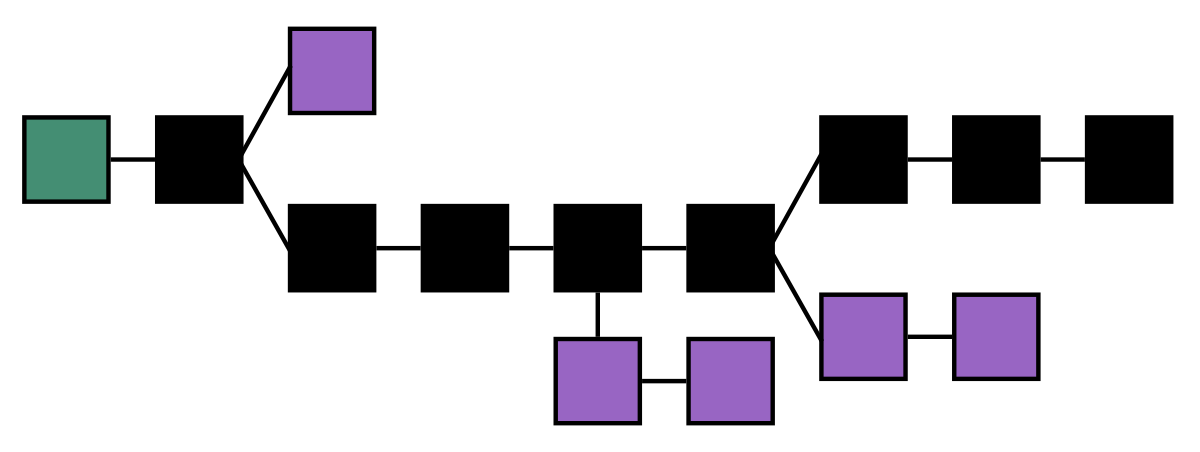
\includegraphics[width=\linewidth]{1.png}
	\caption{Ein Beispiel für eine Blockchain-Kette}
	\small \cite{first_image}
\end{figure} 


\section{Konstruktion des Blocks}
Ein Block speichert Informationen über Transaktionen, Zeitstempel, vorherigen Hash, Block-Hash.
\begin{itemize}
	\item \textbf{Magische Zahl :} Nummer, die diesen Block als Teil des Netzwerks einer bestimmten Kryptowährung identifiziert.
	\item \textbf{Transaktionen :} die Hauptinformationen und auch den größten Teil des Blocks
	\item \textbf{Transaktionszähler :} die Anzahl der im Block gespeicherten Transaktionen
	\item \textbf{Block Größe :} die maximale Größe der Informationen, die der Block enthält
\end{itemize} 
Ein Block enthält viele Informationen, belegt jedoch nicht viel Speicherplatz. Nehmen wir diese Elemente als Beispiel:
Was ist die Hauptinformationen, die ein Block (Transaktionen) enthält?
\begin{itemize}
	\item \textbf{Version:} Sie ist benutzbar, um einen neuen Block zu erstellen und um eine neue Version von Software zu identifizieren. Es ist auf 4 Bytes (4 x 8 „bits“) codiert.
	\item \textbf{Vorheriger Block-Hash:} Enthält einen Hash des Headers des vorherigen Blocks (md5, sha256 ...). Es ist auf 32 Bytes (32 x 8 = 256 „bits“) codiert.
	\item \textbf{Hash Merkle root:} Hash of transactions in the Merkle tree of the current block. Es ist auf 32 Bytes (32 x 8 = 256 „bits“) codiert.
	\item \textbf{Time:} Erstellungszeit des Blocks. Es ist auf 32 Bytes (32 x 8 „bits“) codiert.
	\item \textbf{Bits:} Es ist ein Wert, der die Schwierigkeitsbewertung des Ziel-Hashes und die Schwierigkeit beim Lösen der „Nonce“ angibt. Es ist auf 32 Bytes (32 x 8 „bits“) codiert.
	\item \textbf{Nonce:} Es ist die magische Zahl, die der Miner lösen muss, um einen Block im Blockchain-Netzwerk zu verifizieren und zu schließen.\\ \\
\end{itemize}

\textbf{Wichtige Anmerkung :} Die Miner setzen ihre Rechenleistung ein, um mithilfe von Zufallszahlen ( wie Bruteforce) die Nonce im Hash zu erraten. Sobald die Nonce erfolgreich bestimmt wurde, wird der Hash verifiziert und der Block geschlossen. Anschließend wird ein neuer Block mit einem Header erstellt und der Prozess wiederholt sich. Die Nonce ist von Interesse für Miner, da sie einen wichtigen Bestandteil des Mining-Prozesses darstellt, bei dem versucht wird, den Hash zu lösen. \\ \\ \\

\newpage
\subsubsection{Die Definition von Merkle-Bäumen}
Es handelt sich um eine Datenstruktur in Form eines Binärbaums, die in Bitcoin und Kryptowährung weit verbreitet ist und zur effizienten und sicheren Kodierung von Daten verwendet wird.

\section{Blockchaining-Mechanismus}
\textbf{Eine Blockchain funktioniert} ähnlich wie eine verkettete Liste, da sie aus einer Reihe von Blöcken besteht, die jeweils durch einen Hash des aktuellen Blocks und einen Hash des vorherigen Blocks miteinander verbunden sind. Dieser Mechanismus ermöglicht es, über die Kette zu iterieren, ähnlich wie bei einer verketteten Liste, bei der jeder Knoten einen Zeiger auf den vorherigen Knoten enthält.

\begin{figure}[h!]
	\centering
	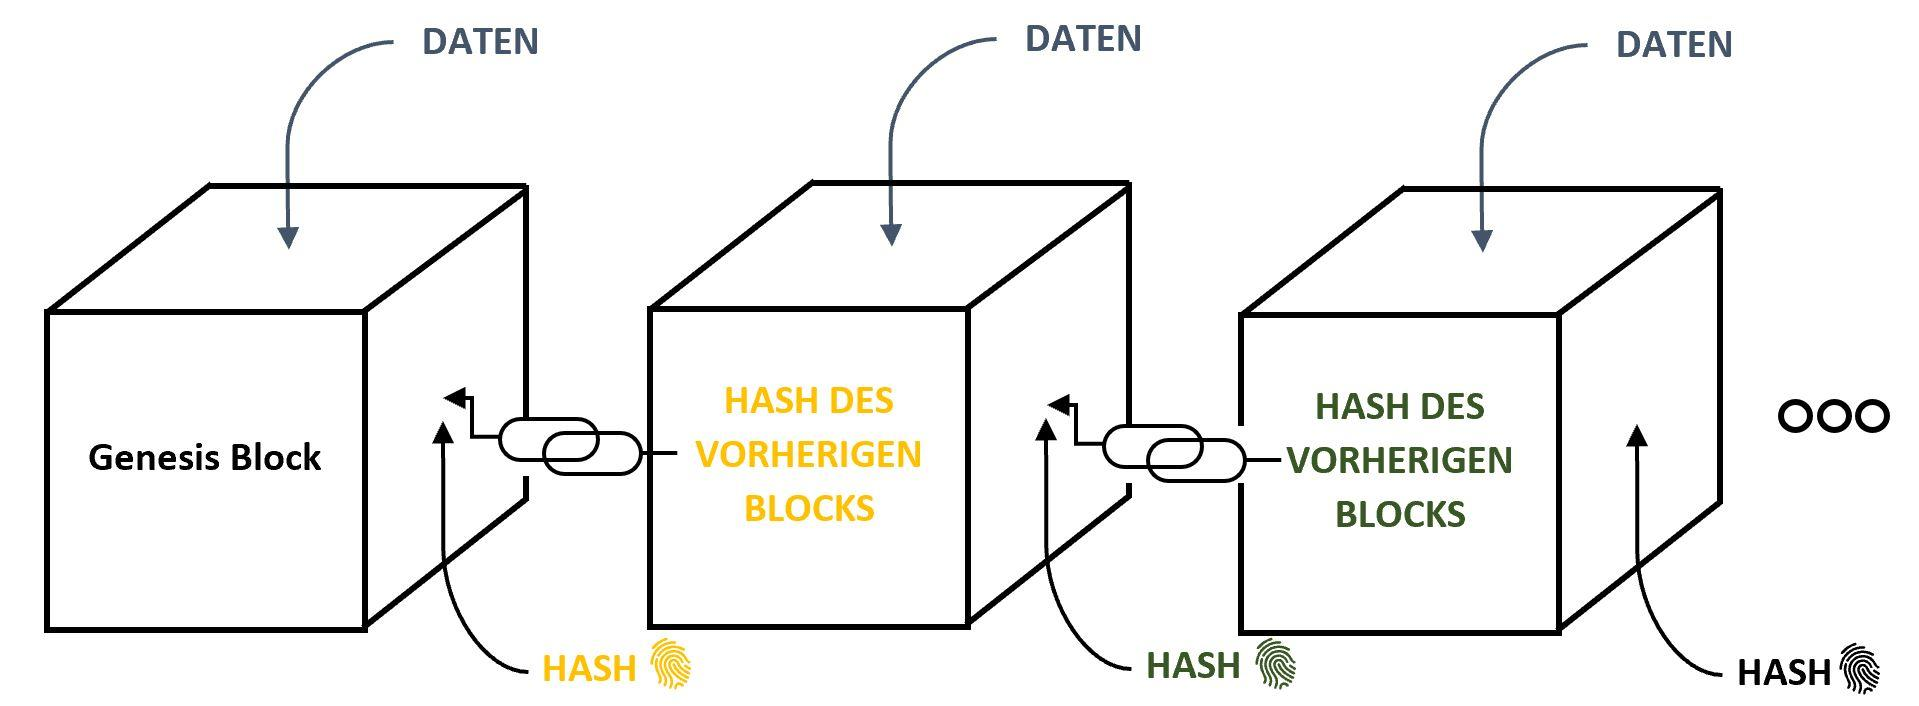
\includegraphics[width=\linewidth]{2.jpg}
	\caption{Der erste Block der Kette wird als Genius-Block bezeichnet.}
	\small \cite{seven_image}
\end{figure} 
In solchen Fällen sollte man immer im Hinterkopf behalten, dass Hacker versuchen werden, viele Angriffe auf das Blockchain-Netzwerk zu entwerfen, z. B. die Änderung oder Manipulation der Daten in Block (i). Dies führt zu einer Änderung des tatsächlichen Blocks i und macht das Feld "vorheriger Hash" in Block (i+1) ungültig. Das bedeutet, dass die Änderung eines Blocks alle nachfolgenden Blöcke in der Blockkette ungültig macht, was die Integrität der Kette beweist.\\
\textbf{Wichtige Anmerkung :} Die Verwendung von Hash reicht jedoch nicht aus, um verdächtige Manipulationen zu verhindern. Da Computer heute sehr schnell sind und Tausende von Hash-Operationen berechnen können, besteht technisch die Möglichkeit, einen Block zu manipulieren und alle Hashes der folgenden Blöcke neu zu berechnen, um das Netzwerk der Blockkette mit falschen Informationen wieder gültig zu machen. Aus diesem Grund verwendet die Bitcoin-Blockchain einen Konsensmechanismus, der als Proof-Of-Work (PoW) bezeichnet wird, um das Problem der Neuberechnung von Blöcken zu lösen. [ Diese Informationen sind von diesem Artikel und Buch genommen. \cite{imran2018mastering} und \cite{fool} ]

\section{Sicherung der Unveränderlichkeit und Zensurresistenz in Blockchain-Technologie}

Die Unveränderlichkeit und Zensurresistenz der Daten in einer Blockchain wird durch verschiedene Technologien und Mechanismen gewährleistet, darunter :

\begin{itemize}
	\item Konsensmechanismus
	\item Kryptografie
	\item Dezentralisierung
	\item Mehrere Kopien
\end{itemize} 
\subsection{Konsensmechanismus}\label{blockchain:konsensmechanismus}
Konsensmechanismus: ist ein Mechanismus, der es allen Teilnehmern einer Blockchain ermöglicht, Mining-Operationen durchzuführen, was bedeutet, komplexe mathematische Operationen zu lösen, um einen Block zu validieren und ihn der Hauptkette hinzuzufügen. In unserem Bericht haben wir ausschließlich über PoW berichtet. Es gibt verschiedene Beispiele dafür, z. B. \dq Proof-of-Work\dq, \dq Proof-of-Stake\dq oder \dq Proof-of-Space\dq.
\subsection{Kryptographische Methoden zur Datensicherung auf der Blockchain}
Kryptografie: Die Blockchain-Technologie nutzt Kryptografie, um Daten zu verschlüsseln und mit Hash-Funktionen wie SHA256, die von PoW verwendet werden, zu signieren. Dadurch wird die Sicherheit der Daten in der Blockchain gewährleistet, da jede Änderung an einer Transaktion oder einem Block sofort erkannt wird.
\subsection{Dezentralisierung}\label{blockchain:dezentralisierung}
Dezentralisierung: Eine Blockchain ist ein dezentralisiertes Netzwerk, das viele verschiedene Teilnehmer enthält. Das bedeutet, dass keine zentrale Behörde die Kontrolle über das Netzwerk hat, was es einer einzelnen böswilligen Person erschwert, die Daten zu verändern.
\subsection{Die Rolle von Mehrfachkopien bei der Datensicherung auf der Blockchain}\label{blockchain:kopien} 
Mehrere Kopien: Die Blockchain speichert mehrere Kopien ihrer Daten bei vielen verschiedenen Teilnehmern, was bedeutet, dass es schwieriger ist, alle Kopien einer Blockkette zu zensieren.

\section{Effizientes Mining durch Pooling: Eine Einführung in Mining-Pools}
Ein Mining-Pool ist eine Gruppe von Minern, die ihre Hardware kombinieren, um ihre Chancen auf Belohnungen durch den Prozess des Minings von Kryptowährungen zu erhöhen, die auf dem Proof-of-Work (PoW)-Konsensmechanismus basieren. Die kryptografischen Rätsel, die gelöst werden müssen, um Belohnungen zu erhalten, sind für einzelne Miner oft zu komplex zu lösen, und das Poolen von Ressourcen ermöglicht eine dynamischere Nutzung der Rechenleistung.  Der Mining-Pool ist dafür verantwortlich, die Verteilung der Belohnungen unter seinen Teilnehmern zu verwalten, was in der Regel automatisch geschieht, je nachdem, wie viel jeder Miner zur Lösung beigetragen hat, um den Hash zu finden.  Einige bekannte Mining-Pools im Jahr 2023 sind Antpool, BTCC Mining Pool und Slush Pool.

\begin{figure}[H]
	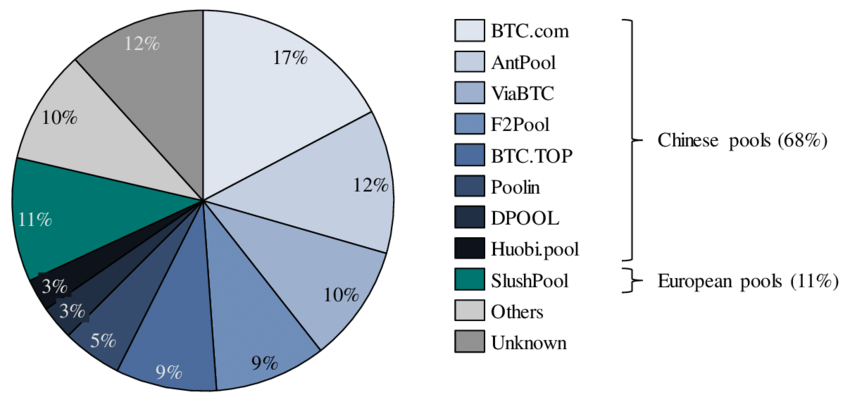
\includegraphics[width=\linewidth,height=8cm]{miningpool.png}
	\small{ \cite{second_image} }
\end{figure}




\chapter[Theoretische Seite der Proof-Of-Work-Methode]{Einführung in die „Proof-Of-Work“-Methode}	
\section{Einführung in die Proof-of-Work-Methode}
\subsection{Die Bedeutung der Methode in der Blockchain-Technologie}
\textbf{Proof-Of-Work} ist eine dezentrale Konsensmethode ( Der Konsensmechanismus wurde bereits in diesem Abschnitt in \cref{blockchain:konsensmechanismus} diskutiert.), bei der die Netzwerkteilnehmer Rechenleistung geben müssen, um ein Hash zu finden. Dieser Prozess dient als Abschreckung gegen Manipulation oder Ausbeutung des Systems, weil die Teilnehmer (Nodes) Arbeit leisten müssen. Was es ein sicheres Mittel zur Überprüfung der Integrität von Transaktionen und zur Aufrechterhaltung des Konsenses zwischen allen Mitgliedern des Netzwerks bietet.
\subsection{Proof-of-Work in der Blockchain-Technologie: Vorzüge und Empfehlungen für eine effektive Anwendung}
\textbf{Proof-Of-Work (POW)} wurde entwickelt, um zu verhindern, dass Nutzer Blocks in der Blockchain leicht manipulieren. Es verlangt von Minern, eine signifikante Menge an Mühe aufzuwenden, um einen Block zu erstellen. Diese Methode basiert auf verschiedenen Grundprinzipien in der Kryptowährung, wie folgt:

\begin{itemize}
	\item \textbf{Der Proof-Of-Work-Mechanismus sorgt dafür}, dass das Hinzufügen von Blöcken zur Blockchain-Kette mit einer gewissen Schwierigkeit verbunden ist, indem es Miner dazu zwingt, einen gültigen Hash zu finden. Diese Methode wurde so konzipiert, dass etwa alle zehn Minuten ein neuer Block mit einer festgelegten Menge an BTC in die Kette aufgenommen wird. Dies gewährleistet das algorithmische Wachstum der Geldmenge.
	\item \textbf{Die Verwendung von Proof-Of-Work} ermöglicht es den Nodes, die Integrität der Blockchain zu überprüfen, indem sie diejenige wählen, die den größten Aufwand in Form von Rechenleistung darstellt. Auf diese Weise ist es einfach zu erkennen, welche Blockchain die authentische ist.
	\item \textbf{Die Verwendung von Proof-Of-Work} dient dazu, das Blockchain-Netzwerk vor Angreifern zu schützen, da diese eine größere Energiemenge in das Netzwerk einspeisen müssten als alle anderen verfügbaren Miner insgesamt über einen längeren Zeitraum. Dies ist beim Bitcoin aufgrund der enormen Rechenleistung, die benötigt wird, um einen gültigen Block zu erstellen, praktisch unmöglich.
	\item \textbf{Proof-Of-Work ist eine bewährte Methode} zur Sicherung von Blockchains und zur Neuverteilung von digitalen Währungen. Im Gegensatz zu Fiatgeld, das von Zentralbanken gedruckt werden kann, erfordert die Erschaffung von Währungen in einem Proof-Of-Work-System einen tatsächlichen Einsatz von Ressourcen. Dadurch wird ein fairer Mechanismus für die Verteilung von Währungen gewährleistet.
\end{itemize}
\textbf{Anmerkung : } Die Informationen in diesem Abschnitt stammen aus der Quelle \cite{btc-echo-proof-of-work}.
\subsection{Sicherheit der Dezentralisierung im Proof-of-Work-Protokoll}
Die Dezentralität ( Die Dezentralisierung wurde bereits in diesem Abschnitt in \cref{blockchain:dezentralisierung} diskutiert. ) in dieser Methode ist abhängig von verschiedenen Faktoren,   der Verteilung der Mining-Ressourcen und der Zentralisierung der Mining-Pools. Wenn eine hohe Konzentration unter den Mining-Pools besteht, kann das zu einer kleineren Dezentralisierung führen, denn ein einzelner Mining-Pool könnte in der Lage sein, die Mehrheit der Rechenleistung des Netzwerks zu kontrollieren.
\subsection{Verbesserung der Dezentralisierung im Proof-of-Work-Protokoll}
Es gibt oft Maßnahmen wie die Förderung einer gleichmäßigen Verteilung der Mining-Ressourcen und die Einführung von Mechanismen, die eine Zentralisierung der Mining-Pools einschränken, ergriffen. Dies trägt zu einer fairen Verteilung der Rechenleistung bei und unterstützt außerdem den Aufbau eines robuster und sichereren Netzwerks.

\section{Proof-of-Work-Berechnungen in der Blockchain-Technologie}

\begin{description}
	\item[Hash-Funktion] Zuerst muss man wissen, wie die Hash-Funktion funktioniert, indem sie eine eindeutige, nicht invertierbare mathematische Funktion, die aus einer beliebigen Eingabestring eine feste Länge erzeugt. Sie könnte eine beliebig lange Zeichenfolge in eine eindeutige Zeichenfolge festgelegter Länge umwandeln. Beispiel hierfür ist der Einsatz der SHA-256-Hash-Funktion im Bereich des Minings.
	\item[Mining] ist ein Prozess, bei dem Miner versuchen, die Nonce und die Reihenfolge von jeden Parameter zu erraten, die von einer Hash-Funktion als Eingabe akzeptiert werden, um ein Ergebnis zu liefern. Da es unmöglich ist, die Hash-Funktion umzukehren, um die ursprüngliche Eingabe zu erhalten, müssen Miner eine Vielzahl (Milliarden von Berechnungen) von Operationen durchführen, um den Wert der Eingabe für die Hash-Funktion zu ermitteln. Sobald ein solches Ergebnis erzielt wurde, wird den Minern eine Belohnung gewährt.
\end{description}
\newpage
\subsubsection{Diese beschreiben den Prozess einer Transaktion im Blockchain-Netzwerk.}
\begin{enumerate}
	\item Die Blockchain generiert einen Block, der alle Transaktionen enthält, die in einem bestimmten Zeitraum stattgefunden haben.
	\item Der Verifizierer wird die Integrität der Transaktionen überprüfen, um sicherzustellen, dass sie legitim sind.
	\item Die Miner im Netzwerk überprüfen dann die Legitimität dieser Transaktionen und führen anschließend eine Suche durch, indem sie die Nonce und die Reihenfolge von jeden Parameter erraten. Der erfolgreiche Miner, der als erstes die Lösung findet, wird mit einer Belohnung(Anzahl von Bitcoins) bekommen.
	\item Das Blockchain-Netzwerk wird dann um den Block mit den bestätigten Transaktionen erweitert und wird als Teil der Blockchain gespeichert.
	\item Eine Transaktion wird als durchgeführt angesehen.
	\item Der Prozess wird wiederholt \\
\end{enumerate}
\subsubsection{Dies ist ein sequentielles Diagramm, das erklärt, wie es funktioniert}
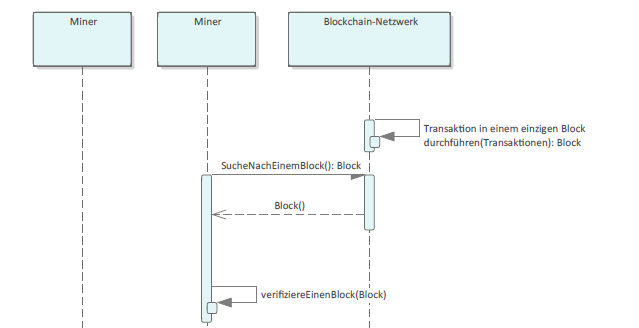
\includegraphics[width=\linewidth]{ProofOfWork1.png} \\ \\
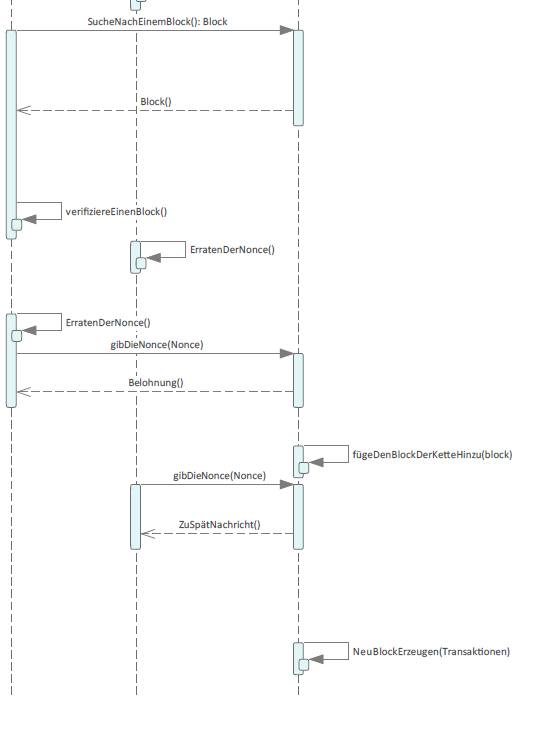
\includegraphics[width=\linewidth]{ProofOfWork2.png}

\section[Praktische Anwendung der Proof-Of-Work-Methode]{Algorithmus zur Bestimmung der Nonce in Kryptowährungen}
\begin{figure}[H]
	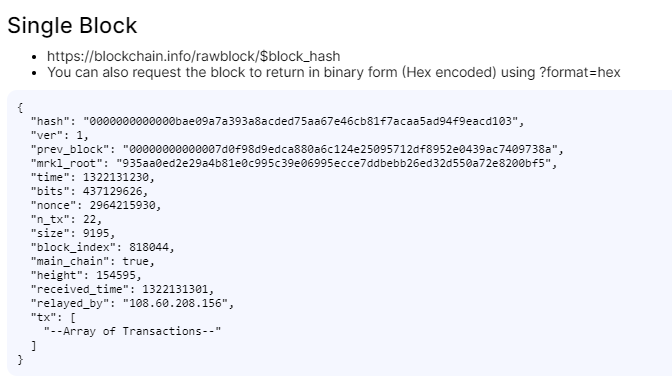
\includegraphics[width=\linewidth,height=8cm]{realblock.png}
	\small{ \cite{five_image} }
\end{figure}
Es ist von Interesse, die technische Funktionsweise von Proof-of-Work zu untersuchen. Als Erstes betrachten wir eine tatsächliche Blockstruktur von der offiziellen Website.
\begin{figure}[H]
	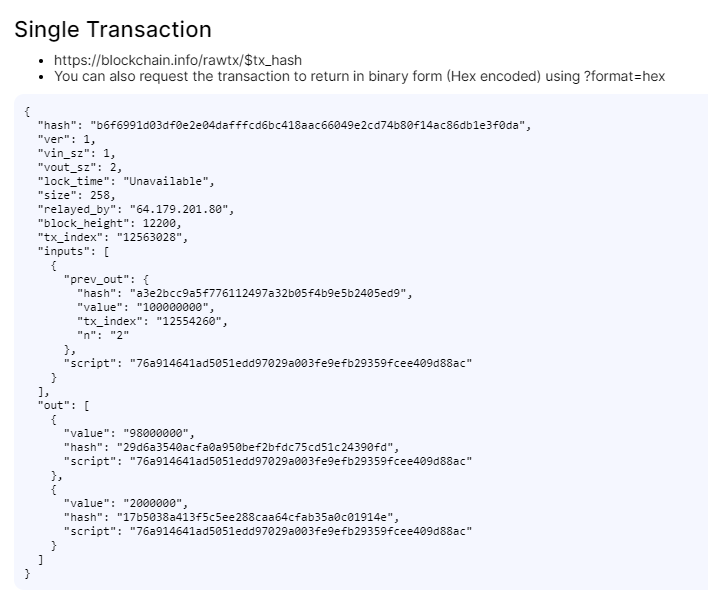
\includegraphics[width=\linewidth,height=10cm]{realtransaction.png}
	\caption{Die echten Blockchain-Block-Transaktionen.}
	\small{ \cite{five_image} }
\end{figure}
\begin{figure}[H]
	\centering
	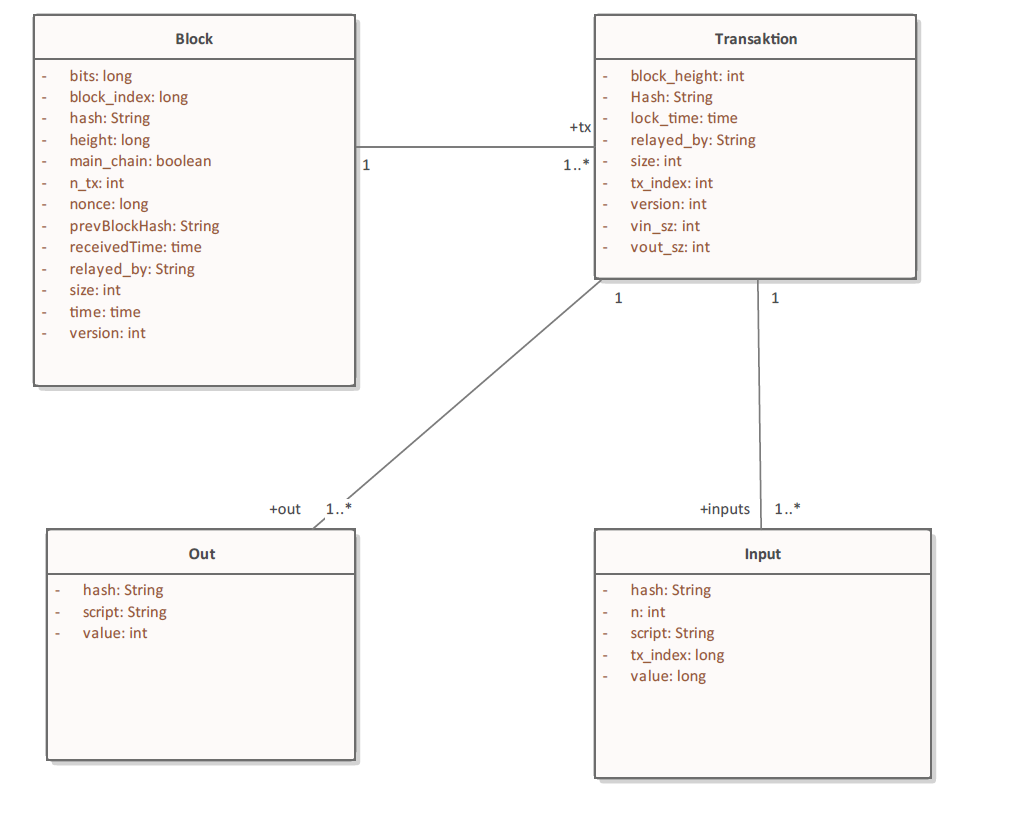
\includegraphics[width=\linewidth]{classOfStructures.png}
	\caption{Klassendiagram}
\end{figure}
Das nächste Diagramm, das als Klassendiagramm bezeichnet wird, gibt eine visuelle Darstellung aller Daten, die im realen Blockchain-Netzwerk enthalten sind. Dieses Diagramm ist hilfreich, um die Implementierung des Blockchain-Netzwerks besser zu verstehen und zu analysieren. Es zeigt die Beziehungen und Abhängigkeiten zwischen den verschiedenen Elementen des Netzwerks und hilft, die Struktur und Funktionsweise des Systems zu verdeutlichen. Die Verwendung eines Klassendiagramms ermöglicht es, die komplexen Zusammenhänge einfacher darzustellen und die Implementierung des Blockchain-Netzwerks besser zu verstehen.
\newpage
\begin{figure}[H]
	\centering
	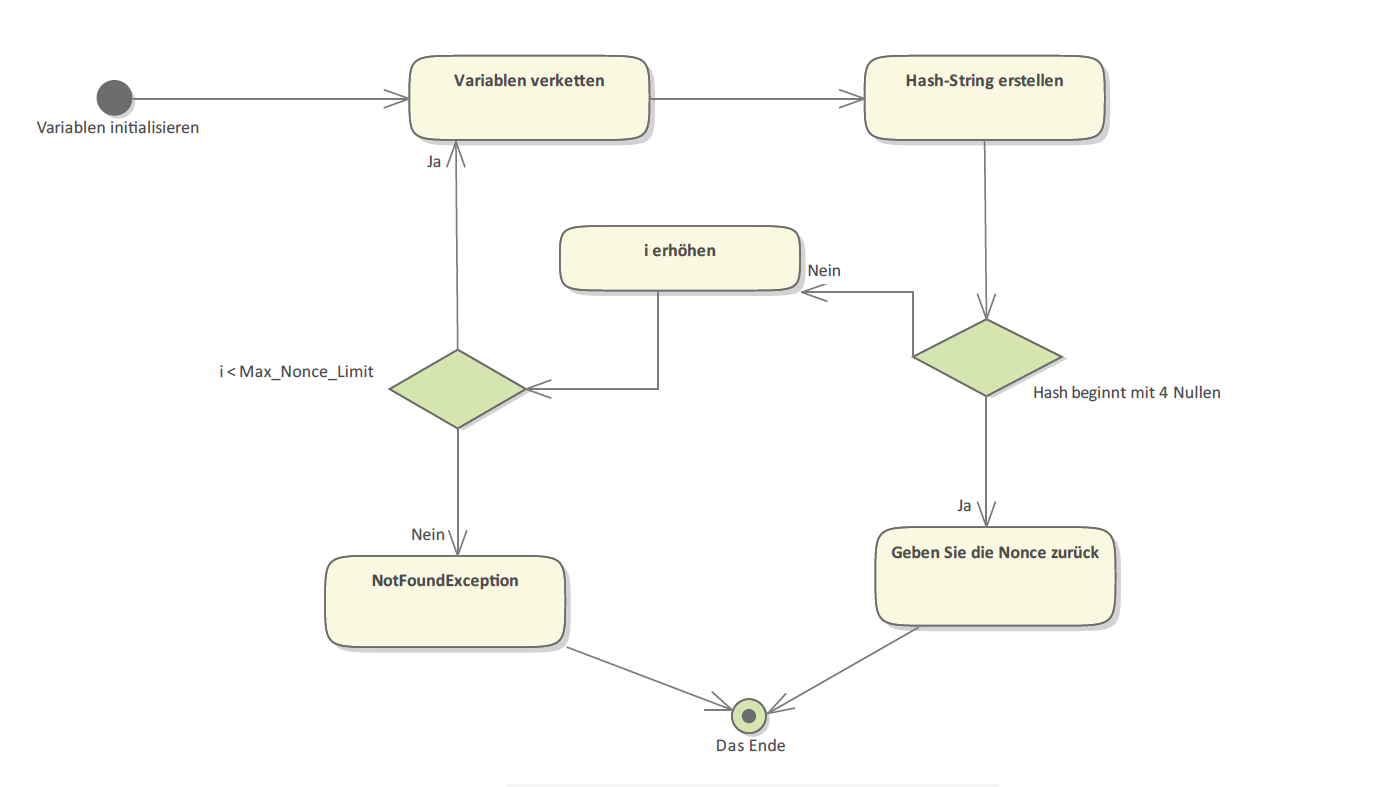
\includegraphics[width=\linewidth]{activity.png}
	\caption{Activity Diagram}
\end{figure}
Der Algorithmus zur Bestimmung der Nonce wird mit dem Aktivitätsdiagramm erklärt. Zunächst müssen wir die initialen Daten initialisieren, einschließlich des MaxNonceLimit, der Anzahl der Nullen, die der Hash haben sollte. In diesem Beispiel betrachten wir die Anforderung, dass der Hash mit 4 Nullen beginnen sollte. Es ist wichtig zu beachten, dass die Anzahl der Nullen eine wichtige Rolle bei der Bestimmung der Komplexität des Algorithmus spielt. Je höher die Anzahl der Nullen, desto länger wird es dauern, die Nonce mit begrenzter Hardware zu finden. Wir sollten auch unsere Inkrementierungsvariable für die for-Schleife initialisieren.
\textbf{Dies ist der Algorithmus \textcommabelow der für dieses Beispiel zum Schürfen von Bitcoin geschrieben wurde} \\
\begin{algorithm}
	\caption{Nonce für gültigen Hash finden}
	\label{alg:nonce_find}
	
	\begin{algorithmic}[1]
		\State nonce $\gets$ 0
		\Repeat
		\State hash $\gets$ Hash(block\_data, nonce)
		\If{hash meets difficulty level}
		\State \textbf{return} nonce
		\EndIf
		\State nonce $\gets$ nonce + 1
		\Until{hash meets difficulty level}
	\end{algorithmic}
\end{algorithm}

\section{Vor- und Nachteile von Proof-Of-Work}
\textbf{Um die Vor- und Nachteile dieser Methode genau zu erklären, wurde diese Tabelle erstellt : }  \\
\begin{tabular}{|c|c|}
	\hline
	\textbf{Vorteile} & \textbf{Nachteile} \\ \hline
	Sicherheit & Hohe Energiekosten \\ \hline
	Gute Anreizstruktur & Langsame Transaktionsgeschwindigkeiten \\ \hline
	Breite Akzeptanz & Mögliche Zentralisierung von Mining-Pools \\ \hline
	Verteilte Konsensfindung & Hardware-Anforderungen \\ \hline
\end{tabular}\\ \\
\textbf{\underline{Eklärung :}}
\begin{itemize}
	\item \textbf{Sicherheit :} Um ein hohes Maß an Sicherheit in einem auf Proof-Of-Work basierenden Blockchain-Netzwerk zu gewährleisten, müsste eine spekulative Person nicht die Kontrolle über den größten Teil der Mining-Kapazität übernehmen. Dies würde bedeuten, mindestens 50\% des Netzwerks zu besitzen, was aufgrund der verteilten Natur von Proof-of-Work-Systemen als unmöglich angesehen wird. Eine solche Person würde auch eine große Menge an Hardware und Energie benötigen, um die notwendige Rechenleistung erbringen zu können.
	
	
	\item \textbf{Gute Anreizstruktur :} Eine gute durchdachte Anreizstruktur ist ein wesentlicher Faktor für den Erfolg eines Proof-of-Work-Systems. Die Miner erhalten eine finanzielle Belohnung für das Lösen von Rechenproblemen und die damit verbundenen Anstrengungen, was sie dazu veranlasst, ihre Rechenleistung (z.B : mit Rig Mining"-Geräte ) zur Verfügung zu stellen, um auf diese Weise die Integrität und Sicherheit der Blockchain zu gewährleisten. Dies bedeutet, dass eine gute Anreizstruktur auch dazu beitragen kann, das System im Gleichgewicht zu halten und die Teilnahme der Miner zu fördern. Wenn die Belohnungen für das Mining zu niedrig sind, könnten die Miner weniger motiviert sein, ihre Rechenleistung zur Verfügung zu stellen, denn manchmal, wenn die Belohnung zu niedrig ist, wird dies nicht die Stromkosten für die Mining-Operationen bezahlen, folglich könnte die Sicherheit darunter leiden. Andererseits könnten zu hohe Belohnungen dazu führen, dass das System aus dem Gleichgewicht gerät und die Mining-Pools zentralisiert werden. Es ist wichtig, dass die Anreizstruktur von Proof-of-Work-Systemen sorgfältig angepasst wird, um eine ausgewogene Beteiligung der Miner und ein hohes Sicherheitsniveau zu gewährleisten.
	
	
	\item \textbf{Breite Akzeptanz :} PoW wird in der Kryptowährungsgemeinschaft weitgehend akzeptiert, da diese Methode ein hohes Maß an Sicherheit sowie Integration und Dezentralisierung bietet.
	
	\item \textbf{Verteilte Konsensfindung :} Die dezentralisierte Konsensbildung, die hier in [ \cref{blockchain:dezentralisierung} ] erklärt ist ein wichtiger Aspekt von Blockchain-Systemen. \\
\end{itemize}
\textbf{Obwohl der Proof-of-Work ein wichtiger Konsensmechanismus in vielen Kryptowährungen ist, gibt es auch einige Nachteile, die berücksichtigt werden sollten.}
\begin{itemize}
	\item \textbf{Hohe Energiekosten :} Der Betrieb eines Proof-of-Work-Blockchain-Netzwerks kann energieintensiv sein, da die Miner Rechenleistung aufbringen müssen, um neue Blöcke zu erzeugen und Transaktionen zu validieren. Dies erfordert ständig den Einsatz von speziellen Mining-Geräten, die viel Energie verbrauchen und möglicherweise auch Kühlsysteme benötigen, um hohe Temperaturen zu vermeiden. Eine Möglichkeit, den Energiebedarf des Mining-Betriebs zu senken, besteht darin, erneuerbare Energien zur Erzeugung des wichtigen Stroms zu nutzen. Dies kann zwar eine größere Anfangsinvestition erfordern, bietet aber auch langfristige Vorteile, da die Mining-Unternehmen keinen externen Strom verbrauchen und somit keine Energiekosten anfallen. Erneuerbare Energien wie Solar- und Windenergie können eine umweltfreundliche Alternative zu fossilen Brennstoffen bieten.
	
	\item \textbf{Langsame Transaktionsgeschwindigkeiten :} Eines der Haupthindernisse für die Geschwindigkeit von Bitcoin-Transaktionen ist die Tatsache, dass sie von Minern validiert werden müssen, um in die Blockchain aufgenommen zu werden. Da die Schwierigkeit, einen neuen Block zu finden, von Zeit zu Zeit angepasst wird, kann es durchaus einige Zeit dauern, bis ein Block gefunden wird. Die durchschnittliche Zeit, die benötigt wird, um einen neuen Block zu finden, beträgt derzeit etwa 10 Minuten. Das bedeutet, dass es normalerweise etwa 10 Minuten dauert, bis eine Transaktion bestätigt und in die Blockchain eingetragen wird. Für einige Nutzer mag dies als langsam empfunden werden, insbesondere im Vergleich zu herkömmlichen Zahlungsmethoden. Es gibt jedoch Maßnahmen, die die Geschwindigkeit von Bitcoin-Transaktionen verbessern können, wie z. B. die Verwendung von SegWit (Segregated Witness) oder Lightning-Netzwerken. Diese Technologien können die Größe der Transaktionen verringern und somit ihre Geschwindigkeit erhöhen.
	\begin{figure}[H]
		\centering
		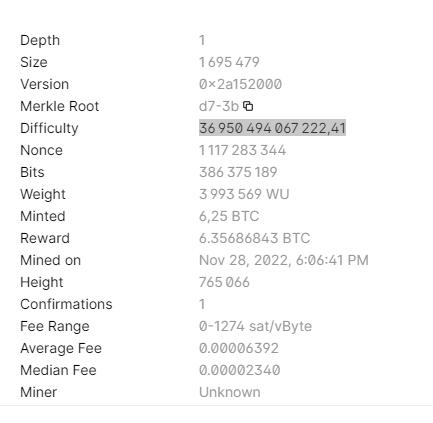
\includegraphics[width=7cm,height=7cm]{difficulty}
		\caption{Die heutige Schwierigkeit ist}
		\small \cite{five_image}
	\end{figure} 
	
	\item \textbf{Mögliche Zentralisierung von Mining-Pools :} Proof-of-Work-Mining-Pools können zentralisiert werden, wenn einige wenige große Mining-Pools einen Hauptteil der Blockgenerierungsrate kontrollieren und damit Kontrolle über das Netzwerk ausüben können.  Dies kann zu einer Verletzung der Dezentralisierung und der Netzwerksicherheit führen, wenn diese Pools die Macht haben, das Netzwerk zu beeinflussen oder anzugreifen.
	
	\item \textbf{Hardware-Anforderungen :} Das Bitcoin-Mining kann hohe Investitionskosten erfordern, da oftmals spezielle Mining-Hardware wie leistungsstarke Grafikkarten, entsprechende Motherboards oder sogar die Erstellung von Rig-Computern notwendig sind, um erfolgreich neue Blöcke zu erzeugen. Der hohe Preis dieser Hardware kann den Einstieg in das Bitcoin-Mining hingegen für Gruppen oder kleine Unternehmen schwierig machen. Dennoch kann das Bitcoin-Mining lukrativ sein, vor allem für große Mining-Unternehmen, die über mehrere Mining-Anlagen verfügen und Zugang zu billigem Strom haben. In diesen Fällen können die Einnahmen aus dem Mining die Investitionskosten schnell übersteigen und eine profitable Einnahmequelle darstellen.
	
\end{itemize}

\textbf{Anmerkung : } Die Informationen in diesem Abschnitt stammen aus dem Artikel \cite{fool} und diesem Buch \cite{kube2018daniel}.
%%%%%%%%%%%%%%%%%%%%%%%%%%%%%%%%%%%%%%%%%%%%%%%%%%%%%%%%%%%%%%%%%%%%%%%%%%%%%%
%%%%%%%%%%%%%%%%%%       Schwierigkeit und Schwierigkeit        %%%%%%%%%%%%%%
%%%%%%%%%%%%%%%%%%%%%%%%%%%%%%%%%%%%%%%%%%%%%%%%%%%%%%%%%%%%%%%%%%%%%%%%%%%%%%
\chapter{Schwierigkeit und Sicherheit des Proof-Of-Work}

\section{Die Bedeutung der Schwierigkeit im Proof-of-Work-Protokoll}
\begin{itemize}
	\item Die Schwierigkeit besteht darin, die gewünschte Hash-Ausgabe zu finden. Zum Beispiel Bitcoin, es wird eine Frage gestellt: Wie viele Nullen soll die Ausgabe am Anfang des Strings haben. Je mehr Nullen gefordert sind, desto schwieriger wird es schließlich, den Output zu finden.
	\item Die Schwierigkeit ist bei Bitcoin immer so gewählt, dass im Schnitt alle zehn Minuten ein neuer Block gefunden werden soll. Dieser Benchmark wird alle zwei Wochen überprüft. Stellt sich heraus, dass in zwei Wochen der Richtwert von 2.016 Blöcken überschritten wurde, also mehr Blöcke als gewünscht gefunden wurden, ist die Schwierigkeit zu gering und wird nach oben korrigiert – und umgekehrt.
\end{itemize}
%

\section{Schwierigkeitsanpassung im Proof-of-Work-Protokoll der Blockchain-Technologie}
\textbf{Anmerkung :} Die folgende Informationen stammen aus diesem Buch \cite{lewis2018basics}.
\begin{itemize}
	\item Die Schwierigkeit eines PoW kann angepasst werden, um sicherzustellen, dass die Blockerzeugungsrate stabil bleibt. In einem PoW-System werden Miner ausgewählt, um einen neuen Block mit PoW zu erstellen. Wenn viele Miner am Netzwerk beteiligt sind, werden die Blöcke schneller erstellt, was zu einer Erhöhung der Blockerzeugungsrate führt. Wenn hingegen nur wenige Miner am Netzwerk teilnehmen, werden die Blöcke sehr langsam erstellt, was zu einer Abnahme der Blockerzeugungsrate führt. Um die Stabilität der Blockerzeugungsrate zu behalten, wird eine Technologie zur Anpassung der Schwierigkeit verwendet, die in Englisch "Difficulty Adjustment Algorithm (DAA)" heißt. Diese Implementierung ist spezifisch für jede verwendete Kryptowährung, aber ihr Konzept besteht darin, die Schwierigkeit auf dynamische Weise anzupassen. 
	
	\item Das Konzept dieses Algorithmus besteht darin, die Schwierigkeit so anzupassen, dass die für die Erstellung eines neuen Blocks erforderliche Zeit konstant bleibt. Diese Änderung der Schwierigkeit wird für jeden Block dynamisch angepasst, abhängig von der Zeit, die für die Erstellung des vorherigen Blocks benötigt wurde. Wenn ein Block schneller als erwartet erstellt wurde, wird die Schwierigkeit erhöht, um die Blockerstellungsrate zu verlangsamen. Falls ein Block langsamer erstellt wurde, wird die Schwierigkeit verringert, um die Blockerstellungsrate zu beschleunigen. Beachten Sie, dass die aktuelle Schwierigkeit der Blockerstellung in der Blockchain 10 Minuten ist. Dabei hilft die Verwendung von DAA diese Schwierigkeit konstant zu behalten.
\end{itemize}
\subsection{Auswirkungen einer zu niedrigen Schwierigkeitseinstellung im Proof-of-Work-Protokoll}
Wenn die PoW Difficulty zu niedrig eingestellt ist, kann dies zu Instabilitäts- und Integritätsproblemen, Sicherheitsproblemen und auch wirtschaftlichen Problemen führen:
Sehr hohe Blockgenerierungsrate: Miner können schnell Blöcke erstellen, was zu einer höheren Blockgenerierungsrate führt, da die Schwierigkeit niedrig ist, was manchmal zu einer Überlastung des Netzwerks und einer langsameren Verarbeitung von Transaktionen führt.
Sicherheitsprobleme: Ein niedriger Schwierigkeitsgrad macht das Netzwerk anfällig für 51\%-Angriffe, bei denen ein Angreifer die Mehrheit der Mining-Kapazität nutzen und das Netzwerk mit leistungsstarker Hardware manipulieren kann. 
Wirtschaftliche Probleme: Wenn Blöcke schneller erzeugt werden, kann dies zu einem schnellen Drucken führen, da Kryptowährungen gedruckt werden. Dies kann den Wert der Kryptowährung verringern.
\subsection{Auswirkungen von Schwierigkeitsgrad und Netzwerkgröße auf die Sicherheit und Integrität der Blockchain-Technologie im Proof-of-Work-Protokoll}
Der Schwierigkeitsgrad des Proof of Work (PoW) und die Größe des Netzwerks haben einen erheblichen Einfluss auf die Sicherheit und Integrität der Blockchain.
\begin{description}
	\item[PoW-Schwierigkeit : ] Die PoW-Schwierigkeit bestimmt das Verhältnis zwischen der Zeit und der Anzahl der Berechnungen, die zur Lösung eines neuen Blocks erforderlich sind. Je höher der Schwierigkeitsgrad, desto mehr Rechenleistung ist für die Lösung des Blocks erforderlich. Diese zusätzliche Rechenleistung macht das Netzwerk sicherer, da es für einen Angreifer schwieriger ist, genügend Mining-Power zu haben, um seinen 51\%-Angriff auszuführen.
	\item[Größe des Netzwerks : ] Ein großes Netzwerk bedeutet mehr Mining-Kapazität und eine bessere Verteilung der Verarbeitungsleistung, wodurch das Netzwerk sicherer wird. Größere Netzwerke sind auch weniger anfällig für 51\%-Angriffe, da Angreifer mehr Mining-Kapazität benötigen, um ihre Angriffe zu starten.
\end{description}
Die Beziehung zwischen diesen beiden Begriffen besteht darin, dass sie beide zur Verbesserung der Sicherheit und Integrität von Blockchains beitragen. Eine angemessene PoW-Schwierigkeit hält das Netzwerk zu 51\% sicher vor Angriffen, während ein größeres Netzwerk eine bessere Verteilung der Mining-Kapazität gewährleistet und das Netzwerk insgesamt stabiler macht. 


%%%%%%%%%%%%%%%%%%%%%%%%%%%%%%%%%%%%%%%%%%%%%%%%%%%%%%%%%%%%%%%%%%%%%%%%%%%%%%
%%%%%%%%%%%%%%%%%%       Sidechains                             %%%%%%%%%%%%%%
%%%%%%%%%%%%%%%%%%%%%%%%%%%%%%%%%%%%%%%%%%%%%%%%%%%%%%%%%%%%%%%%%%%%%%%%%%%%%%

\chapter{Sidechains}
Am 22. Oktober 2014 wurde die Idee einer Sidechain in einem bahnbrechenden wissenschaftlichen Dokument vorgestellt. Das Dokument wurde von Adam Back, dem Schöpfer von HashCash und CEO von Blockstream, und einer Gruppe führender Bitcoin-Ingenieure verfasst, darunter Matt Corallo, Luke Dashjr und Mark Friedenbach, Mitbegründer von Blockstream. \cite{coin_desk}\\ \\
Diese Autoren spielten eine wichtige Rolle bei der Entwicklung von Satoshi Nakamotos Vision eines elektronischen Währungssystems, indem sie den Proof-of-Work-Konsensmechanismus von HashCash in die Bitcoin-Blockchain integrierten. Sie räumten jedoch ein, dass es noch Raum für Verbesserungen gab, wenn Bitcoin ein weltweites Publikum bedienen sollte. \\ \\
Zu dieser Zeit stand die Bitcoin-Infrastruktur vor Herausforderungen wie Kompromissen zwischen Skalierbarkeit und Dezentralisierung sowie Bedenken hinsichtlich Datenschutz und Zensur. Um diesen Herausforderungen zu begegnen, schlugen die Autoren eine neue Technologie namens "pegged sidechains" vor, die es ermöglichen würde, Bitcoins und andere Ledger-Assets zwischen mehreren Blockchains zu transferieren. Dies würde den Nutzern den Zugang zu neuen und innovativen Kryptowährungssystemen ermöglichen, indem sie die Vermögenswerte nutzen, die sie bereits besitzen.\\ \\
Das Weißbuch zu Seitenketten hat eine revolutionäre Lösung für die Beschränkungen der Bitcoin-Infrastruktur vorgestellt und die Grundlage für neue Entwicklungen in der Welt der Blockchain-Technologie geschaffen.

\section{Sidechain : Eine Analyse der Definition und Eigenschaften}
\subsection{Definition von Sidechain}
Die Sidechains der Blockchain werden als separate Blockchains behandelt, die mit der Hauptblockchain verbunden sind. Diese Beziehung zwischen ihnen ermöglicht den Austausch und die Überprüfung von Daten auf die gleiche Weise wie bei der Hauptblockkette. Sidechains bieten in der Regel nicht die gleiche Sicherheit und Skalierbarkeit wie ihre Hauptblockchain. Das liegt daran, dass es weniger Knoten gibt und somit weniger Ressourcen benötigt werden. Daher sollte die Verwendung von Sidechains gut abgewogen werden. 
\subsection{Sidechain, auf die Proof-Of-Work basieren}
Die Sidechains der Blockchain werden durch PoW verifiziert. Das bedeutet, dass die Sidechain-Knoten eine bestimmte Anzahl von Ressourcen benötigen, um die Integrität des Netzwerks zu gewährleisten und Transaktionen zu bestätigen. Allerdings kann die Schwierigkeit der PoW für Sidechains und Mainchains unterschiedlich oder gleich sein, je nach den spezifischen Anforderungen und Einschränkungen der Sidechains.
\subsection{Eigenschaften}
Eine Sidechain ist ein einzelnes Blockchain-Netzwerk, das über eine bidirektionale Verbindung mit einer anderen Blockchain, dem sogenannten Mainnet oder der übergeordneten Blockchain (hier wird alles in \cref{blockchain:definition} beschrieben), verbunden ist. Diese sekundäre Blockchain hat ihren eigenen Satz von Konsensprotokollen, was den Datenschutz und die Sicherheit verbessert und den Bedarf an Vertrauen verringert. \\\\
Einer der Hauptvorteile von Sidechains ist die Möglichkeit des einfachen Austauschs von Vermögenswerten zwischen dem Mainnet und der sekundären Blockchain. Dadurch können digitale Vermögenswerte wie Token sicher von einer Blockchain auf eine andere übertragen werden, was Projekten neue Möglichkeiten eröffnet, ihr Ökosystem auf dezentrale Weise zu erweitern. \\ \\
Nehmen wir an, Sie haben einige Bitcoin im Haupt-Bitcoin-Netzwerk. Um Ihre Bitcoin auf eine Sidechain zu verschieben, senden Sie sie an eine bestimmte Ausgabeadresse. Diese Adresse könnte eine Hardware-Wallet, eine Hot-Wallet oder eine Sidechain sein. Sobald die Transaktion bestätigt ist, wird sie über das Bitcoin-Netzwerk verbreitet. \\ \\
Nach einer kurzen Sicherheitsprüfung wird der Bitcoin auf die Sidechain übertragen, so dass Sie Ihr Vermögen in das neue Netzwerk verschieben können. Dieser Prozess ermöglicht einen nahtlosen Übergang von Vermögenswerten zwischen verschiedenen Blockchain-Netzwerken und bietet den Nutzern mehr Optionen und Flexibilität.\\
\textbf{Anmerkung : } Die Informationen in diesem Abschnitt stammen aus der Quelle \cite{coin_desk}.

\textbf{Obwohl das Konzept der Seitenketten einfach zu sein scheint, gibt es eine Reihe entscheidender Elemente, die notwendig sind, damit sie optimal funktionieren. Zu diesen wesentlichen Komponenten gehören:}

\begin{itemize}
	\item Two-way peg
	\item Intelligente Verträge
\end{itemize}


\begin{figure}[H]
	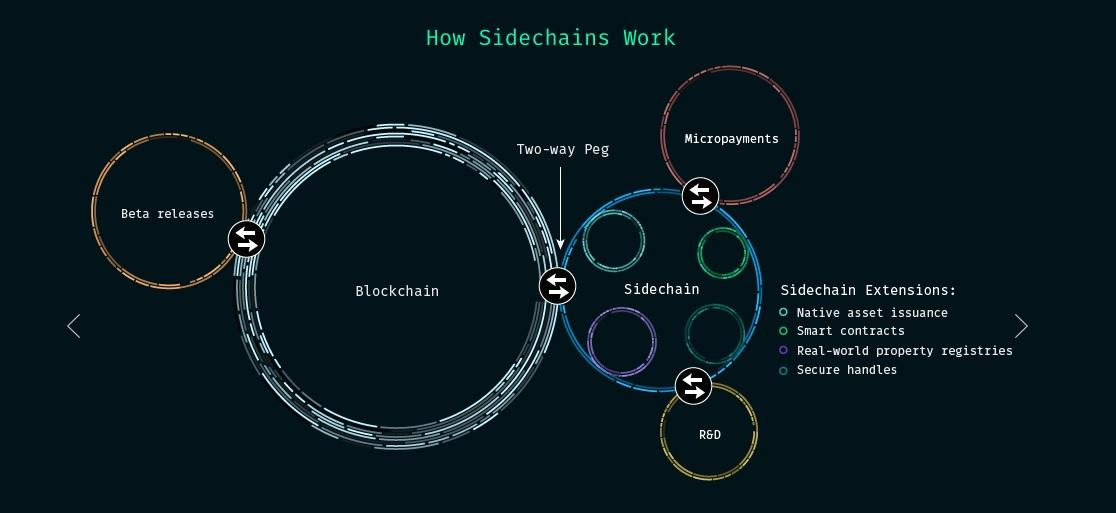
\includegraphics[width=\linewidth,height=6cm]{sidechain}
	\caption{Mechanismus der Sidechain}
	\small{ \cite{third_image} }
\end{figure}

\section{Two-way peg}
Sidechains wurden geschaffen, um eine nahtlose Übertragung von digitalen Vermögenswerten zwischen verschiedenen Blockchains zu ermöglichen, unabhängig davon, wer sie besitzt. Diese Übertragung sollte ohne die Möglichkeit der Beeinflussung durch eine dritte Partei erfolgen. Um dies zu erreichen, wird ein Zwei-Wege-Peg benötigt, den man sich wie einen Zwei-Wege-Tunnel vorstellen kann, der die beiden Blockchains miteinander verbindet. \\

\begin{figure}[H]
	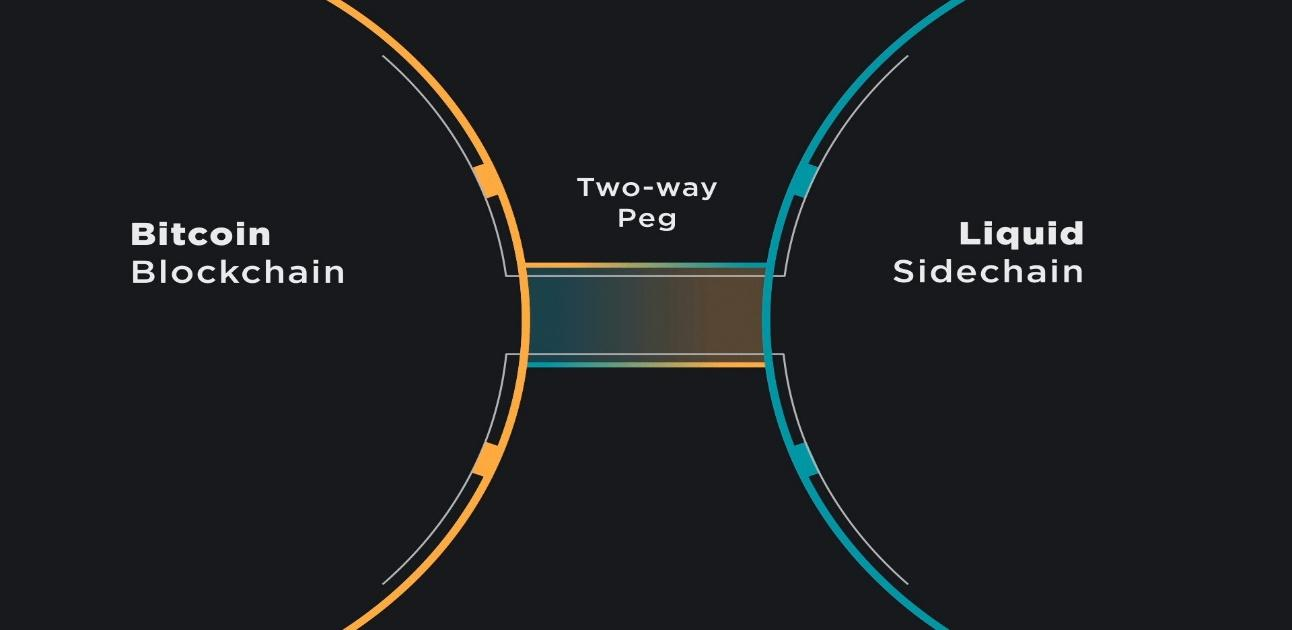
\includegraphics[width=\linewidth,height=6cm]{twowaypeg}
	\caption{Two way peg}
	\small{\cite{six_image}}
\end{figure}

Laut dem Sidechain-Whitepaper (“The mechanism by which coins are transferred between sidechains […] a pegged sidechain is a sidechain whose assets can be imported from and returned to other chains.” [ die Quelle davon ist im Literaturverzeichnis als \cite{blockstream2014enabling} zu finden ]) bezieht sich ein Zwei-Wege-Peg auf die Methode, mit der digitale Vermögenswerte wie Bitcoin zwischen der Hauptblockchain und der neuen Sidechain hin und her übertragen werden können. Wichtig ist, dass die Übertragung von Vermögenswerten nicht tatsächlich stattfindet. Stattdessen werden die Vermögenswerte auf der Hauptblockchain gesperrt, während der entsprechende Wert auf der Sidechain freigegeben wird. \\ 
Dies setzt das Vertrauen voraus, dass die Teilnehmer oder "Validierer", die an dem wechselseitigen Pflock beteiligt sind, ehrlich handeln. Andernfalls könnte es zu betrügerischen Überweisungen kommen oder legitime Überweisungen könnten blockiert werden.
\section{Intelligente Verträge}
Um digitale Vermögenswerte von einem Mainnet auf eine Sidechain oder umgekehrt zu übertragen, ist ein Prozess erforderlich, der außerhalb des Haupt-Blockchain-Netzwerks stattfindet und Informationen zwischen den beiden Blockchains überträgt. Dieser Prozess, der als Off-Chain bezeichnet wird, beinhaltet einen intelligenten Vertrag, der sicherstellt, dass die Übertragung von digitalen Vermögenswerten fair und sicher ist.
Wenn eine Transaktion stattfindet, bestätigt der intelligente Vertrag diese und benachrichtigt das Hauptnetz. Anschließend sendet der Off-Chain-Prozess die Transaktionsdetails an einen intelligenten Vertrag auf der Sidechain, wo sie überprüft werden. Nach der Verifizierung werden die digitalen Vermögenswerte auf der Sidechain freigeschaltet, so dass sie frei zwischen den beiden Blockchains bewegt werden können.
Intelligente Verträge spielen eine wichtige Rolle bei der Gewährleistung der Sicherheit dieser Transaktionen, da sie die Teilnehmer sowohl im Mainnet als auch auf der Sidechain zu ehrlichem Handeln verpflichten. Durch ein sicheres Verfahren können digitale Vermögenswerte zwischen den Blockchains übertragen werden, ohne dass das Risiko eines Fehlverhaltens besteht. [ Diese Informationen sind aus diesem Buch \cite{imran2018mastering} übernommen ].

\begin{figure}[H]
	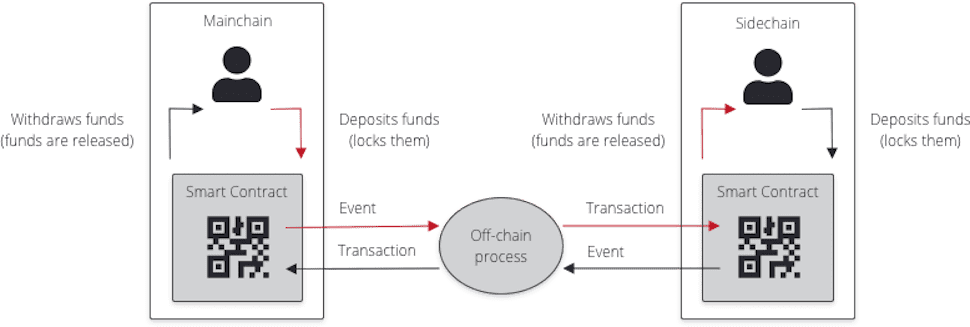
\includegraphics[width=\linewidth,height=6cm]{contracts}
	\caption{Intelligente Verträge}
	\small{ \cite{four_image} }
\end{figure}

\section{Sidechain bei Bitcoin}
Beispiele für praktische Sidechain-Anwendungen sind das Liquid Network und RootStock (RSK). Beide Sidechains sind mit dem Bitcoin-Mainnet verbunden und können nur für Aktivitäten im Zusammenhang mit Bitcoin genutzt werden. \\
Das Liquid Network, eine von Blockstream entwickelte Open-Source-Sidechain, baut auf dem Bitcoin-Mainnet auf. Die schnelle Blockentdeckungszeit von einer Minute im Vergleich zu 10 Minuten bei Bitcoin ermöglicht es, 10 Mal mehr Blöcke zu seiner Sidechain hinzuzufügen. Darüber hinaus bietet das Netzwerk einen verbesserten Datenschutz, indem es die Menge und die Art der übertragenen digitalen Vermögenswerte verbirgt.\\
RSK hingegen ist eine Sidechain, die speziell für die Unterstützung intelligenter Verträge entwickelt wurde. Bei der Verwendung von RSK wird Bitcoin vorübergehend im Mainnet gesperrt und als RSK-eigene Währung, Smart Bitcoin (SBTC), freigegeben.
Aufgrund seiner Smart-Contract-Fähigkeiten müssen Nutzer ihre Bitcoin nicht in andere Vermögenswerte umwandeln, um Smart Contracts zu nutzen, was es mit anderen Blockchain-Netzwerken wie Ethereum interoperabel macht. [ Diese Informationen sind aus diesem Artikel \cite{coin_desk} übernommen ] \\

\subsubsection{Prozess der Sidechain bei Proof of work}

\begin{enumerate}
	\item Die Übertragung von digitalen Assets von der Hauptkette zur Sidechain wird gestartet.
	\item Das digitale Asset wird an eine spezielle Ausgabeadresse auf der Hauptkette gesendet.
	\item Die Übertragung wird bestätigt und auf beiden Blockchains dokumentiert.
	\item Die Bestätigung wird über das Netzwerk der Hauptkette verbreitet.
	\item Nach einer Sicherheitsprüfung wird das digitale Asset auf die Sidechain transferiert.
	\item In der Sidechain wird das digitale Asset in einem Block gespeichert und über das Netzwerk verbreitet.
	\item Das digitale Asset ist jetzt auf der Sidechain verfügbar und kann für Transaktionen verwendet werden.
	\item Die Validierung jeder Transaktion in der Sidechain erfolgt durch den PoW-Konsensmechanismus. Minenarbeiter lösen ein komplexes mathematisches Problem, um einen neuen Block zu validieren und zu hinzufügen.
	\item Sobald eine Transaktion bestätigt wurde, wird sie in einem Block gespeichert und über das Netzwerk verbreitet.
\end{enumerate}

\section{Unterscheidung von Mainchain und Sidechain in der Blockchain-Technologie}
\begin{itemize}
	\item Es ist wichtig, dass jeder Kunde weiß, zu welcher Kette er gehört, um sicherzustellen, dass er die richtigen Informationen erhält und seine Transaktionen korrekt verarbeitet werden. Dies bedeutet, dass die Kunden über die richtigen Mechanismen verfügen müssen, um zu wissen, in welcher Kette sie sich befinden. Es gibt also zwei Merkmale, die für jede Kette spezifisch sind.
	
	\item Eine Haupt-Blockchain kann manchmal ein anderes Konsensprotokoll verwenden als eine Neben-Blockchain, wodurch es für einen Kunden einfacher wird, zwischen den beiden Arten von Ketten zu unterscheiden. Auch kann die Haupt-Blockchain bestimmte Regeln haben, die für sie einzigartig sind und sich von denen der Neben-Blockchain stark unterscheiden.
	
	\item Ein weiteres Unterscheidungsmerkmal ist, dass ein Kunde auch die Länge der Kette überprüfen kann, um festzustellen, ob es sich um die Mainchain oder eine Sidechain handelt. Wenn ein Kunde also eine Kette sieht, die länger ist als er erwartet, kann er erkennen, dass er sich in einer Sidechain befindet. Da die Mainchain oft am längsten ist.
\end{itemize}


\chapter{Angriffszenarien in der Blockchain-Technologie}
In der Blockchain-Welt gibt es eine Reihe von Angriffszenarien, die die Integrität und Sicherheit einer Blockchain gefährden können. 
\begin{itemize}
	\item 51\% Angriff
	\item Sybil-Angriff
	\item Doppelspendeangriff
	\item Routing-Angriff
\end{itemize}


\section{Sybil-Angriff}
\subsection{Sybil-Angriff: Eine Analyse der Definition und Eigenschaften}
\textbf{Ein Sybil-Angriff} ist ein Angriff, bei dem viele Knoten in einem Netzwerk im Besitz derselben Partei sind und versuchen, die Netzwerkaktivität zu stören, indem sie das Netzwerk mit fehlerhaften Transaktionen überfluten oder die Weiterleitung gültiger Transaktionen manipulieren. [ Diese Definition wird aus diesem Artikel \cite{allatacks} übernommen. ]\\
\textbf{ Achtung :} Diese Angriffe sind theoretisch und größtenteils eine grundlegende Designentscheidung bei der Entwicklung eines Kryptowährungssystems.
\subsubsection{Die Funktionsweise dieses Angriffs}
In einem Blockchain-System wie Bitcoin werden Entscheidungen von allen Mining-Punkten und -Zentren durch Abstimmung getroffen. In diesem Fall kann ein Vorschlag von den Minern entweder angenommen oder abgelehnt werden. Wenn mehrere Identitäten im Netzwerk erstellt werden, können Angreifer für so viele Identitäten stimmen, wie sie kontrollieren.
Mit Sybil-Angriffen kann der Informationsfluss in einem Netz manipuliert werden. Dieser Angriff kann beispielsweise dazu verwendet werden, die IP-Adresse eines an das Netz angeschlossenen Punktes zu ermitteln. Dies gefährdet die Sicherheit, Privatsphäre und Anonymität der Online-Nutzer. Ein Angreifer braucht nur die Kontrolle über Punkte im Netz zu übernehmen, Informationen von diesen Punkten zu sammeln und gefälschte Punkte zu erstellen, die seine Identität angeben.
Sobald das Netz unter der Kontrolle des Angreifers ist, kann er Zensur ausüben und andere Nutzer an der legalen Nutzung des Netzes hindern.
\subsubsection{Ablauf eines Sybil-Angriffs}
\begin{enumerate}
	\item Der Angreifer erstellt mehrere falsche Knoten oder Identitäten im Netzwerk. Dies kann durch das Ausführen mehrerer Instanzen der Bitcoin-Software oder durch andere Mittel geschehen, um legitime Knoten zu imitieren.
	
	\item Der Angreifer verbindet diese falschen Knoten dann mit dem Netzwerk, um den Informationsfluss zu kontrollieren.
	
	\item Wenn der Angreifer die Kontrolle über eine große Anzahl von Knoten übernimmt, kann er tatsächlich mehrfach über einen bestimmten Vorschlag oder eine Entscheidung im Netzwerk abstimmen, was ihm einen unfairen Vorteil gegenüber den legitimen Nutzern verschafft. Auch kann der Angreifer seine Kontrolle über die Knoten nutzen, um Informationen über andere Netzwerkbenutzer zu sammeln und so deren Privatsphäre und Anonymität zu gefährden.
	
	\item Sobald ein Angreifer genügend Kontrolle über das Blockchain-Netzwerk hat, wird er beginnen, Zensur auszuüben, indem er legitime Nutzer daran hindert, das Netzwerk zu nutzen.
	
\end{enumerate}

\subsection{Die Sicherheit in der Blockchain-Technologie gegen Sybil-Attacken}
Diese Methode wurden aus diesem Artikel \cite{sybil_attack} entnommen und zusammengefasst.
\subsubsection{Identitätsüberprüfung}
Die Identitätsüberprüfung ist eine Technik, die dazu beitragen kann, Sybil-Angriffe zu verhindern, indem die Identität von Einheiten in einem Netz überprüft wird. Dies kann direkt geschehen, indem eine zentrale Behörde befragt wird, oder indirekt, indem man sich auf zuvor akzeptierte Identitäten stützt. Es können verschiedene Methoden wie die Überprüfung von Telefonnummern, Kreditkarten und IP-Adressen verwendet werden, die jedoch nicht perfekt sind und missbraucht werden können. Die identitätsbasierte Validierung bietet zwar die Möglichkeit, Rechenschaft abzulegen, aber sie opfert die Anonymität, die für die meisten Arten von Peer-to-Peer-Netzen wichtig ist.
\subsubsection{Soziale Vertrauensdiagramme}
Eine Möglichkeit, Sybil-Angriffe zu verhindern, besteht in der Analyse von Konnektivitätsdaten in sozialen Graphen, um den Schaden durch einen bestimmten Angreifer zu begrenzen und gleichzeitig die Anonymität zu wahren. Techniken wie SybilGuard, SybilLimit, Advogato Trust Metric und sparsity-based metric können zu diesem Zweck verwendet werden. Diese Techniken sind jedoch nicht perfekt und beruhen möglicherweise auf bestimmten Annahmen, die nicht für alle realen sozialen Netzwerke gelten. Daher können P2P-Netzwerke, die sich auf Social-Trust-Graph-Techniken stützen, immer noch anfällig für Sybil-Angriffe in kleinem Maßstab sein.
\subsubsection{Wirtschaftliche Kosten}
Wirtschaftliche Kosten, die Investitionen in Ressourcen wie Anteile oder Speicherplatz in bestehenden Kryptowährungen und die Implementierung von Proof of Work (PoW) erfordern, können einen Sybil-Angriff verteuern. Bei PoW muss jeder Nutzer nachweisen, dass er Rechenaufwand betrieben hat, um ein kryptografisches Rätsel zu lösen. Bei erlaubnisfreien Kryptowährungen wie Bitcoin konkurrieren die Miner darum, Blöcke an die Blockchain anzuhängen, und erhalten Belohnungen, die in etwa dem Rechenaufwand entsprechen, den sie in einer bestimmten Zeit investiert haben.
\subsubsection{Validierung der Personalität}
Eine Möglichkeit, Sybil-Angriffe zu verhindern, besteht darin, dass P2P-Netze eine Identitätsüberprüfung verlangen und die Regel "eine Einheit pro Person" einführen. Eine Validierungsinstanz kann einen Mechanismus verwenden, bei dem die tatsächliche Identität der Teilnehmer nicht bekannt sein muss, z. B. indem die Nutzer ihre Identität durch ihre Anwesenheit zu einer bestimmten Zeit und an einem bestimmten Ort nachweisen, auch bekannt als Pseudonym-Party. Diese Methode des Nachweises der Personenidentität ist ein vielversprechender Weg, um Identitäten in erlaubnisfreien Blockchain- und Kryptowährungsnetzwerken zu validieren und gleichzeitig die Anonymität zu wahren und sicherzustellen, dass jeder menschliche Teilnehmer nur eine Stimme hat.

\section{Doublespending}
\subsection{Doublespending: Eine Analyse der Definition und Eigenschaften}\label{blockchain:doublespending}
Double Spending ist das Risiko, dass eine Kryptowährung mehrfach ausgegeben werden kann. Unter bestimmten Bedingungen in der Blockchain erlauben es, Blöcke zu ändern. So kann die Person, die die Änderung vornimmt, die ausgegebenen Münzen zurückfordern.
\subsubsection{Die Funktionsweise dieses Angriffs}
Für Double Spending muss ein geheimer Block erstellt werden, bevor der tatsächliche Block geschürft wird. Anschließend muss die Person diese Kette in das Netzwerk einbringen, bevor das Netzwerk sie einholt. Wenn dies geschieht, wird diese Kette als der neueste Satz von Blöcken anerkannt und zur Kette hinzugefügt. Die Person, die den Double Spend durchgeführt hat, kann dann jede ausgegebene Kryptowährung zurückholen und erneut verwenden.
\subsection{Sicherheitsmechanismen der Blockchain-Technologie bei Proof-of-Work gegen Double-Spending-Angriffe}
Double Spending ist ein Risiko , wird aber durch die Blockchain und die Konsensmethode proof of work minimiert. Die Wahrscheinlichkeit, dass ein geheimer Block in die Blockchain eingefügt wird, ist sehr gering, weil das Netzwerk der Miner den Block tatsächlich überprüfen und akzeptieren müsste. Die einzige Chance für einen Miner mit illegalen Absichten, einen veränderten Block einzufügen, besteht darin, dass er dazu führt, dass er über die leistungsstarke Hardware verfügt, die 51\% des Netzwerks einer Blockchain überschreiten kann, um eine Transaktion mit seinem geheimen Block zu akzeptieren. \\
\textbf{Anmerkung : } Die Informationen in diesem Abschnitt stammen aus der Quelle \cite{double_spending_attack}.

\section{51\% Angriff}
\subsection{51\%-Angriff:Eine Analyse der Definition und Eigenschaften}
Ein 51\%-Angriff stellt eine Methode des Angriffs auf Netzwerke dar, die auf Proof-of-Work basieren. Die Angreifer versuchen, mindestens 51\% der Haschraten des Netzwerks zu erlangen. Durch die Mehrheit der Netzwerk-Haschraten wäre der Angreifer in der Lage, potenziell doppelte Ausgaben zu tätigen oder Transaktionen rückgängig zu machen. \cite{51attack}
\subsubsection{Die Funktionsweise dieses Angriffs}
Wie bereits erwähnt, ist es sehr unwahrscheinlich, dass ein solcher Angriff stattfindet. Dennoch kann es hilfreich sein, sich bewusst zu machen, wie man einem Angreifer die Aufgabe so schwer wie möglich machen kann, damit ein Angriff zu 51\% erfolgreich ist.
Nachdem man eine Transaktion erhalten hat, kann man einfach einige Blöcke abwarten. Auf diese Weise erschwert man den Angriff. Ab etwa sechs Bestätigungen ist eine Transaktion mit Bitcoins sehr sicher. Bei Altcoins hängt die Anzahl der zu erwartenden Bestätigungen von der Hashrate des Netzwerks ab.
Ein weiterer Ansatz besteht darin, einen eigenen Full Node zu betreiben. Wer nur einen sogenannten Thin Client nutzt, also eine Software, die nicht selbst die komplette Blockchain speichert, ist besonders anfällig für den 51-Prozent-Angriff. Bei kleinen Guthaben lohnt sich der Aufwand, einen eigenen Full Node zu betreiben, nicht. Bei höheren Beträgen bietet ein Full Node jedoch zusätzliche Sicherheit.


\subsection{Auswirkungen eines 51\%-Angriffs auf Sicherheit, Integrität und Vertrauen in Netzwerken}
\begin{itemize}
	\item \textbf{Double Spending : } \cref{blockchain:doublespending}
	\item \textbf{Blockchain-Zensur : } Hacker mit einer ausreichenden Hashrate könnten das Netzwerk auch zensieren, indem sie einen erheblichen Vorsprung bei der Hashrate haben und diesen über einen langen Zeitraum aufrechterhalten. So könnten die Angreifer entscheiden, welche Transaktionen in die Blockchain aufgenommen und welche ausgeschlossen werden. Außerdem könnten sie andere Miner daran hindern, sich am Block-Mining zu beteiligen.
\end{itemize}

\subsection{Erkennung eines 51\%-Angriffs in der Blockchain-Technologie}
Ein Angriff um 51\% ist ein großes und störendes Ereignis, das nie unbemerkt bleibt. Im Falle eines solchen Angriffs würde die Blockchain neu organisiert werden.

Von Zeit zu Zeit kann es in auf Proof-of-Work basierenden Systemen wie Bitcoin vorkommen, dass zwei Miner gleichzeitig einen neuen Block finden. Diese Blöcke werden als Block A und Block B bezeichnet. Das Netzwerk wird für eine kurze Zeit geteilt. Wenn die Hälfte mit Block B zuerst einen neuen Block findet (Block B+1), teilt sie dies dem gesamten Netzwerk mit. Die Hälfte mit Block A erkennt, dass es eine neue, gültige Version der Blockchain gibt, und organisiert sich neu. Dabei lehnt sie Block A ab und passt die neue Kette mit Block B und Block B+1 an. Dieses Ereignis wird auch als Reorganisation der Blockkette oder "chain-reorg" bezeichnet.

Wenn jedoch ein Miner auch Block A+1 findet und ein anderer Miner gleichzeitig Block B+1 findet, werden die Blockketten durch zwei Blöcke getrennt. Wenn nun eine Neuordnung der Kette stattfindet, ist sie also zwei Blöcke lang. Die Wahrscheinlichkeit, dass dieses Ereignis eintritt, ist deutlich geringer.

Je größer der "chain-reorg" ist, desto unwahrscheinlicher ist das Ereignis und desto sichtbarer ist es. Selbst bei einem Angriff von 51\% würde ein "chain-reorg" auftreten. Dieser würde von allen Betreibern vollständiger Knoten und ehrlichen Minern bemerkt werden. Auf diese Weise würde der 51\%-Angriff entdeckt und die Bitcoin-Gemeinschaft könnte beschließen, Maßnahmen zu ergreifen.

\subsection{Die Grenzen des 51\%-Angriffs}
Die 51\%-Angreifer sind zwar mächtig, was das Double-Spending und die Blockchain-Zensur betrifft, aber sie sind nicht allmächtig. Die Regeln des Netzwerks können nicht geändert werden und es gibt immer Risiken, die mit einem solchen Angriff verbunden sind. Selbst mit 51\% der Hash-Power kann der Angreifer weder neue Bitcoins aus dem Nichts erschaffen, noch die Blockbelohnungen oder Transaktionen anderer Teilnehmer ändern. Obwohl der Angreifer entscheiden kann, welche Transaktionen in die Blöcke aufgenommen werden, können die anderen Teilnehmer nicht gezwungen werden, seiner Kette zu folgen. Wenn sich die anderen Teilnehmer dem Angriff aktiv widersetzen, können sie ihn neutralisieren, indem sie den ersten Block der bösartigen Kette für falsch erklären und damit alle nachfolgenden Blöcke ungültig machen. Letztendlich ermöglicht ein 51\%-Angriff dem Angreifer doppelte Ausgaben und die Zensur von Transaktionen, aber nicht die willkürliche Manipulation des gesamten Regelwerks des Netzwerks. Angreifer könnten einmalig einen Double Spend versuchen, würden aber dank der Transparenz der Blockchain letztlich doch entdeckt werden.
\subsection{Prävention von 51\%-Angriffen in der Blockchain-Technologie}
Wie bereits erwähnt, ist ein erfolgreicher 51\%-Angriff ein seltenes Ereignis. Nichtsdestotrotz kann es hilfreich sein, zu wissen, wie man es einem Angreifer so schwer wie möglich macht, um die Wahrscheinlichkeit eines erfolgreichen Angriffs weiter zu reduzieren.

Nach Erhalt einer Transaktion kann es hilfreich sein, einige Blöcke abzuwarten, um die Sicherheit zu erhöhen. In der Regel wird eine Transaktion mit etwa sechs Bestätigungen als sehr sicher angesehen, wenn es um Bitcoin geht. Die Anzahl der Bestätigungen, die für Altcoins benötigt werden, hängt von der Hashrate des Netzwerks ab.

Ein weiterer Ansatz besteht darin, einen eigenen Full Node zu betreiben, anstatt nur einen Thin Client zu verwenden. Thin Clients, die nicht die gesamte Blockchain speichern, sind anfälliger für den 51\%-Angriff. Bei kleinen Beträgen ist der Betrieb eines eigenen Full Nodes jedoch möglicherweise nicht notwendig. Für höhere Beträge bietet der Einsatz eines eigenen Full Nodes jedoch zusätzliche Sicherheit. \\
\textbf{Anmerkung : } Die Informationen in diesem Abschnitt stammen aus der Quelle \cite{51attack}.
\section{Routing Angriff}
Ein Routing-Angriff kann durch die Kompromittierung oder Kooperation eines Internet Service Providers (ISP) ermöglicht werden. Obwohl es technisch möglich ist, einen Bitcoin-Knoten (oder einen Knoten für andere Münzen) überall auf der Welt zu betreiben, ist es in der Realität so, dass die Knoten relativ zentralisiert sind, was die ISPs betrifft, die den Internetverkehr von und zu ihnen leiten. Laut einer Untersuchung der ETH Zürich werden 30 Prozent des Bitcoin-Netzwerks von 13 ISPs gehostet, während 60 Prozent des gesamten Transaktionsverkehrs des Netzwerks von drei ISPs geleitet werden. Wenn ein ISP kompromittiert ist, wird er zu einem wichtigen Ausfallpunkt. Ein Routing-Angriff wird ausgeführt, indem der Internetverkehr zwischen autonomen Systemen abgefangen wird, bei denen es sich um Knoten der obersten Ebene in der Architektur des Internets handelt, die relativ leicht abgefangen werden können. Dies ist im Internet weit verbreitet und kann gegen Bitcoin oder anderen Kryptowährungsverkehr eingesetzt werden. Diese Methode kann ein Kryptowährungsnetzwerk in zwei oder mehr getrennte Netzwerke aufteilen, wodurch beide Seiten der Partition Angriffen mit doppelten Ausgaben ausgesetzt sind, da sie nicht mit dem gesamten Netzwerk kommunizieren können, um Transaktionen zu validieren. Sobald Münzen auf einer Seite des Netzwerks ausgegeben und Waren oder Dienstleistungen empfangen werden, kann die Partition entfernt werden, und die Seite des Netzwerks mit der kürzeren Kette würde vom gesamten Netzwerk zurückgewiesen werden, und diese Transaktionen würden ausgelöscht. Soweit wir wissen, ist diese Art von Angriff noch nicht vorgekommen, und es gibt Maßnahmen, die Münzen gegen dieses Verhalten immun machen können. [ Die Informationen in diesem Abschnitt stammen aus der Quelle \cite{allatacks} ].


\chapter{Schluss}
Zusammenfassend lässt sich sagen, dass Bitcoin und andere Kryptowährungen durch den Einsatz des Konsensmechanismus "Proof-of-Work" validierte Transaktionen ermöglichen. Dieser Prozess erfordert starke Hardware-Ressourcen und kann durch das Mining von Belohnungen begleitet sein. Das Blockchain-Netzwerk spielt eine wichtige Rolle bei der Überprüfung der Gültigkeit von Transaktionen und der Aufrechterhaltung der Integrität des Systems. Die Perspektiven für Proof-Of-Work und andere Konsensmechanismen in der Kryptowährungswelt sind derzeit ungewiss. Proof-Of-Work ist derzeit der am weitesten verbreitete Konsensmechanismus und wird von vielen Kryptowährungen wie Bitcoin und Ethereum verwendet, aber es hat auch einige Nachteile, wie hohe Energiekosten und langsame Transaktionsgeschwindigkeiten, die zu einer eingeschränkten Skalierbarkeit führen.

Es ist unmöglich vorherzusagen, welcher Konsensmechanismus in Zukunft dominieren wird. Es ist jedoch wichtig, dass Kryptowährungen kontinuierlich verbessert werden, um Skalierbarkeit und Sicherheit zu verbessern. Es ist auch wahrscheinlich, dass es in der Zukunft weitere neue Konsensmechanismen geben wird, die die Landschaft der Kryptowährung verändern könnten. Eines dieser Konsensmechanismen, das zunehmend in den Fokus gerät, ist Proof-Of-Authority. Dieser Mechanismus basiert auf einem Netzwerk von autorisierten Validatoren, die Transaktionen bestätigen und das Netzwerk sicher halten. Proof-Of-Authority könnte eine günstigere und schnellere Alternative zu Proof-Of-Work darstellen, aber es gibt auch Bedenken bezüglich der Zentralisierung und der möglichen Einflussnahme von Validatoren. Es ist wichtig, dass die Entwickler weiter an neuen und verbesserten Mechanismen arbeiten, um die Effizienz und Sicherheit von Kryptowährungen zu gewährleisten.

\backmatter                     % keine Zählung der folgenden Kapitel

\printbibliography
\end{document}

%%% Local Variables:
%%% mode: latex
%%% TeX-master: t
%%% TeX-engine: luatex
%%% ispell-local-dictionary: "deutsch8"
%%% End:

\end{lstlisting}

Der Inhalt muss nun so gestaltet werden, dass er mit beiden Dokumentklassen
verträglich ist. Ein paar Probleme seien hier genannt:
\begin{enumerate}
    \item Die Kommandos \cs{chapter}, \cs{XXXmatter} sind in der Dokumentklasse
      \texttt{scrartcl} nicht bekannt.
    \item Die Umgebung \texttt{abstract} ist in der Dokumentklasse
      \texttt{scrbook} nicht bekannt.
    \item Ein Artikel wird in einer Zeitschrift veröffentlicht, dort sind
      die Anforderungen an einen Titel anders -- die aufwändig
      gestaltete Titelseite mit den Angaben zu FH Aachen ist dort
      fehl am Platz, normalerweise ist
      das Kommando \cs{maketitle} ausreichend.
    \item Die Angabe von Prüfern in einem Artikel ist falsch.
\end{enumerate}

Dies wird dadurch erreicht, dass am Ende der Konfigurationsdatei getestet
wird, welche Dokumentklasse vorliegt, und eine entsprechende Flagge gesetzt
wird. Der entsprechende \LaTeX-Code ist in \cref{sec:zus-konfiguration}
abgedruckt. Die Befehle, die benutzt werden, haben die folgende Bedeutung:
\begin{lstlisting}[escapechar=+]
\newboolean{+\meta{Flaggenname}+} % definiert eine logische Flagge
\setboolean{+\meta{Flaggenname}+}{+\meta{log. Wert}+} % setzt eine logische
                                % Flagge (true/false)
\boolean{+\meta{Flaggenname}+}          % Wert einer logischen Flagge
\ifthenelse{+\meta{log. Ausdruck}+}{    % Test eines logischen Ausdrucks
    +\meta{true-Code}+
}{%
    +\meta{false-Code}+
}
\@ifclassloaded{+\meta{Klassenname}+}{%   Test, ob die zug. Klasse geladen ist
    +\meta{true-Code}+
}{%
    +\meta{false-Code}+
}
\@ifpackageloaded{+\meta{Paketname}+}{%   Test, ob das zug. Paket geladen ist
    +\meta{true-Code}+
}{%
    +\meta{false-Code}+
}
\@ifpackagewith{+\meta{Paketname}+}{+\meta{Optionsname}+}{% Test, ob das
    +\meta{true-Code}+                  % zug. Paket mit der entsprechenden
}{%                             % Option geladen ist
    +\meta{false-Code}+
}

\end{lstlisting}


\chapter{Schluss}

In dieser Arbeit wurde in \cref{sec:befehlsstruktur} gezeigt, wie
\LaTeX-Befehle eingesetzt werden können, um Inhalte zu verdeutlichen.

Den derzeitigen Abschluss des Kurses bildet
\cref{chap:fortgeschrittenes-arbeiten}, in dem beschrieben wird, wie ein
gemeinsamer Text automatisiert in verschiedenen Varianten formatiert werden
kann.

\appendix

\chapter{Quellcode der zusätzlich eingesetzten Dateien}

\section[Allgemeine Konfigurationsdatei für Projekte]{Allgemeine
   Konfigurationsdatei für Projekte, die mit \LaTeX{}
   dokumentiert werden}%
\label{sec:allg-konfiguration}

Die folgende Datei muss bei Bedarf an die jeweiligen Anforderungen
angepasst werden. Zusätzlich benötigte Pakete müssen am Ende des
Abschnittes "`Sonstiges"' vor Zeile 140 aufgeführt werden, eigene
Definitionen werden am Ende der Datei aufgeführt.%
\lstinputlisting[escapechar={}]{../../shared/twp-cfg.tex}

\section[Zusätzliche Konfigurationsdatei für Projekte]{%
  Zusätzliche Konfigurationsdatei für Projekte, die in verschiedenen
  Version veröffentlicht werden sollen}%
\label{sec:zus-konfiguration}

Die folgende Datei sollte eigentlich ohne weitere Anforderungen
eingesetzt werden können.%
\lstinputlisting[escapechar={}]{../../shared/switch-cfg.tex}



\backmatter                     % keine Zählung der folgenden Kapitel

\printbibliography

\end{document}

% der folgende Kommentar wird vom Emacs gebraucht, ist also ansonsten ohne
% Bedeutung!

%%% Local Variables:
%%% mode: latex
%%% TeX-master: t
%%% TeX-engine: luatex
%%% ispell-local-dictionary: "deutsch8"
%%% End:
